%!TEX TS-program = pdflatex
%!TEX encoding = UTF-8 Unicode
\documentclass[a4paper]{book}

\usepackage{color}

\usepackage{contour}
\contournumber{32}
\contourlength{0.1em}

\usepackage{amsmath}
\usepackage{amssymb}
\usepackage{amsthm}

\usepackage{url}

\usepackage{listings}
\usepackage{pxfonts}
%\usepackage{gfsartemisia-euler}
%\usepackage{newtxtext,newtxmath}
\lstset{language=JAVA}
\definecolor{middlegray}{rgb}{0.5,0.5,0.5}
\definecolor{lightgray}{rgb}{0.9,0.9,0.9}
\definecolor{orange}{rgb}{0.8,0.3,0.3}
\definecolor{yac}{rgb}{0.6,0.6,0.1}
\lstset{
   basicstyle=\small\ttfamily,
   keywordstyle=\bfseries\ttfamily\color{black},
   stringstyle=\color{blue}\ttfamily,
   commentstyle=\color{middlegray}\ttfamily,
   emph={square}, 
   emphstyle=\color{blue}\texttt,
   emph={[2]root,base},
   emphstyle={[2]\color{yac}\texttt},
   showstringspaces=false,
   flexiblecolumns=false,
   tabsize=2,
   numbers=left,
   numberstyle=\tiny,
   numberblanklines=false,
   stepnumber=1,
   numbersep=10pt,
   xleftmargin=15pt
 }


%\usepackage{hyperref}
\usepackage[nottoc,numbib,notlof]{tocbibind}

% For Milnor's Lobachevsy function $\ML$ 
\usepackage[OT2,T1]{fontenc} 
\newcommand{\ML}{\mbox{\fontencoding{OT2}\fontfamily{wncyr}\fontseries{m}\fontshape{n}\selectfont L}} 

\usepackage[a4paper]{geometry}
%\usepackage{fancyhdr}
%\pagestyle{headings}
\setlength{\oddsidemargin}{15.5pt}
\setlength{\evensidemargin}{15.5pt}
\setlength{\parindent}{0pt}
\setlength{\parskip}{1ex}

\usepackage{graphicx}
\graphicspath{{image/}{figures/}}

\newtheorem{definition}{Definition}
\newtheorem{proposition}{Proposition}

\newcommand{\R}{\mathbb R}
\newcommand{\C}{\mathbb C}
\newcommand{\Z}{\mathbb Z}
\newcommand{\Chat}{\hat{\mathbb C}}

\title{Variational Methods for Discrete Surface Parameterization. Applications and Implementation.}
\author{
vorgelegt von\\
Dipl.-Math. techn. Stefan Sechelmann\\
\vspace{0.3cm}\\
von der Fakult{\"a}t II - Mathematik und Naturwissenschaften\\
der Technischen Universit{\"a}t Berlin\\
zur Erlangung des akademischen Grades\\
\vspace{0.3cm}\\
Doktor der Naturwissenschaften\\
-- Dr. rer. nat. --\\
\vspace{2cm}\\
Promotionsausschuss\\
\vspace{0.3cm}\\
\begin{tabular}{rl}
Vorsitzender: & NN \\
Gutachter/Berichter: & Prof. Dr. Alexander I. Bobenko \\
& NN 
\end{tabular}
\vspace{0.3cm}\\
Tag der wissenschaftlichen Aussprache: NN\\
\vspace{2cm}\\
}

\date{Berlin, den 07. Januar 2013}

\begin{document}

\frontmatter
\maketitle
\newpage

\tableofcontents
\newpage
\listoffigures

\newpage
\mainmatter
\setcounter{secnumdepth}{-1} 
%\chapter{Introduction}
\setcounter{secnumdepth}{2} 
%%!TEX root = ./Thesis.tex
\chapter{Uniformization of discrete Riemann surfaces}

The discrete uniformization theory persented here is based on the notion of discrete conformal eqivalence of triangle meshes. The Euclidean definition was first considered by \cite{Luo2004}, the variational principle and applications in computer graphics is due to \cite{Springborn2008, OWF2009, Bobenko2010}. The notion of conformal equivalence of non-Euclidean metrics and corresponding variational principles were first defined in \cite{Bobenko2010}. \cite{Guo2011} investigate the gradient flow of this principle.
Most of the material presented here can be found in \cite{BobSechSpr}.

\section{Discrete Riemann surfaces}

\begin{figure}
\centering
\scalebox{0.8}{\input{figures/triangles.pdf_t}}
\caption[Discrete surfaces from glued triangles]{Discrete surfaces constructed from glued triangles of constant curvature. Euclidean, hyperbolic, and spherical. Bold edegs are identified to create a cone-like singularity at the vertex.}
\label{fig:surface_triangles}
\end{figure}

\begin{definition}
A \emph{discrete surface} is a collection of triangles equipped with a metric of constant Gaussian curvature and geodesic edges. Triangles are glued along edges to form a surface.
\end{definition}

By glueing triangles equipped with a metric of constant Gaussian curvature we obtain a surface that has constant curvature everywhere except for points where the metric has cone-like singularities (Figure~\ref{fig:surface_triangles}). A discrete surface is called Euclidean for $K=0$, hyperbolic for $K<0$, and spherical if $K>0$.
Remark: In the latter we will use Gaussian curvature and curvature synonymously.
Generically a discrete surface can have boundary components where triangles have not been glued. We consider this case in Section~\ref{sec:planar_domains}. 

A discrete surface consists of vertices, edges, and faces $S=(V, E, F)$. We use single indices for denoting vertices, e.g., $i \in V$, edges are denoted $\it{ij}\in E$, and faces $\it{ijk}\in F$.

\begin{definition}
The map $l:E\to \R$ of triangle edge lengths of a discrete surface is called a \emph{discrete Euclidean, hyperbolic, or spherical metric} respectively.
\end{definition}

As in the smooth theory we define what it means for a metric to be conformally eqivalent to another metric. 

\begin{figure}
\centering
\scalebox{0.5}{\input{figures/equivalence.pdf_t}}
\caption[Euclidean conformal equivalence]{Two Euclidean triangles are discretely conformally equivalent if their edge lengths can be scaled by logarithmic factors $u$ defined on vertices.}
\label{fig:conformal_equivalence}
\end{figure}

\begin{definition}
\label{def:conformal_equivalence_euclidean}
A discrete Euclidean metric with edge lengths $l$ is \emph{discretely conformally equivalent} to the discrete Euclidean metric $\tilde l$ if there is a function $u:V\to \R$ such that for all edges $\it{ij}\in E$ it is
\begin{equation}
l_{\it{ij}} = e^{\frac{1}{2}(u_i + u_j)}\tilde l_{\it{ij}} \label{eq:euclidean_equivalence}
\end{equation}
\end{definition}

This definition is motivated by the smooth theory of Riemann surfaces where two metrics $g$ and $\tilde g$ on a $2$-manifold $M$ are conformally equivalent if there is a smooth function $u:M\to \R$ with \[g=e^{2u}\tilde g.\]

Every discrete Euclidean metric is discretely conformally equivalent to a corresponding discrete hyperbolic or discrete spherical metric by the following

\begin{definition}
\label{def:conformal_equivalence_general}
A discrete Euclidean metric $l$ and a discrete hyperbolic or discrete spherical metric $\tilde l$ are \emph{discretely conformally equivalent} if for all edges $\it{ij}\in E$
\begin{align}
l_{\it{ij}} &= 2\sinh \frac{\tilde l_{\it{ij}}}{2} \label{eq:hyperbolic_equivalence}\\
l_{\it{ij}} &= 2\sin \frac{\tilde l_{\it{ij}}}{2} \label{eq:spherical_equivalence}
\end{align}
for $\tilde l$ hyperbolic or spherical respectively (see Figure~\ref{fig:conformal_equivalence_sph_hyp}).
\end{definition}

\begin{figure}
\centering
\scalebox{0.5}{\input{figures/spherical.pdf_t}}
\caption[Conformal equivalence of Euclidean and hyperbolic/spherical metrics]{Relations between hyperbolic/spherical lengths $\tilde l$ and corresponding Euclidean edge lengths $l$. See Definition~\ref{def:conformal_equivalence_general}.}
\label{fig:conformal_equivalence_sph_hyp}
\end{figure}

Literally this means that in the spherical case if a triangle is fit onto the sphere the conformally equivalent spherical lengths are the lengths of spherical geodesics connecting the triangle vertices. 
The same intuition holds on the upper sheet of the two-sheeted unit hyperboloid for hyperbolic triangles.

Combining Equations~\ref{eq:euclidean_equivalence} and \ref{eq:hyperbolic_equivalence}/\ref{eq:spherical_equivalence} we can define conformal equivalence of Euclidean and hyperbolic/spherical triangulations via transitivity of equivalence.

With this general notion of conformal equivalence of Euclidean, hyperbolic, and spherical metrics we can now define discrete Riemann surfaces.

\begin{definition}
\label{def:discrete_riemann_surface}
A discrete Riemann surface is an equivalence class of discretely conformally equivalent metrics.
\end{definition}

If one restricts the equivalence class to either Euclidean, hyperbolic, or spherical metrics the length cross-ratio $\mathrm{lcr}_{\it{ij}}$ at edge $\it{ij}$ with opposite vertices $k$ and $m$ is a conformal invariant. Note that this definition depends on the orientation of the surface.

\begin{equation}
	\mathrm{lcr}_{\it{ij}} = \frac{l_{\it{ik}} l_{\it{jm}}} {l_{\it{mi}} l_{\it{kj}}} \label{eq:length_cross_ratio}
\end{equation}

\section{Uniformization}
We can now state the uniformization problem:
\emph{Given a discrete Riemann surface, find a metric of constant curvature
without cone singularities.}

This means that the angles $\alpha_{\it{jk}}^i$ of Euclidean, hyperbolic, or spherical triangles around each vertex  $i\in V$ sum up to $2\pi$ (Figure~\ref{fig:angles_at_vertex}). A discrete surface with a cone-like singularity free metric has constant curvature everywhere. 

As in the smooth case we expect to find a discrete metric with zero Gaussian curvature for tori, a constant negative curvature metric for surfaces with genus $g>1$, and a metric with positive constant curvature for spheres. In the latter we will normalize the curvature of the target spaces to have constant Gaussian curvature $0$, $-1$, or $1$. 

In this work we calculate discrete uniformizations as minimizers of functionals that fit the target geometry. The variational description of the uniformization problem then amounts to finding a critical point of the functional $E(u)$ where

\begin{equation}
\label{eq:gradient_variational}
\frac{\partial E}{\partial u_i} = 2\pi - \sum_{\it{ijk}\ni i} \alpha^i_{\it{jk}}.
\end{equation}  

\begin{figure}
\centering
\scalebox{0.4}{\input{figures/angles.pdf_t}}
\caption[Angles at a vertex]{Angles a a vertex}
\label{fig:angles_at_vertex}
\end{figure}

\section{Variational principles for discrete metrics in $\mathbb{E}^2$, $\mathbb{H}^2$, and $\mathbb{S}^2$}

Construction of discrete flat metrics. A discrete Euclidean flat metric is the minimizer of a convex functional.
\begin{eqnarray}
\lambda_{ij} &:=& 2\log l_{ij}\\
\tilde\lambda_{ij} &:=& \lambda_{ij}+u_i+u_j\\
f_{Euc}(u_i, u_j, u_k) &:=& \alpha_i \tilde \lambda_{jk} + \alpha_j \tilde \lambda_{ki} + \alpha_k \tilde \lambda_{ij} + 2\left(\ML(\alpha_i) + \ML(\alpha_j) + \ML(\alpha_k)\right)
\end{eqnarray}

\begin{definition}
\begin{eqnarray}
	E_{Euc}(u) &:=& \sum_{ijk\in F}\left(f_{Euc}(u_i, u_j, u_k) - \frac{\pi}{2}\left(\tilde \lambda_{jk} + \tilde \lambda_{ki} + \tilde \lambda_{ij}\right)\right) + \sum_{i\in V} \Theta_i u_i
\end{eqnarray}
\end{definition}

 This definition and the derivatives can be found in \cite{Bobenko2010}

For the hyperbolic case $\lambda$ and $\tilde\lambda$ are defined as before. Further define
\begin{eqnarray}
	\beta_i &:=& \frac{1}{2} \left(\pi + \alpha_i - \alpha_j - \alpha_k \right)\\
	\beta_j &:=& \frac{1}{2} \left(\pi - \alpha_i + \alpha_j - \alpha_k \right)\\
	\beta_k &:=& \frac{1}{2} \left(\pi - \alpha_i - \alpha_j + \alpha_k \right)\\
	f_{Hyp}(u_i, u_j, u_k) &:=&\beta_i \tilde \lambda_{jk} + \beta_j \tilde \lambda_{ki} + \beta_k \tilde \lambda_{ij}\\ 		
				&&+\ML(\alpha_i) + \ML(\alpha_j) + \ML(\alpha_k) + \ML(\beta_i) + \ML(\beta_j) + \ML(\beta_k)\\
				&&+\ML\left(\frac{1}{2} (\pi - \alpha_i - \alpha_j - \alpha_k)\right)
\end{eqnarray}

\begin{definition}
\begin{eqnarray}
	E_{Hyp}(u) &:=& \sum_{ijk\in F}\left(f_{Hyp}(u_i, u_j, u_k) - \frac{\pi}{2}\left(\tilde \lambda_{jk} + \tilde \lambda_{ki} + \tilde \lambda_{ij}\right)\right) + \sum_{i\in V} \Theta_i u_i
\end{eqnarray}
\end{definition}


\section{Quotient spaces and fundamental domains}

Every Riemann surface $R$ has a universal cover $X$, i.e., a simply connected covering space and a corresponding covering map. A metric of constant curvature on a compact $2$-manifold can be realized as the quotient of the universal cover over a uniformizing group.

Triangulated surfaces of genus $g\geq 2$ without boundary can be equipped with a discretely conformally equivalent flat hyperbolic metric \cite{Bobenko2010}. By flat hyperbolic metric we mean that the edge length are hyperbolic and for any vertex the angle sum is $2\pi$. To realize this metric in the hyperbolic plane e.g. in the Poicar\'e disk model one has to introduce cuts along a basis of the homotopy. This creates a simply connected domain in $\mathbb H^2$. Matching cut paths are realated by a hyperbolic motion i.e. the M\"obius transformations that leave the unit disk invariant (Figure~\ref{fig:axes_of_motion}).

\subsection{The cut-graph and fuchsian groups}
\emph{Want so say here: the number of transformations generated by the mapping of corresponding edges equals the number of path segments in the homotopy-cut-graph. They generate a fuchsian group with \#vertices relations}


\begin{figure}
\centering
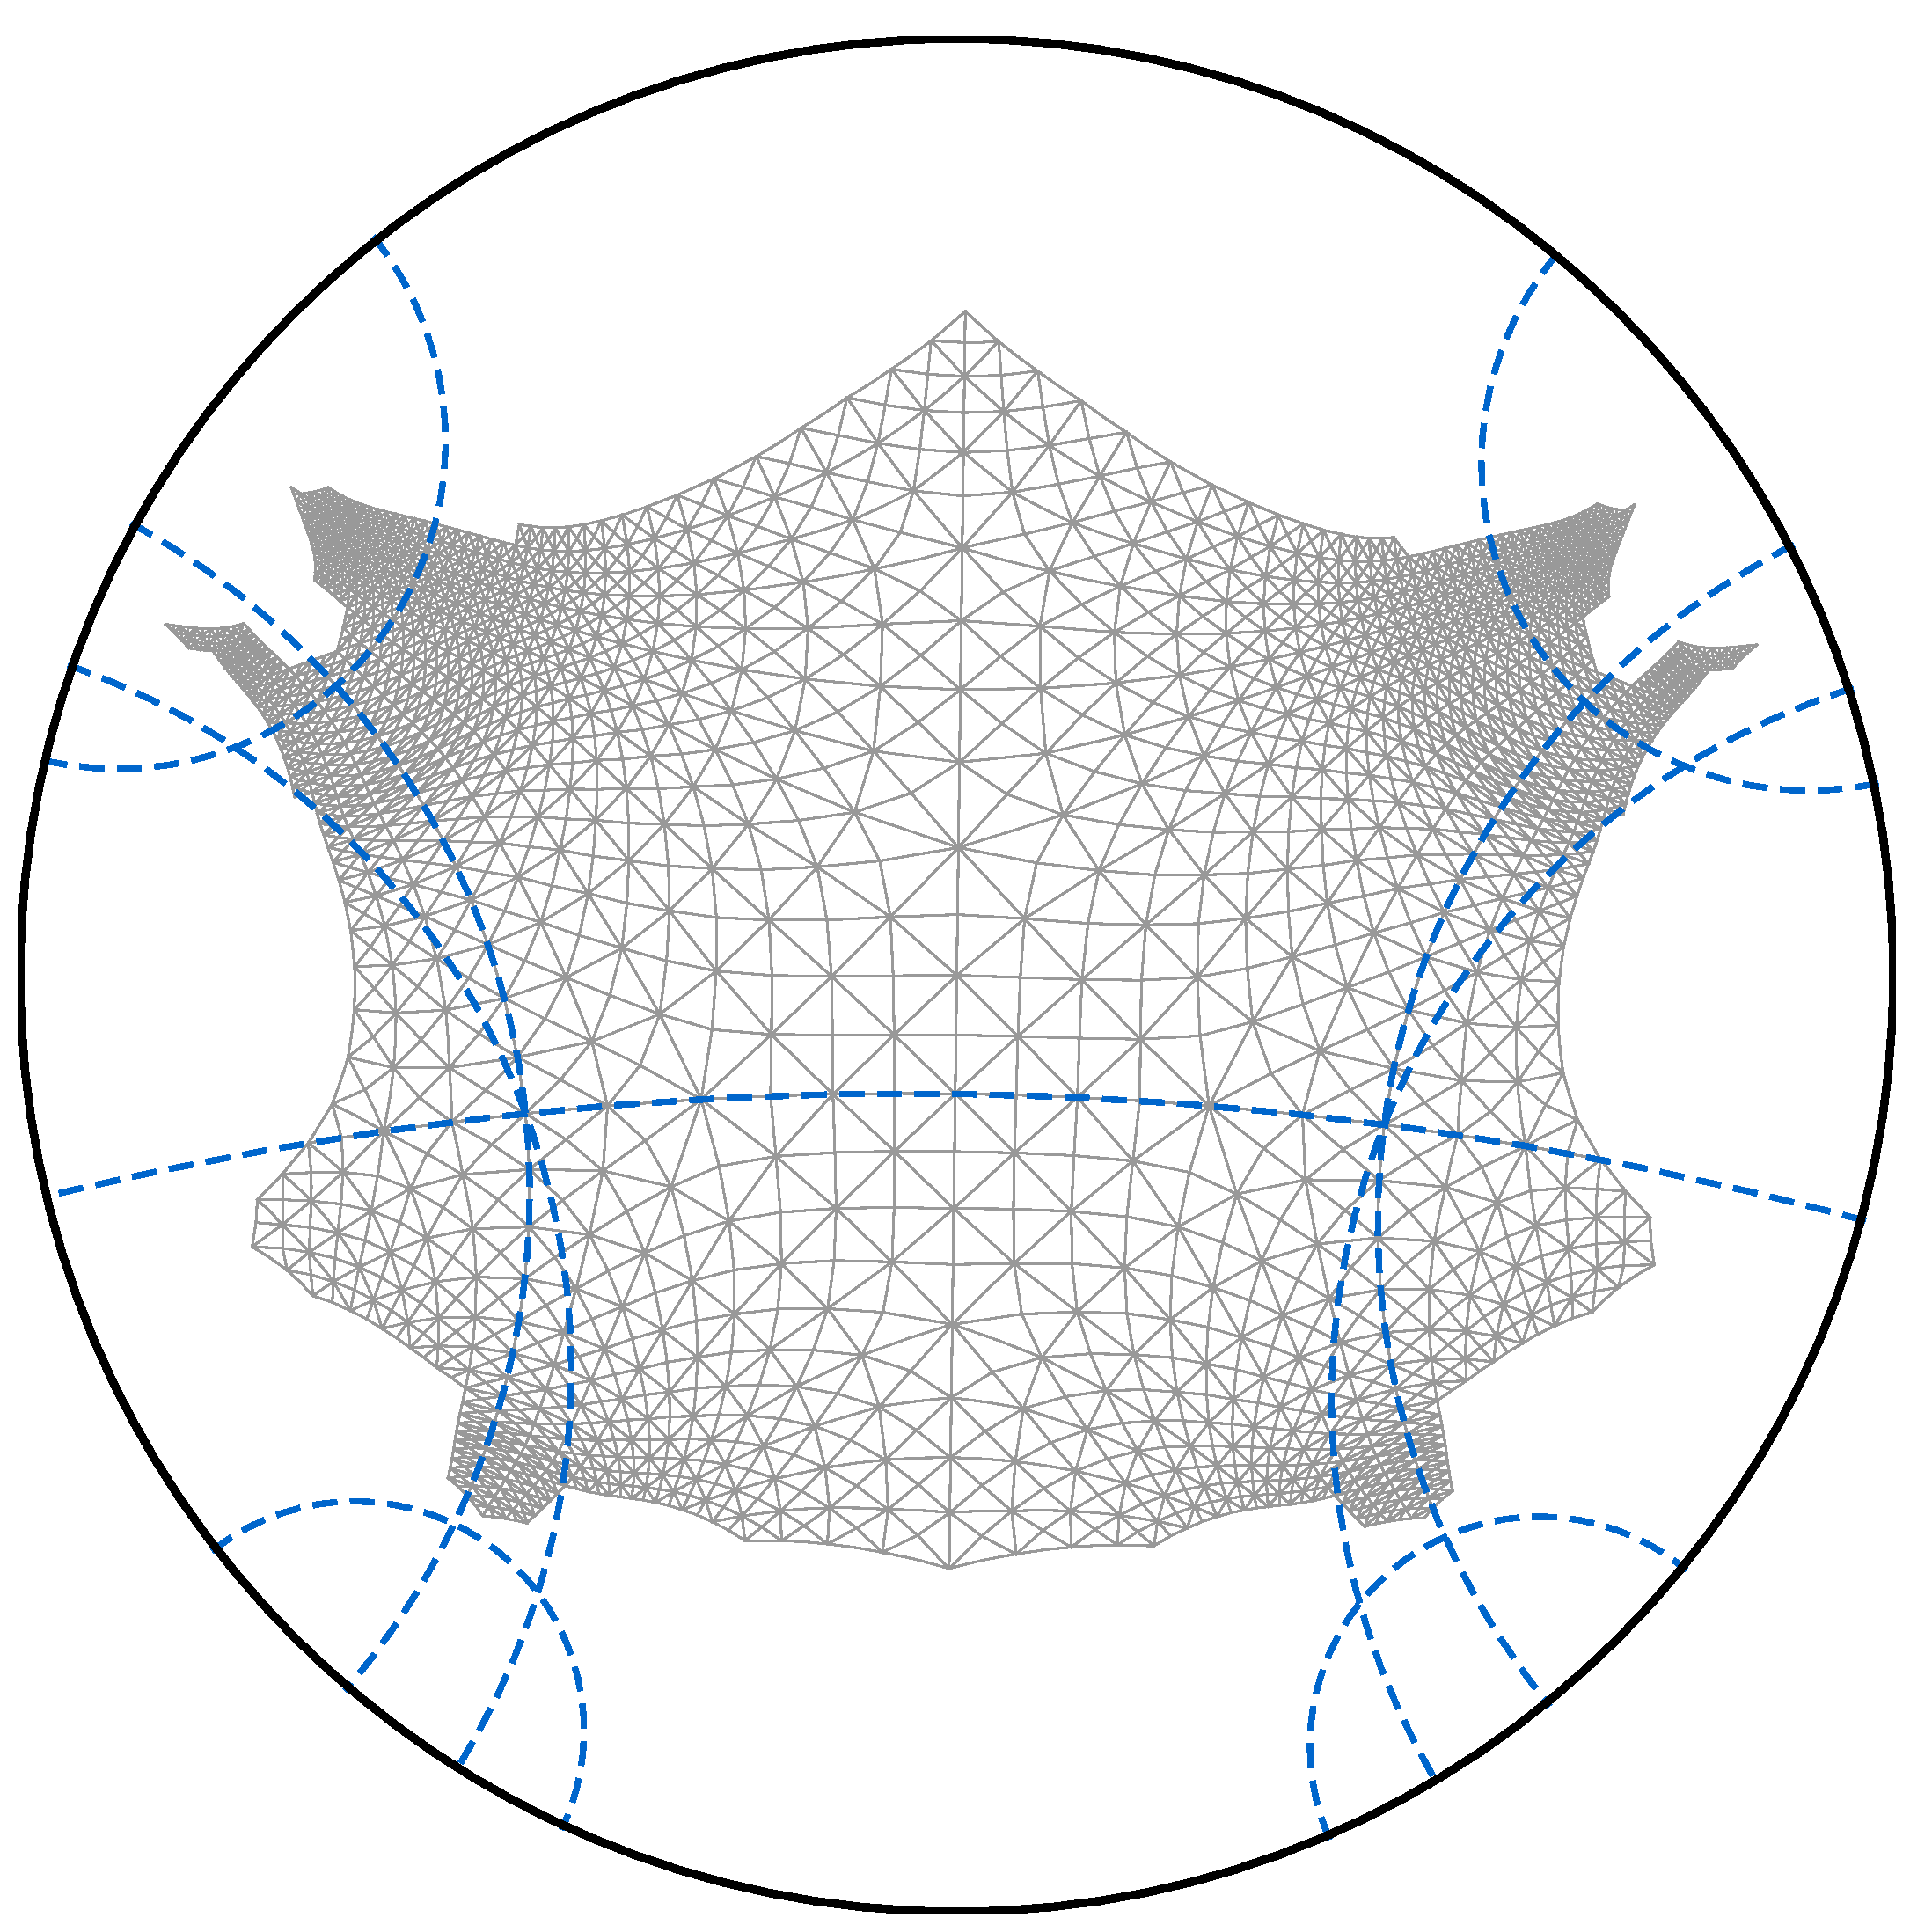
\includegraphics[width=0.4\linewidth]{cutCuttedBrezel01}
\caption{Hyperbolic flat metric on a genus $2$ surface and the axes of the associated hyperbolic motions.}
\label{fig:axes_of_motion}
\end{figure}

\subsection{Minimal presentation}
\subsection{Separated handles}
\subsection{Opposite sides identified}
\subsection{Canonical Keen Polygons}

\section{Uniformization of embedded genus $g=0$, $g=1$, and $g>1$ surfaces}

\section{Branched coverings of $\Chat$}
In this section we discuss surfaces that arise as branched coverings of $\hat{\C}$. A Riemann surface that can be represented as a double cover of $\Chat$ is called elliptic for $g=1$ and hyperelliptic for $g>1$~\cite[p.~235]{Jost2007}. 

Let $\lambda_1,\ldots,\lambda_{2g+2}\in \hat{\C}$, $\lambda_i\neq \lambda_j \forall i\neq j.$. The algebraic curve

\begin{equation}
\label{eq:branched_cover}
C=\{(z,w)\in\C^2 \mid w^2 = \prod_{i=1}^{2g+2}(z-\lambda_i)\}
\end{equation}

is a one dimensional complex manifold. A branched double cover of $\Chat$ is the projection $\pi:C\to\C$, $C\ni(z,w)\mapsto z$. A discrete branched cover of $\Chat$ is a triangulation of $\pi(C)$ with vertices at $\lambda_i$.

\subsection{Elliptic curves}
\subsection{The moduli space}
\subsection{Numerical convergence analysis}
\subsection{The modulus of the Wente torus}

\subsection{Construction of hyperelliptic surfaces}
Any hyperelliptic Riemann surface can be expressed as an algebraic curve of the form
\[ w^2 = \prod_{i=1}^{2g+2}(z-\lambda_i) \quad\quad g\geq1,\quad \lambda_i\neq \lambda_j \forall i\neq j.\]
Here $\lambda_i$ are the branch points of the doubly covered Riemann sphere.

\subsection{Weierstrass points on hyperelliptic surfaces}
A hyperelliptic surface comes together with a holomorphic involution $h$ called the hyperelliptic involution. The branch points are fixed points under this transformation. For a hyperelliptic algebraic curve it is $h(\mu, \lambda)=(-\mu, \lambda)$

\subsection{Canonical domains}
\subsection{Lawsons surface}

\section{Uniformization of Schottky data}
\subsection{Images of isometric circles}
\subsection{Hyperelliptic data}

\section{Conformal maps to $\Chat$}
\subsection{Selection of Branch Data}
\subsection{Examples}

\section{Surfaces with boundary}
\label{sec:surfaces_with_boundary}
\subsection{Variation of edge length}
\subsection{Examples}
\begin{figure}
	\centering
	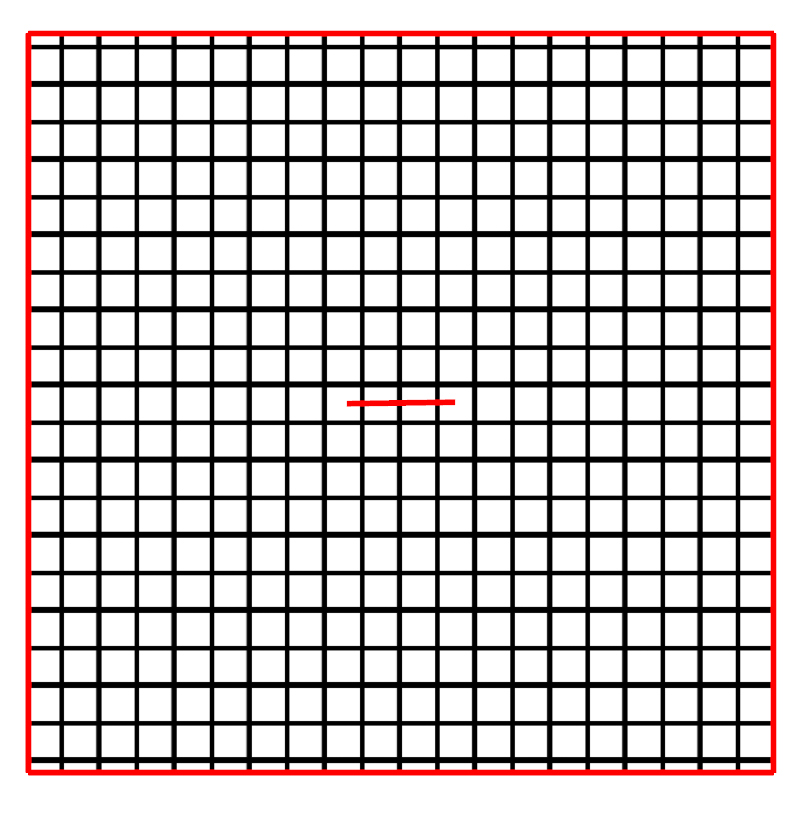
\includegraphics[width=0.3\linewidth]{image/slit_domain/domain_grid.png}
	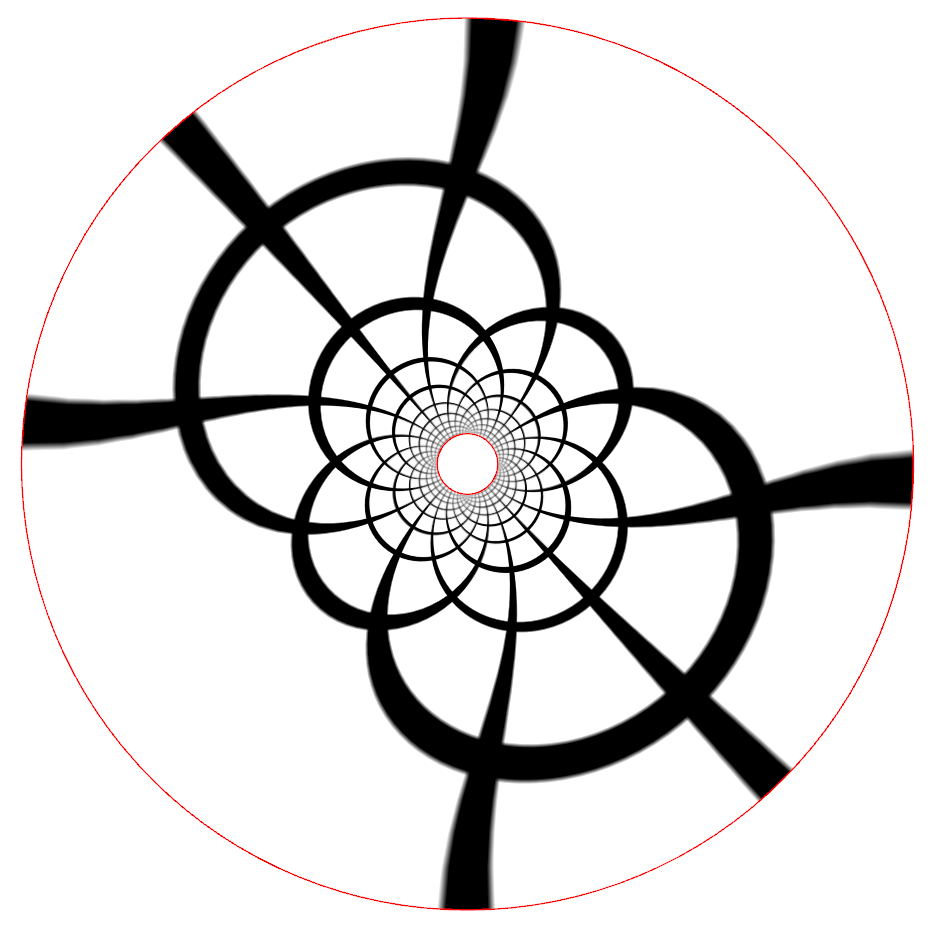
\includegraphics[width=0.3\linewidth]{image/slit_domain/image_grid.png}
	\caption{Square with symmetric slit to the circle}
	\label{fig:slit_circle}
\end{figure}


\section{Conformal maps of planar domains}
\label{sec:planar_domains}
\subsection{Boundary conditions}
\subsection{Comparison with examples of the Schwarz-Christoffel community}

%%% Local Variables:
%%% TeX-master: "Thesis.tex"
%%% End:
%\documentclass[Thesis.tex]{subfiles}
\begin{document}

\chapter{Quasiisothermic mesh layout}
\label{chp:quasiisothermic}

This chapter is joint work with Thilo R{\"o}rig and Alexander Bobenko.
Most of the material presented here was published previously in the proceedings of the conference "Advances in Architectural Geometry 2012"~\cite{Sechelmann2012}. We added Section~\ref{sub:isometric} on isometric deformations of s-isothermic surfaces and Section~\ref{sec:discrete_ellipsoid} about a discrete ellipsoid.

\emph{Abstract:} 
In architecture the quality of a quad-mesh depends on the shape of the individual
quadrilaterals. The ideal shape from an architectural point of view is the
planar square or rectangles with fixed aspect ratio. A parameterization that divides a
surface into such shapes is called isothermic, i.e., angle-preserving and
curvature-aligned. Such a parameterization exists only for the special class of
isothermic surfaces. We extend this notion and introduce quasiisothermic
parameterizations for arbitrary triangulated  surfaces.

We describe an algorithm that creates quasiisothermic meshes.
Interestingly many surfaces appearing in architecture are close to
isothermic surfaces, namely those coming from form finding methods and physical
simulation. For those surfaces our method works particularly well and gives a
high quality and robust mesh layout. We show how to optimize such meshes
further to obtain disk packing representations. The quadrilaterals of these
meshes are planar and possess touching incircles.

\begin{figure}
\centering
\resizebox{\textwidth}{!}{
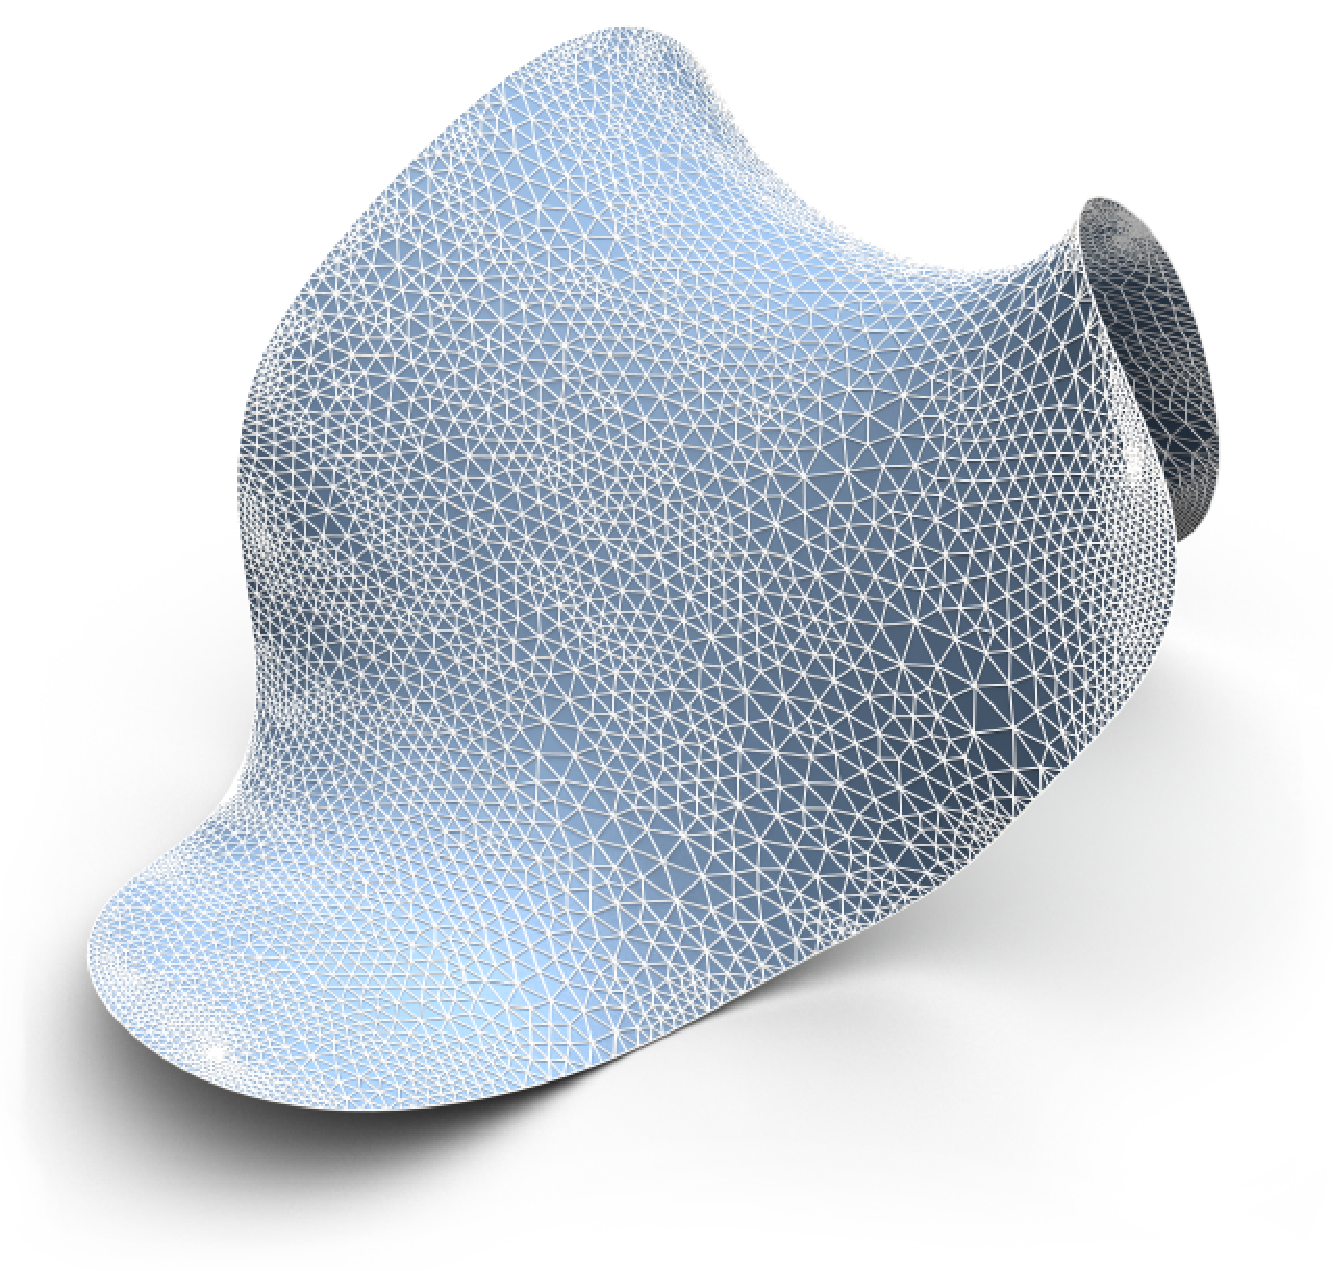
\includegraphics[width=0.48\linewidth]{image/aag2012/cover01.pdf}
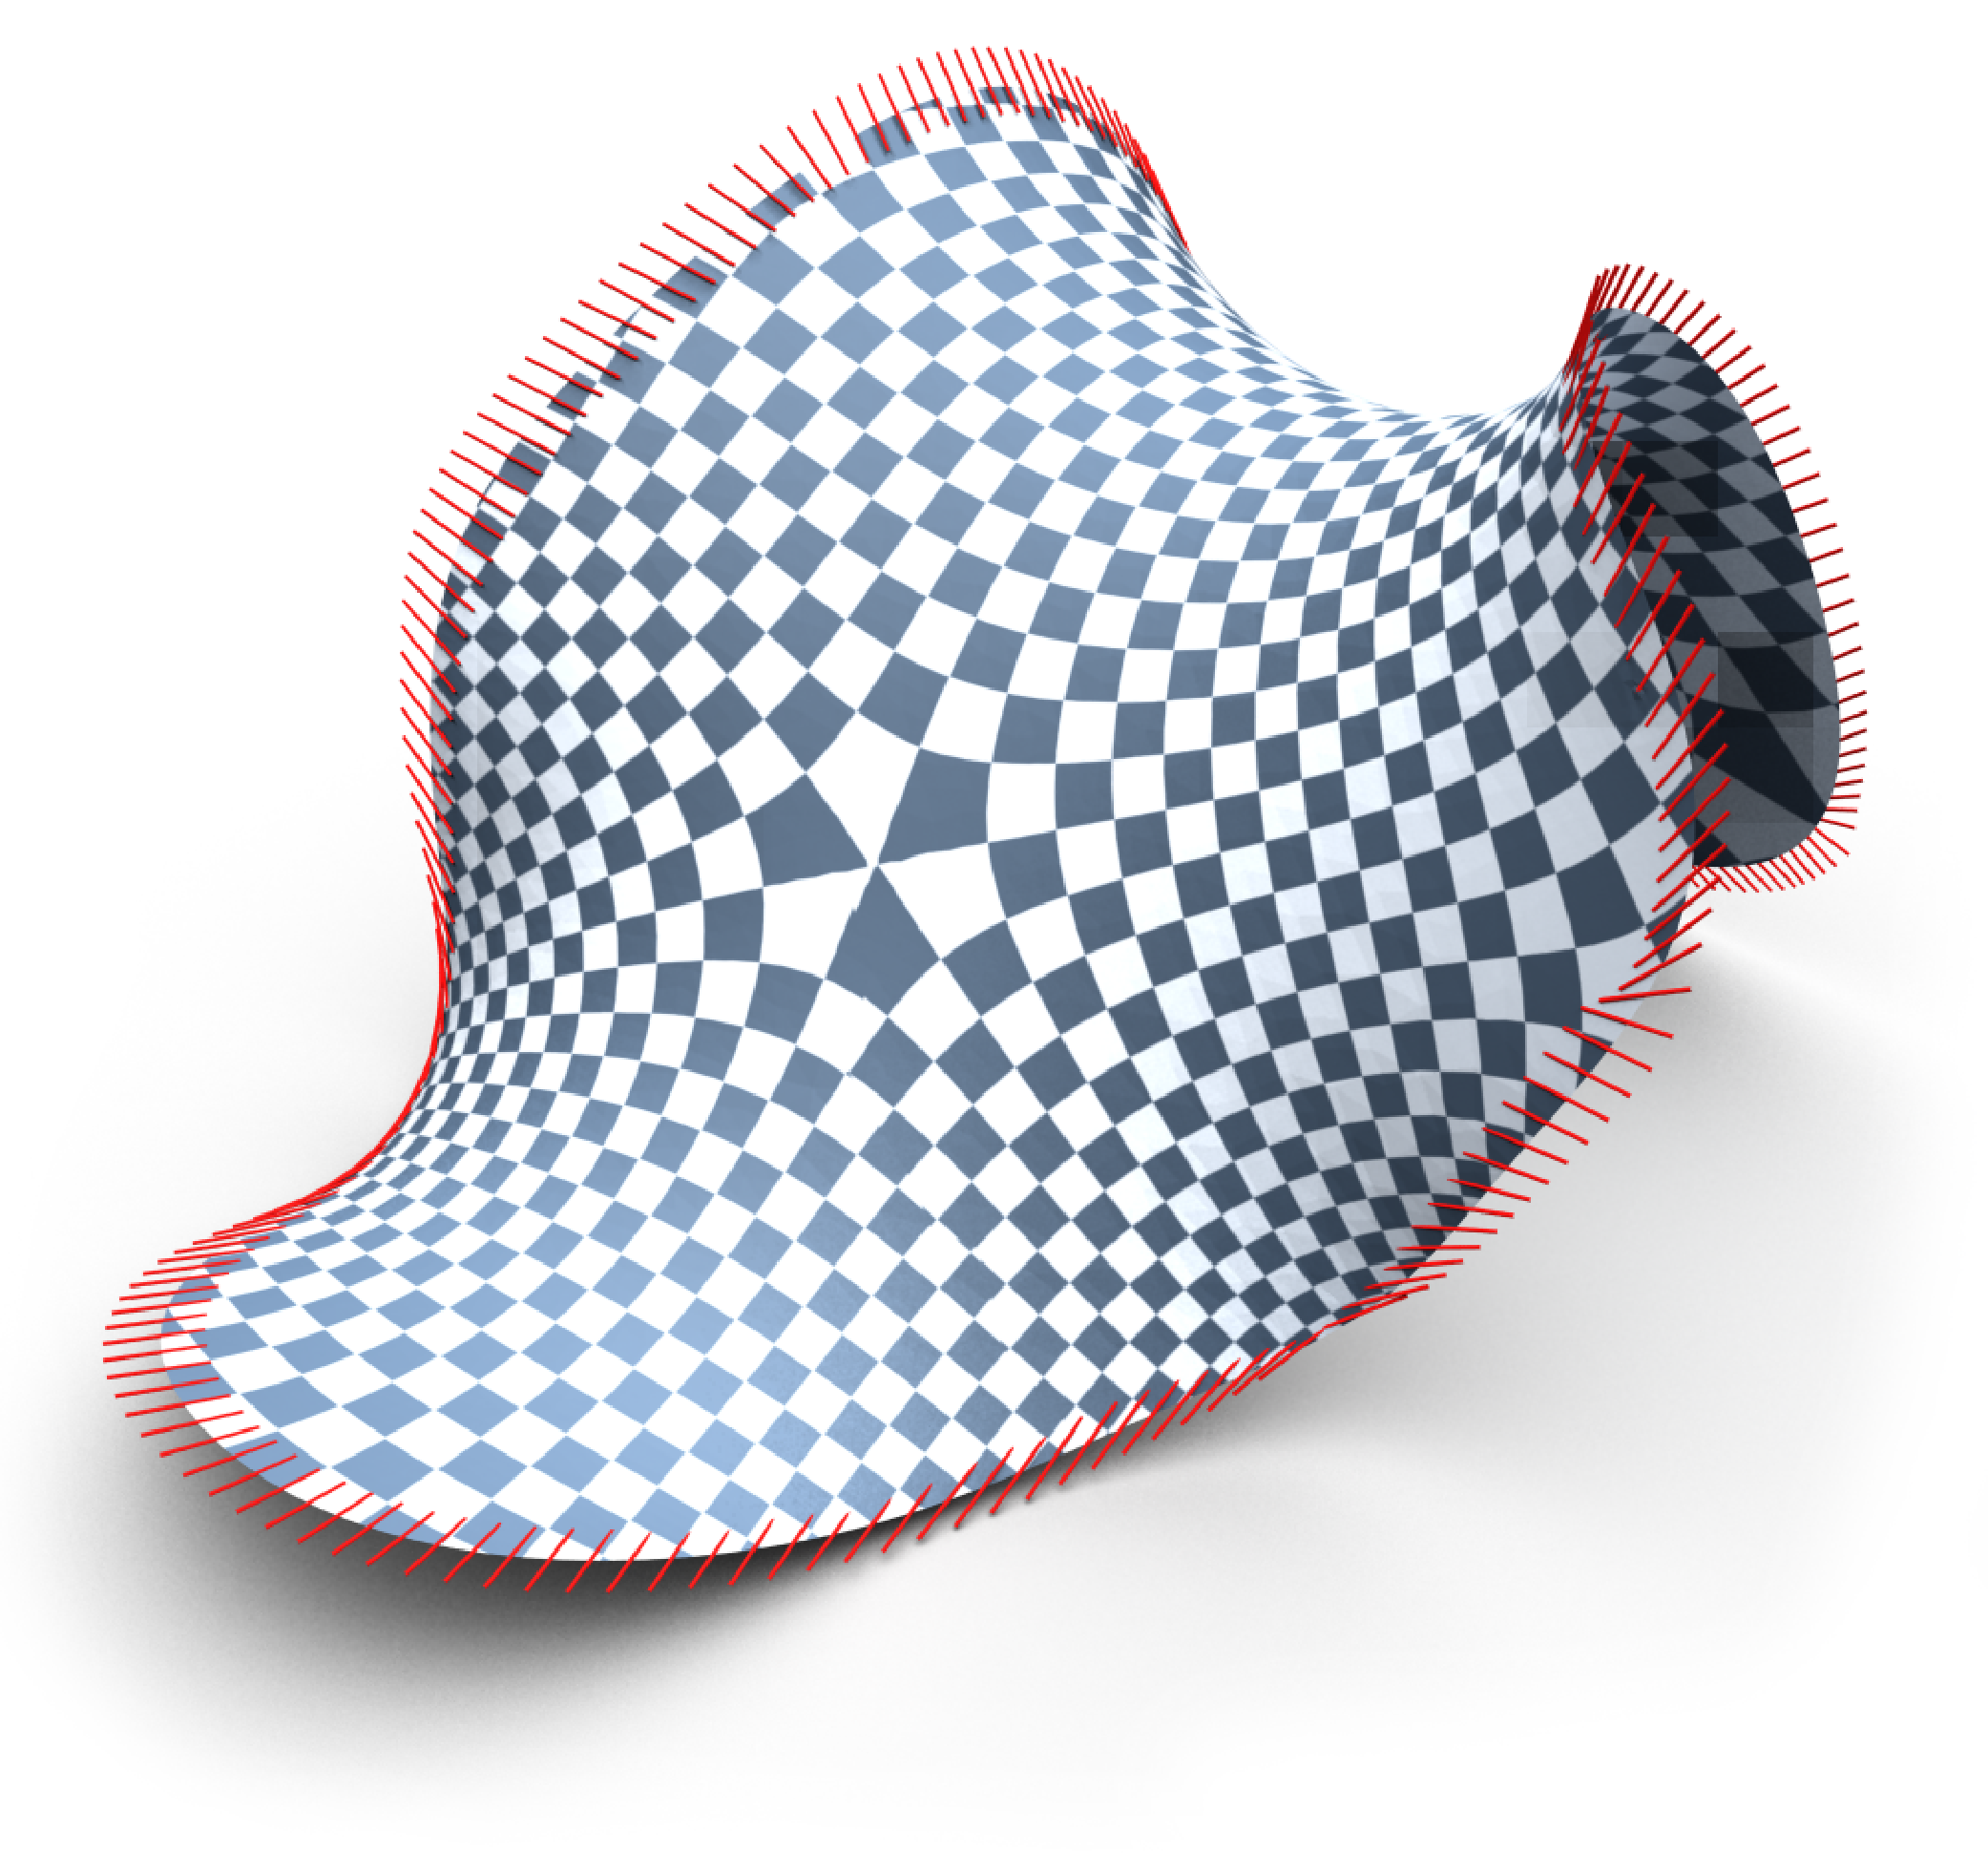
\includegraphics[width=0.48\linewidth]{image/aag2012/cover02.pdf}
}\\
\resizebox{\textwidth}{!}{
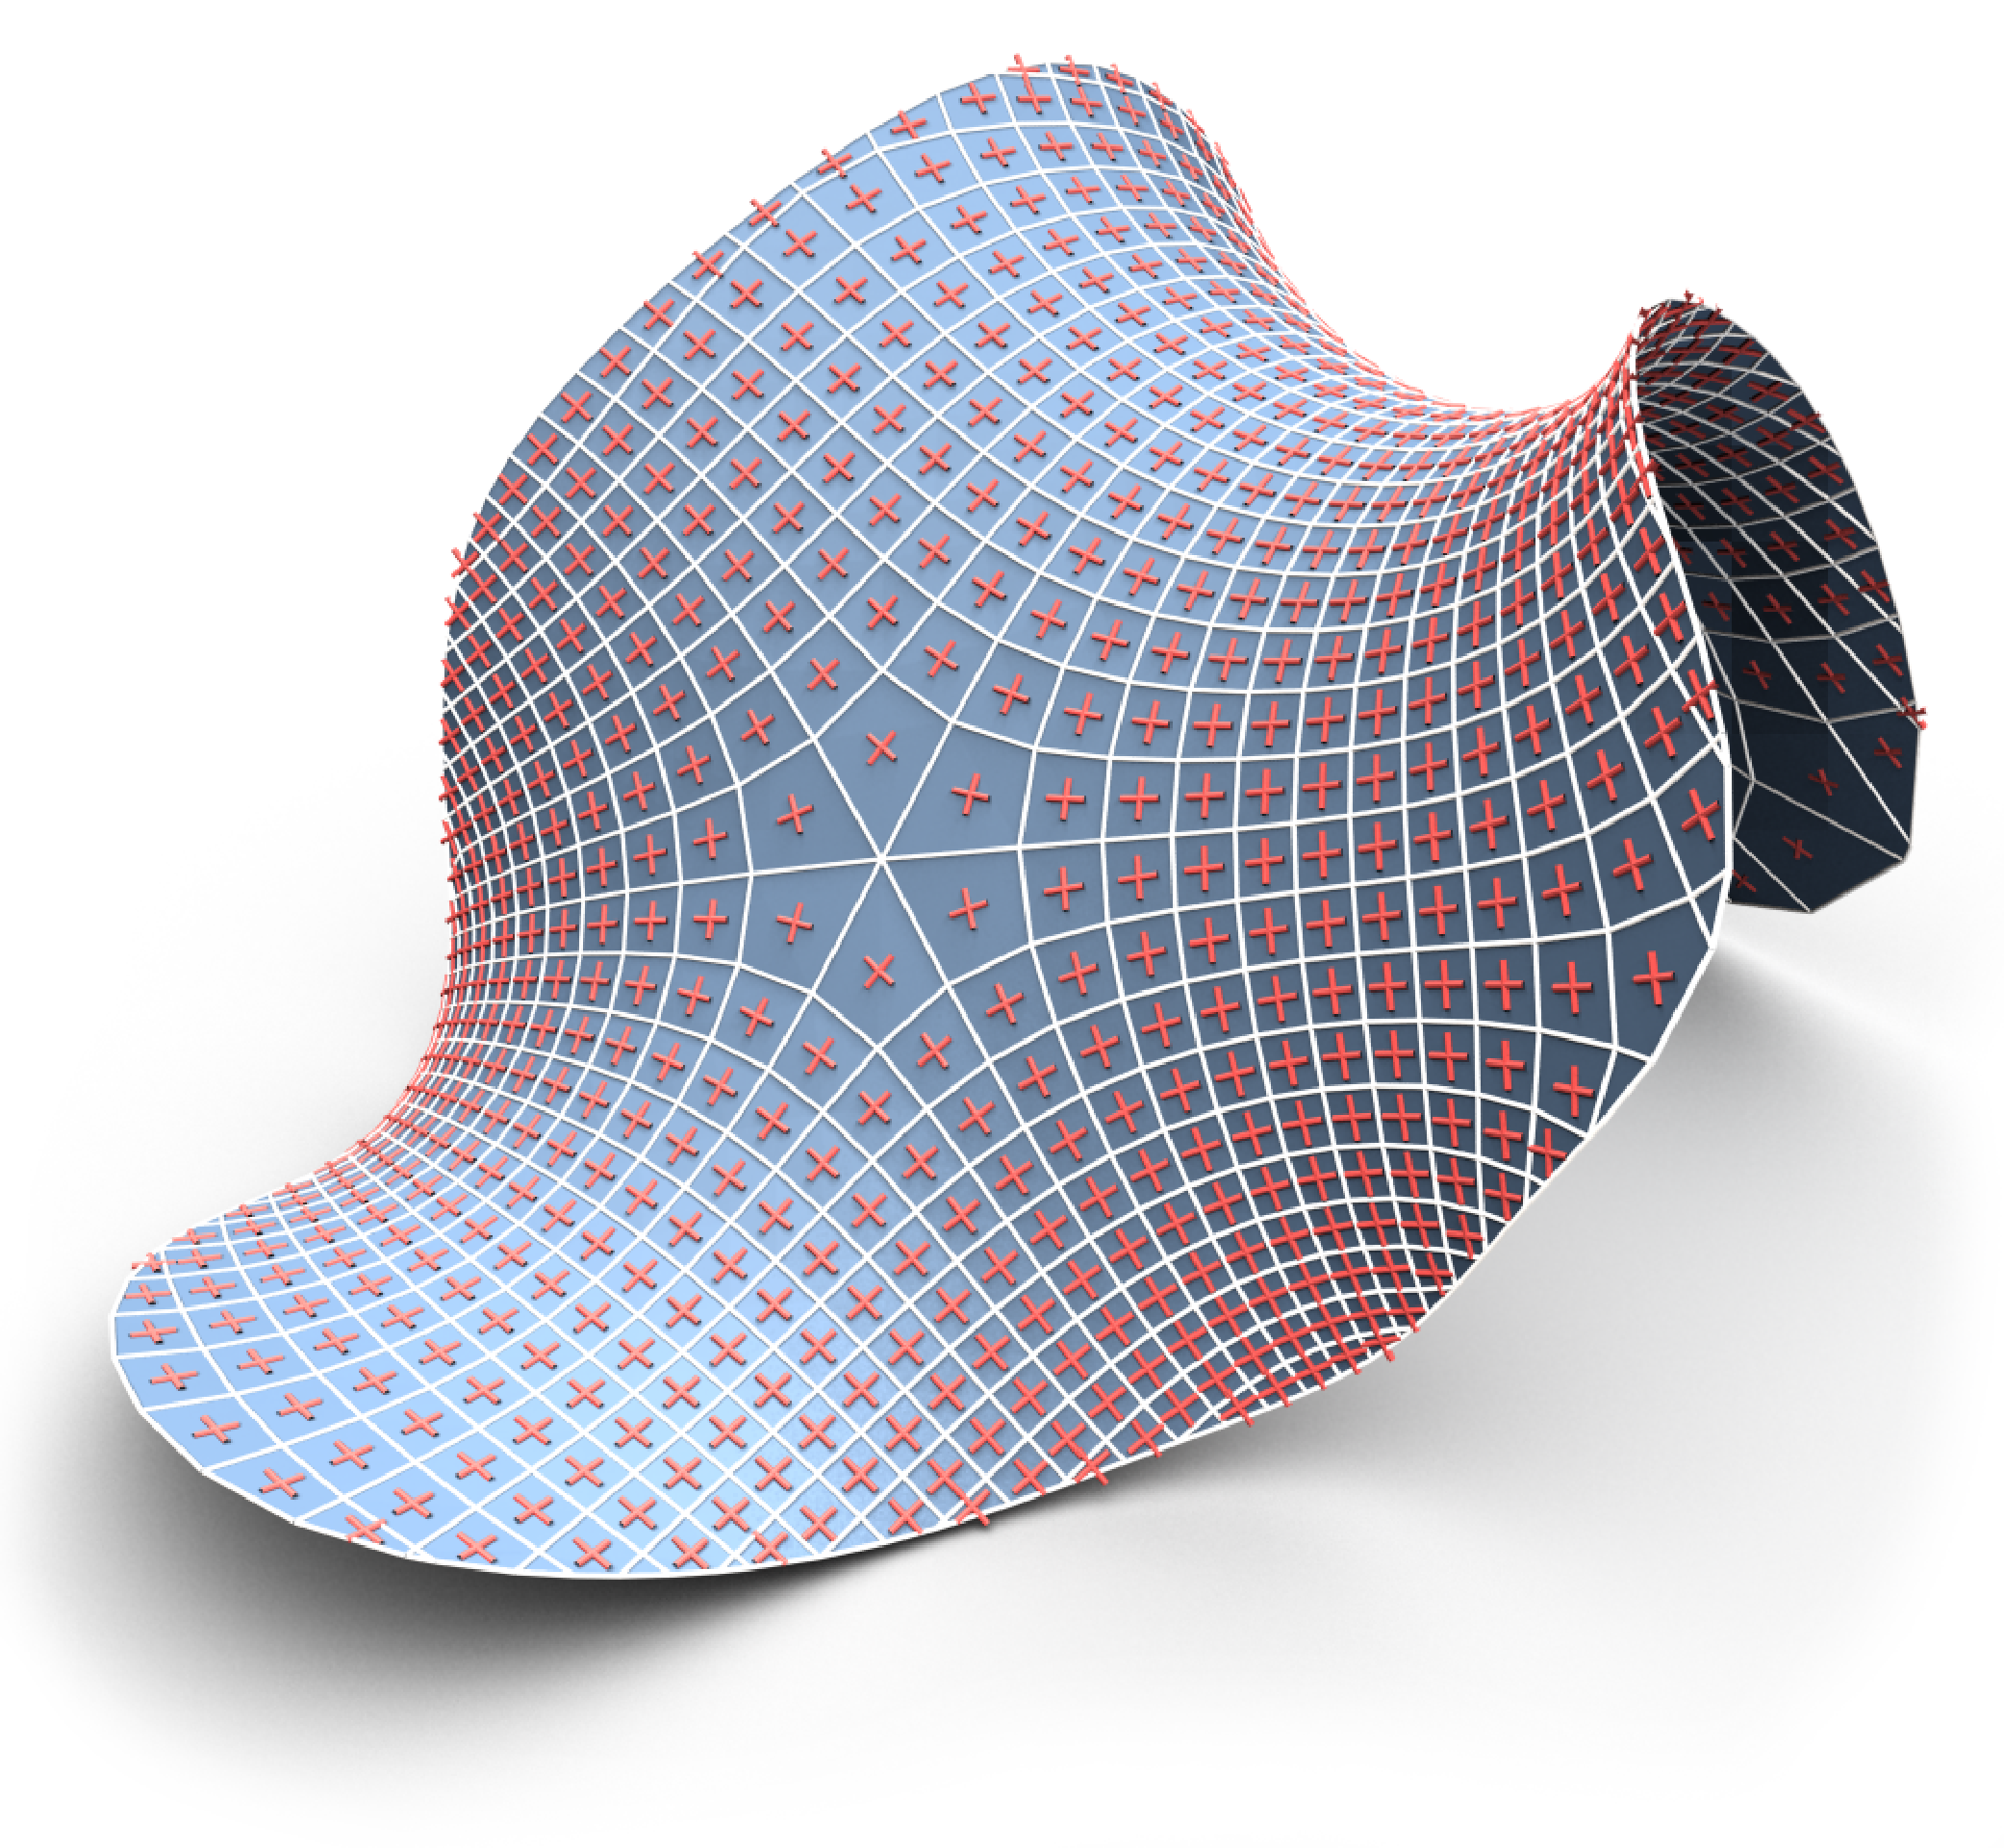
\includegraphics[width=0.48\linewidth]{image/aag2012/cover03.pdf}
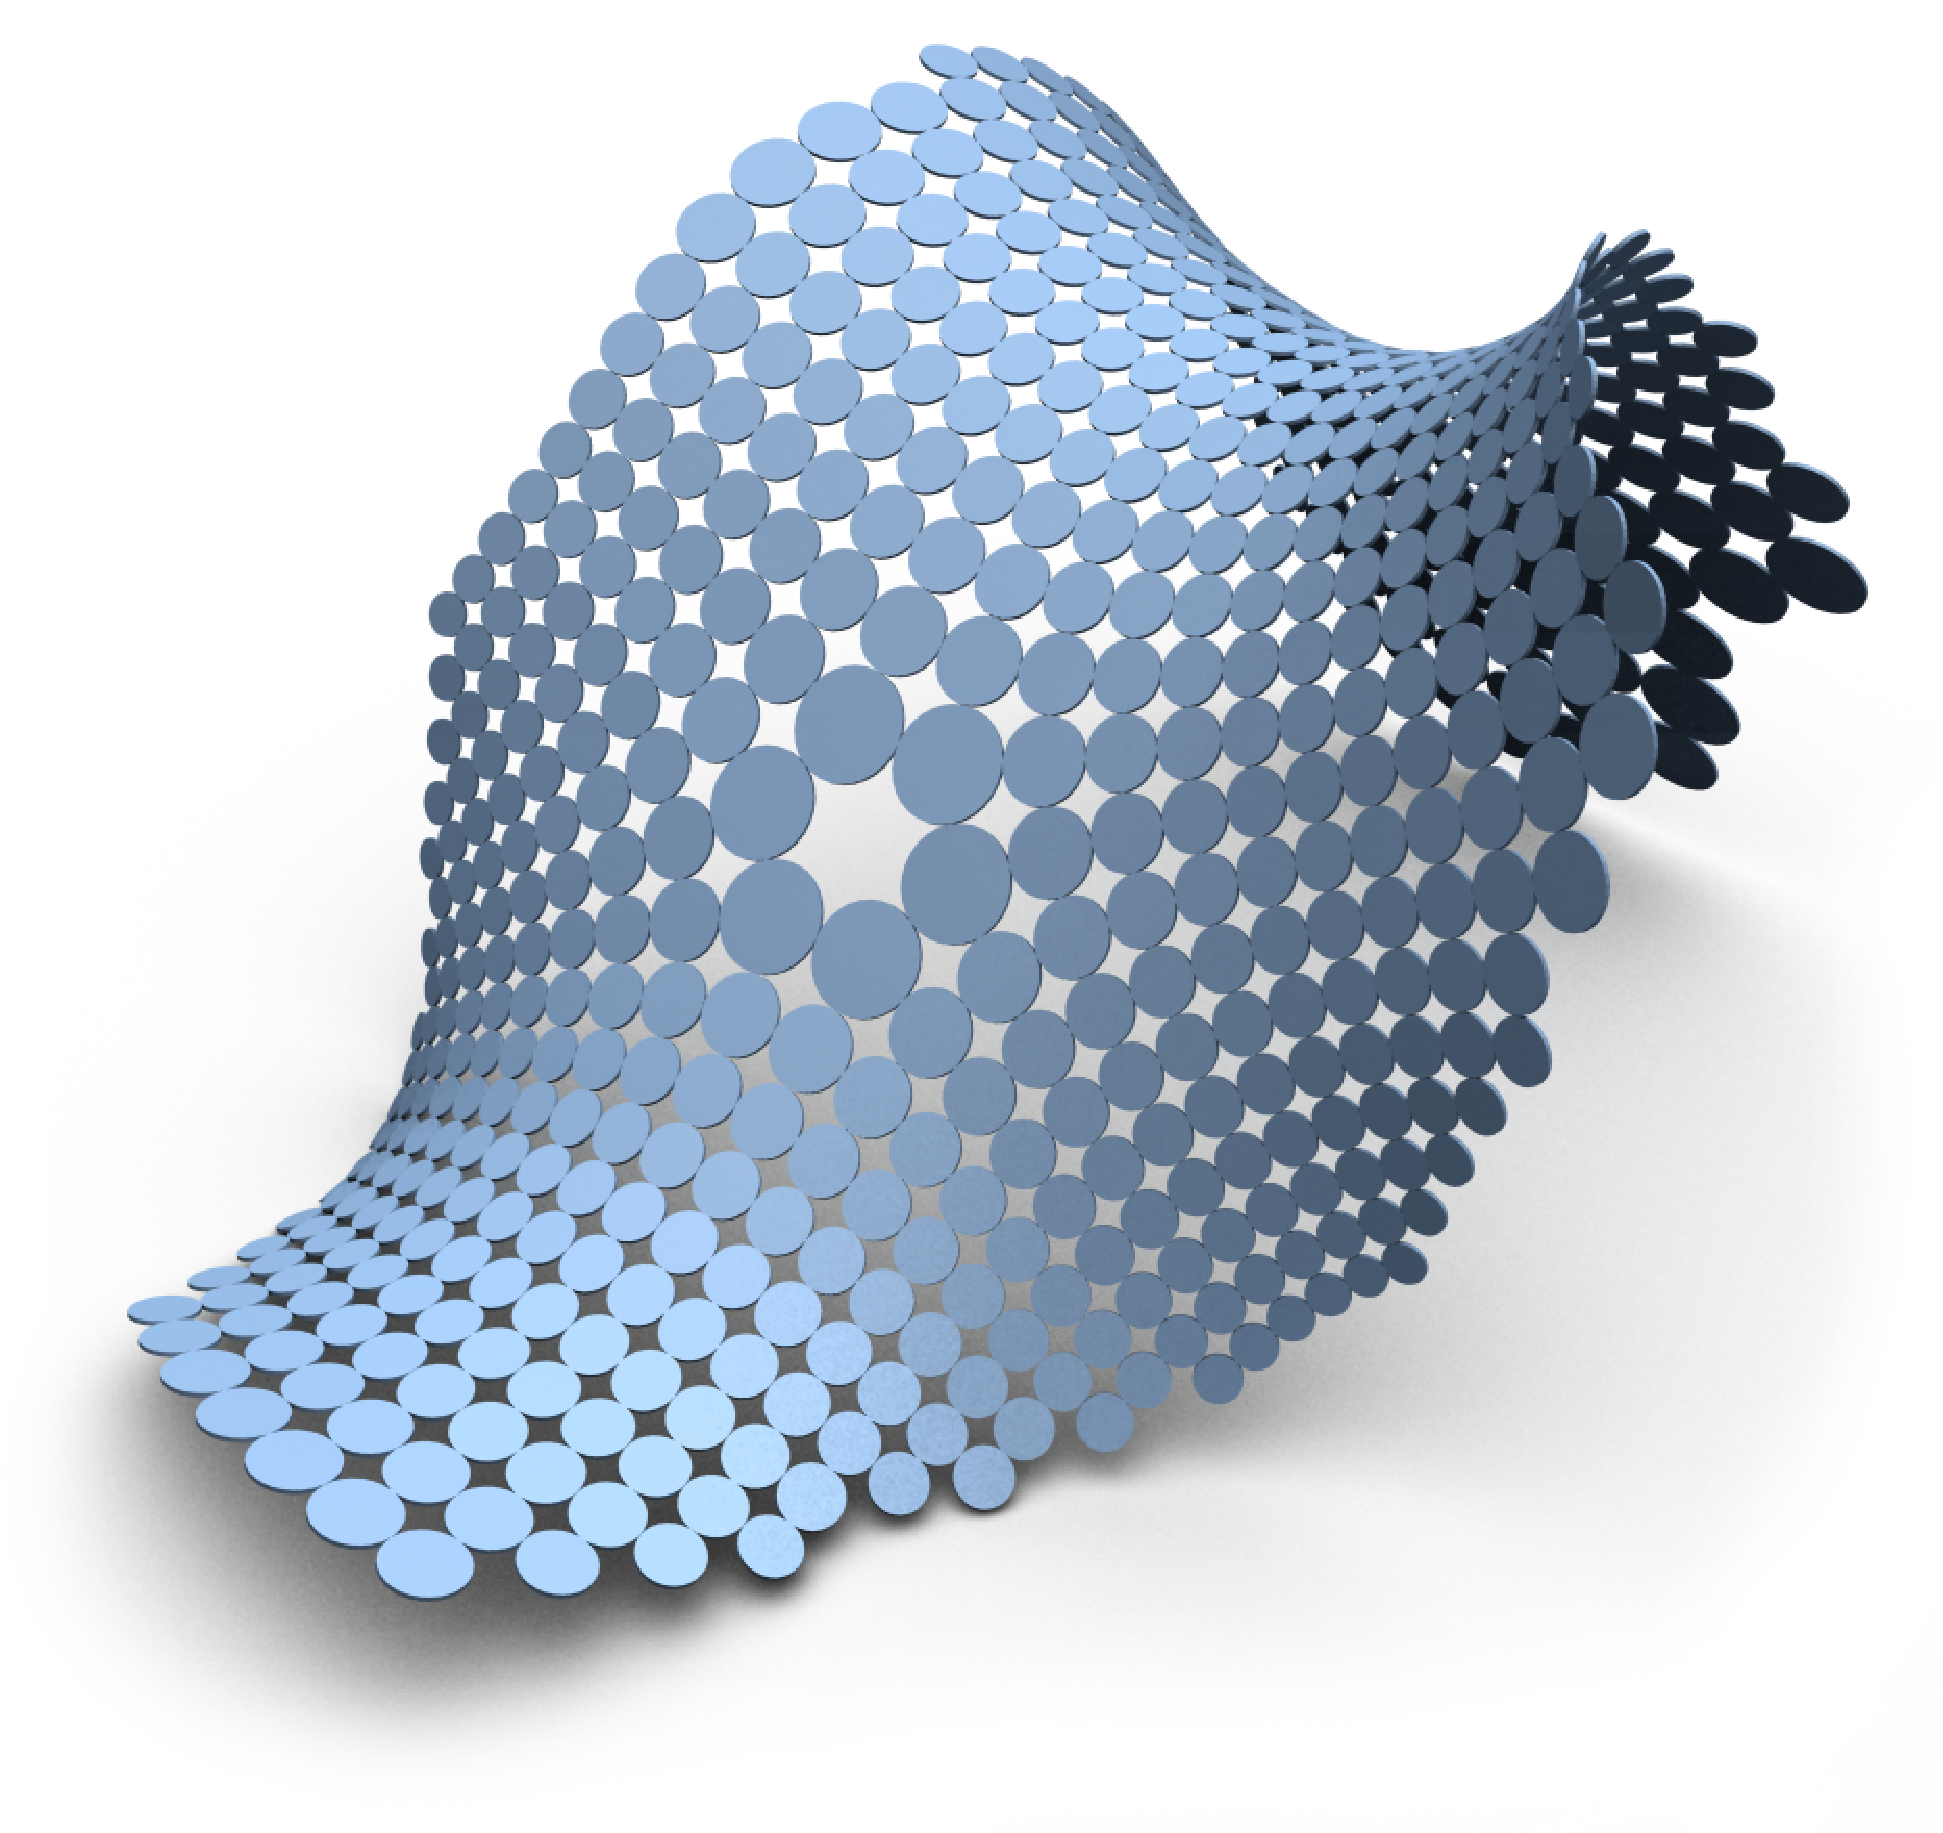
\includegraphics[width=0.48\linewidth]{image/aag2012/cover04.pdf}
}
\caption[Quasiisothermic parameterization step-by-step]{The algorithmic 
steps of this paper: For a triangulated surface we calculate 
texture coordinates by solving a boundary value problem for
principle curvature directions on boundary edges (checker board texture
and red directions). The edges of the corresponding quad mesh
align with the curvature directions (red crosses). The mesh is then
optimized towards planar quads with touching incircles.
}
\label{fig:teaser}
\end{figure}


\begin{figure}
\centering
\resizebox{\linewidth}{!}{\input{figures/all_mesh.pdf_t}}
\caption[Quasiisothermic parameterization: Examples]{The surface examples of this paper. All have been parameterized and
remeshed. $(a)$ The \textsc{Teaser} surface is the minimizer of a spring energy
with a smooth fixed boundary curve. $(b)$ A \textsc{Minimal} surface with
polygonal boundary curve. $(c)$ \textsc{Dome}: Part of a NURBS surface
exhibiting positive curvature and two curvature field singularities. $(d)$
\textsc{Roof} structure with planar boundary curve and regions of positive and
negative curvature.} 
\label{fig:all_mesh}
\end{figure}

\section{Introduction}
A key problem in architectural geometry is to convert surfaces created by form
finding methods, physical simulation, or manual modeling to quadrilateral
meshes, which are preferred for glass-steel structures. There are many 
possible quad-meshes that approximate a given shape and we study those that consist
of principle-curvature-aligned conformal squares, see Figure~\ref{fig:all_mesh}. 
Not all surface shapes can be approximated by such meshes. A smooth analog of
a surface with this property is called an isothermic surface. These surfaces admit conformal
curvature line parameterizations, i.e., angle-preserving parameterizations
aligned with the principle curvature directions. Their discrete counterpart are 
so-called s-isothermic meshes. These meshes have the additional property that
neighboring quadrilaterals possess touching incircles, see
Figure~\ref{fig:s_isothermic}.

The class of isothermic surfaces comprises, for example, constant mean
curvature surfaces. Roofs that act shell-like turn out to have almost constant
mean curvature. These are the kinds of surfaces that initiated our study of
conformal curvature line parameterizations in the architectural context. Both
conformality and alignment with curvature lines are favorable
properties for meshes. 

\noindent The contributions of this paper are:\\
\noindent\textbf{Definition of quasiisothermic parameterizations:} 
We propose a definition of quasiisothermic parameterizations of triangle meshes. 
It is based on angles between curvature directions and edges of a triangle mesh.
We define the quasiisothermic modulus that measures how isothermic a 
parameterization is. If this modulus is zero we obtain discrete isothermic 
parameterizations in the sense of our definition.

\noindent\textbf{Parameterization Algorithm:}
We give an algorithm that creates quasiisothermic parameterizations based on discrete
conformal maps of triangle meshes to the plane. This approach is built on top 
of the conformal mapping technique of Springborn~{\it et al.}~\cite{Springborn2008}. We
inherit the speed and superior projective mapping properties of their 
parameterizations.

\noindent\textbf{Variational principle for circle packing quad-meshes:}
The obtained parameterizations are used for remeshing and we optimize 
quadrilaterals to have touching incircles by minimizing a novel energy. These
s-isothermic meshes have been studied in discrete differential geometry and
possess some remarkable properties, e.g.,\ minimal s-isothermic surfaces may be
deformed isometrically retaining the same Gau{\ss} map.

The rest of the paper is organized as follows: Section~\ref{sec:previouswork}
gives an overview of existing parameterization schemes and their relation to
our approach. We also give reference to the related mathematical literature in
discrete differential geometry. In Section~\ref{sec:parametrization} we define
quasiisothermic parameterizations and a corresponding quality measure. 
In Section~\ref{sec:algorithm} we describe an algorithm to
obtain quasiisothermic parameterizations with small modulus. We describe the 
connection to discrete conformal maps and discuss how we deal with singularities. %XXX
A variational principle to generate s-isothermic meshes is presented in
Section~\ref{sec:s-isothermic}. At the end of the section we show the effect of
our optimization on several examples from different classes of surfaces. In the
final Section~\ref{sec:future} we sum up the results and propose extensions and
enhancements subject to further research.


\section{Related work}
\label{sec:previouswork}

There has been considerable work on conformal parameterizations as well as on
curvature line parameterizations related to our quasiisothermic scheme. We can 
only give a selection of previous work here.
% general parameterization 
For a general background on mesh parameterization we refer to the surveys by
Floater and Hormann~\cite{Floater2005} and Sheffer~\emph{et~al.}~\cite{ShefferPR2006}.

% conformal 
Our algorithmic approach is based on the discrete conformal equivalence of
triangle meshes as introduced by Springborn~\emph{et~al.}~\cite{Springborn2008} (see the work of
Bobenko~\emph{et~al.}\ for the mathematical background~\cite{BPS2015:dconf}). The
convex functional optimized by Springborn~\emph{et~al.}\ constructs a conformally
equivalent flat mesh for specified boundary conditions and singularities. 
Our method is related to work on angle based flattening by Sheffer and de~Sturler~\cite{Sheffer2001}. They aim for conformal parameterizations 
and express this by the additional constraint, that triangle angles have to be close 
to the original ones on the surface. For discrete isothermic parameterizations 
the definitions coincide.
%A different approach based on circle patterns is used by
%\cite{KharevychSSCircle06} to produce conformal mappings from a surface to the
%plane. Global conformal parameterizations for surfaces of arbitrary topology
%were constructed by \cite{GuYauConformal03}.

% curvature line 
Parameterizations aligning with lines of principle curvature were constructed
by Alliez~\emph{et~al.}~\cite{AlliezCDLD2003}. Their method involves 
the integration of curvature vector fields
and does not include an optimization towards conformality. 
Global parameterizations following arbitrary frame fields 
(including in particular principle curvature fields) are constructed
in the work of K\"{a}lberer~\emph{et~al.}~\cite{KalbererNP2007}. They use 
discrete Hodge decomposition and
harmonic vector fields to obtain a globally consistent parameterization. Their
QuadCover algorithm can deal with surfaces of arbitrary genus and treats
singularities using a suitable branched cover.
Both algorithms cover arbitrary triangulated surfaces and implementations are
highly complex.

% circles on surfaces 
The use of variational principles to enforce desired properties such as planarity of 
quadrilateral faces has been successfully used in architectural geometry.
Liu~\emph{et~al.}~\cite{LiuPWYW2006} propose an algorithm to optimize a quadrilateral mesh to
become planar and even conical. Pottmann~\emph{et~al.}~\cite{PottmannSBSWBW2008} use functionals to
approximate freeform surfaces with single curved panels. The energy minimized in
Section~\ref{sec:s-isothermic} is a combination of a new functional with an
energy recently described by Schiftner~\emph{et~al.}~\cite{SchiftnerHWP2009}. They construct circle
packing triangle meshes that approximate a given surface by minimizing a
combination of energies. 

Discrete s-isothermic minimal surfaces are defined in
terms of their Gau{\ss} map by Bobenko~\emph{et~al.}~\cite{BobHofSpr06}. 
This Gau{\ss} map is a Koebe
polyhedron with edges tangent to a sphere. These Koebe polyhedra also occur in
the study of edge offset meshes by Pottmann~\emph{et~al.}~\cite{PottmannLWB2007}, 
who again use a
variational approach to obtain support structures. Another parametrization
technique creating quad-dominant meshes guided by conjugate parameter
directions is given by Zadravec~\emph{et~al.}~\cite{ZadravecSW2010}. Their algorithm 
includes a level
set approach to circumvent the integration of a vector field.

The notion of discrete s-isothermic meshes was introduced in the mathematical
context by Bobenko and Pinkall as a special class of quad meshes~\cite{BobenkoP1996}.
The mathematical theory of these meshes has since then been an active field of
research in discrete differential geometry. A good overview of the recent
development and literature can be found in the book by Bobenko and Suris~\cite{BobenkoSuris2008}. 


\section{Discrete quasiisothermic parameterization}
\label{sec:parametrization}
In this section we introduce the notion of quasiisothermic parameterizations and the
corresponding quality measure.

\subsubsection{Discrete parameterizations}
Let $M=(V,E,F)$ be a triangle mesh. The elements of $V$ are the vertices of the
mesh denoted by simple indices $i\in V$. Edges are denoted by double
indices $\mathrm{\it{ij}}\in E$, and faces are denoted $\mathrm{\it{ijk}}\in F$. A triangulated surface is
a map $S:V\to \mathbb R^3$, $i \mapsto (x_i, y_i, z_i)$.
We call a map $\Phi: V \to \mathbb R^2$, $i \mapsto (u_i,v_i)$ a \emph{discrete
parameterization} of the surface $S$. We only consider orientable surfaces and
parameterizations that preserve the orientation of the triangles with respect to
the canonical orientation of $\mathbb R^2$. 

The next definition connects arbitrary parameterizations with certain directions
tangent to the surface $S$, e.g., curvature directions. Such a direction is encoded as 
an angle per edge. 
%XXX: Ueberleitung; discrete $\alpha$-parameterization? 
% definition parameterization with \alpha
\begin{definition}
Let $\alpha : E \to ]-\frac{\pi}{2},\frac{\pi}{2}]$, $\mathrm{\it{ij}} \mapsto \alpha_{\mathrm{\it{ij}}}$
be a map that assigns an angle to each edge. A discrete parameterization 
$\Phi: V\to \mathbb R^2$, $i \mapsto (u_i,v_i)$ is called a \emph{discrete
parameterization with $\alpha$} if
\begin{equation}
\label{eq:isothermic}
\tan \alpha_{\mathrm{\it{ij}}} = \frac{u_i - u_j}{v_i - v_j}
\end{equation}
for all edges of the mesh.
\end{definition}
In other words, in a parameterization with $\alpha$ the image of an edge $\mathrm{\it{ij}}\in
E$ under the map $\Phi$ encloses the prescribed angle $\alpha_{\mathrm{\it{ij}}}$ with the
$v$-axis of the parameter space. One could equally use the $u$-axis here.

\begin{figure}
\centering
\resizebox{\textwidth}{!}{\input{figures/isothermic.pdf_t}}
\caption{A discrete isothermic parameterization. Angles between triangle edges 
and a curvature direction family are preserved by the map.}
\label{fig:isothermic_parameterization}
\end{figure}

\subsubsection{Quasiisothermic parameterizations}
Our main example of a parameterization with an angle function $\alpha$ comes
from $\alpha$ defined by the curvature directions of a surface $S:V\to
\mathbb R^3$ (see Fig.~\ref{fig:isothermic_parameterization}). For a triangulated surface 
curvature directions and magnitudes can be calculated and assigned to edges. This 
is usually done by averaging curvature information over neighborhoods of points 
on the surface \cite{CohMor03}. A discrete parameterization 
with angle function $\alpha$ stemming from the curvature direction field is then called a
\emph{discrete isothermic parameterization}. Indeed, the latter is just a
curvature line parameterization. In our case the curvature directions
are mapped to the coordinate directions in the $(u,v)$-plane. The map can be
treated as conformal: Angles between edges and curvature directions are 
preserved.

Generic surfaces do not allow for isothermic parameters (those admitting
isothermic parameterizations are called isothermic surfaces). Therefore we do
not expect a parameterization with given $\alpha$ to exist in general. To be
able to deal with arbitrary surfaces we introduce the notion of discrete
quasiisothermic parameterization. The idea is to obtain a parameterization with
angles $\tilde\alpha$ as close to the curvature directions $\alpha$ as possible.
Let
\begin{equation}
Q^\alpha(\mathrm{\it{ij}})=\left|\alpha(\mathrm{\it{ij}}) - \tilde\alpha(\mathrm{\it{ij}})\right|
\label{eq:quasiisothermicity}
\end{equation}
where $\tilde\alpha(\mathrm{\it{ij}})$ is angle the between the $v$-axis and the edge $\mathrm{\it{ij}}$ in 
parameter space.
\begin{definition}
We call a discrete parameterization $\Phi$ with angle function $\alpha$ 
\emph{quasiisothermic} with modulus $Q\in \mathbb R_+$ if
\begin{equation}
Q^\alpha(\mathrm{\it{ij}}) \leq Q
\end{equation}
for all edges $\mathrm{\it{ij}}\in E$.
\end{definition}
The motivation for this measure of quasiisothermicity is the following: If $Q$ is small
the directions of principle curvature on the surface are almost tangent to the parameter 
lines of the parameterization. For a modulus of zero we have an in a sense angle 
preserving map where edges enclose the same angles with the coordinate axes in 
parameter space as with curvature directions on the surface. We will now 
create parameterizations that have small $Q$.


\section{Minimization of the functional}
\label{sec:algorithm}

In this section the surface $M$ is a triangulated surface with one boundary
component. We will now construct a function $\Phi$ that
has zero approximation error $Q^\alpha$ at boundary edges and is a discrete
conformal map in the sense of Springborn~\emph{et~al.}~\cite{Springborn2008} in the 
interior of the
surface. We argue under which circumstances this leads to nice
behaviour in the interior. We start by briefly introducing discrete conformal
maps and the boundary conditions we need for our purposes.

\subsubsection{Discrete conformal maps}
\label{subsub:discrete_conformal_maps}

We recall the definition by Springborn~\emph{et al.} of discrete conformal 
maps via conformal equivalence of triangle meshes. It is stated in terms of
lengths of the surface edges and corresponding parameter edges in the 
$(u,v)$-plane.
\begin{definition} 
  A discrete parameterization~$\Phi$ is \emph{conformal} if there exists a
function $\mu:V \to \mathbb{R}$, $i \mapsto \mu_i$ such that the following
condition for the edge lengths $l_{\mathrm{\it{ij}}}$ on the surface and
$\tilde{l}_{\mathrm{\it{ij}}}=\Vert\Phi(i)-\Phi(j)\Vert$ in parameter space holds
\begin{eqnarray}
  \label{eq:discrete_conformal} 
  \tilde{l}_{\mathrm{\it{ij}}}=\mu_i\mu_j l_{\mathrm{\it{ij}}}.
\end{eqnarray}
\end{definition}
%XXX (u,v)-plane vs. function u
For a given triangle mesh there is a unique solution $\mu$ that retains the 
boundary edge lengths. Another unique solution can be obtained by fixing 
the angles between consecutive boundary edges. These angles have to be 
chosen consistently obeying the Gau\ss-Bonnet relation 
(see the section about singularities).

The function~$\mu$ for a given triangle mesh can be found as the minimizer 
of a convex functional. Thus its computation is efficient. The resulting 
parameterization is created by a breadth-first layout that enumerates 
all triangles and assigns texture coordinates. In addition to boundary angles 
one can ask for solutions that contain special interior vertices where the
 sum of triangle angles is not equal to $2\pi$ (see Fig.~\ref{fig:teaser}). 
These so-called cone points will be inserted at singularities of the 
parameterization.


\subsubsection{Curvature boundary conditions}
\label{subsub:boundary}

\begin{figure}
\centering 
\resizebox{\textwidth}{!}{\input{figures/boundary_conditions2_horizontal.pdf_t}}
\caption[Curvature boundary conditions]{Curvature boundary conditions: In parameter space the interior angle 
$\theta_j$ at the vertex~$\Phi(j)$ has to be chosen such that curvature 
directions given by angles $\alpha_{\mathrm{\it{ij}}}$ and $\alpha_{\mathrm{\it{jk}}}$ align with the 
$v$-axis. This choice is unique up to addition
of $k \pi$. The above pictures show two possible layouts in the parameter
plane depending on the interior angle sum on the surface.}
\label{fig:boundary_angles}
\end{figure}

Let $\alpha:E\to ]-\frac{\pi}{2},\frac{\pi}{2}]$ be an angle function derived
from numerical curvature directions and the given surface orientation. 
Let $\mathrm{\it{ij}}\in E$ and $jk\in E$ be two consecutive boundary edges with common
vertex $j$ and let $\tilde\theta_j$ be the sum of interior triangle angles on
the surface at this vertex.  The direction of the edge $\Phi(\mathrm{\it{ij}})$ (resp.\
$\Phi(\mathrm{\it{jk}})$) is determined by the angle $\alpha_{\mathrm{\it{ij}}}$ 
(resp. $\alpha_{\mathrm{\it{jk}}}$),
since the curvature directions encoded by the $\alpha$'s should align with the
$v$-axis. The orientation of the surface (resp.\ the boundary edges) defines
the angle $\theta_j$ between the edges $\Phi(\mathrm{\it{ij}})$ and $\Phi(\mathrm{\it{jk}})$ up to
addition of $k \pi$ (see Fig.~\ref{fig:boundary_angles}). To make the angle
unique we require that the difference between the original surface angle
$\tilde\theta_j$ and the angle in the parameter plane $\theta_j$ is as small
as possible, i.e.,\ choose $k>0$ as small as possible such that 
\[
|\underbrace{\angle(\Phi(\mathrm{\it{ij}}),\Phi(\mathrm{\it{jk}}))+ k \pi}_{\theta_j} - \tilde\theta_j| \le \pi/2.
\]
See Figure~\ref{fig:boundary_angles} for an
illustration of the alignment in the parameter plane. The angles $\theta_j$ at
boundary vertices serve as boundary conditions for the discrete conformal
parameterization. A conformal parameterization with these boundary conditions
will then have perfect alignment of curvature directions at the boundary.

\subsubsection{Singularities}
\label{subsub:singularities}
There exists an analog of the smooth Gau{\ss}-Bonnet theorem
for discrete surfaces that relates the Gaussian and the boundary curvature to
the Euler characteristic. During parameterization we construct a metric that is
flat everywhere except for cone singularities where positive or negative
curvatures are introduced. For the purpose of curvature line parameterizations
we can only have cone points with discrete curvatures of $\pi$, $0$, or $-k\pi$
at singularities of the curvature direction field. The Gaussian curvature
$\kappa_i$ at interior vertices~$i\in V_I$ is the angle defect, i.e., $\kappa_i =
2\pi-\theta_i$, where $\theta_i$ is the sum of the angles at the vertex~$i$.
For a boundary vertex $j\in V_B$ the corresponding geodesic curvature is defined by
$\kappa^g_j = \pi-\theta_j$. So if we split the vertex set $V = V_B \cup V_I$ into
boundary vertices $V_B$ and interior vertices $V_I$ the discrete
Gau{\ss}-Bonnet theorem becomes:
\begin{equation}
  \label{eq:gauss-bonnet} \sum_{i\in {V_I}}\kappa_i + \sum_{j\in
  V_B}\kappa^g_j = 2\pi \chi,
\end{equation} 
where $\chi$ is the Euler characteristic of the surface ($\chi = 1$ for disks).
Since all curvature directions at boundary edges in parameter space become parallel, the
boundary curvature adds up to a multiple of $\pi$. If this sum happens to
differ from $2\pi$, there must be singularities in the curvature field and we
have to compensate the deficit at interior vertices to satisfy
Equation~(\ref{eq:gauss-bonnet}). In Figure~\ref{fig:dach01_directions} the
boundary curvature sum of the domain is $4\pi$. So by inspection of the curvature field in the 
interor of the surface we picked two singularities each of curvature $-\pi$ to satisfy the 
Gau{\ss}-Bonnet equation. They correspond to cone points with angle $3\pi$ in the 
parameterization.

\begin{figure}[t]
\centering
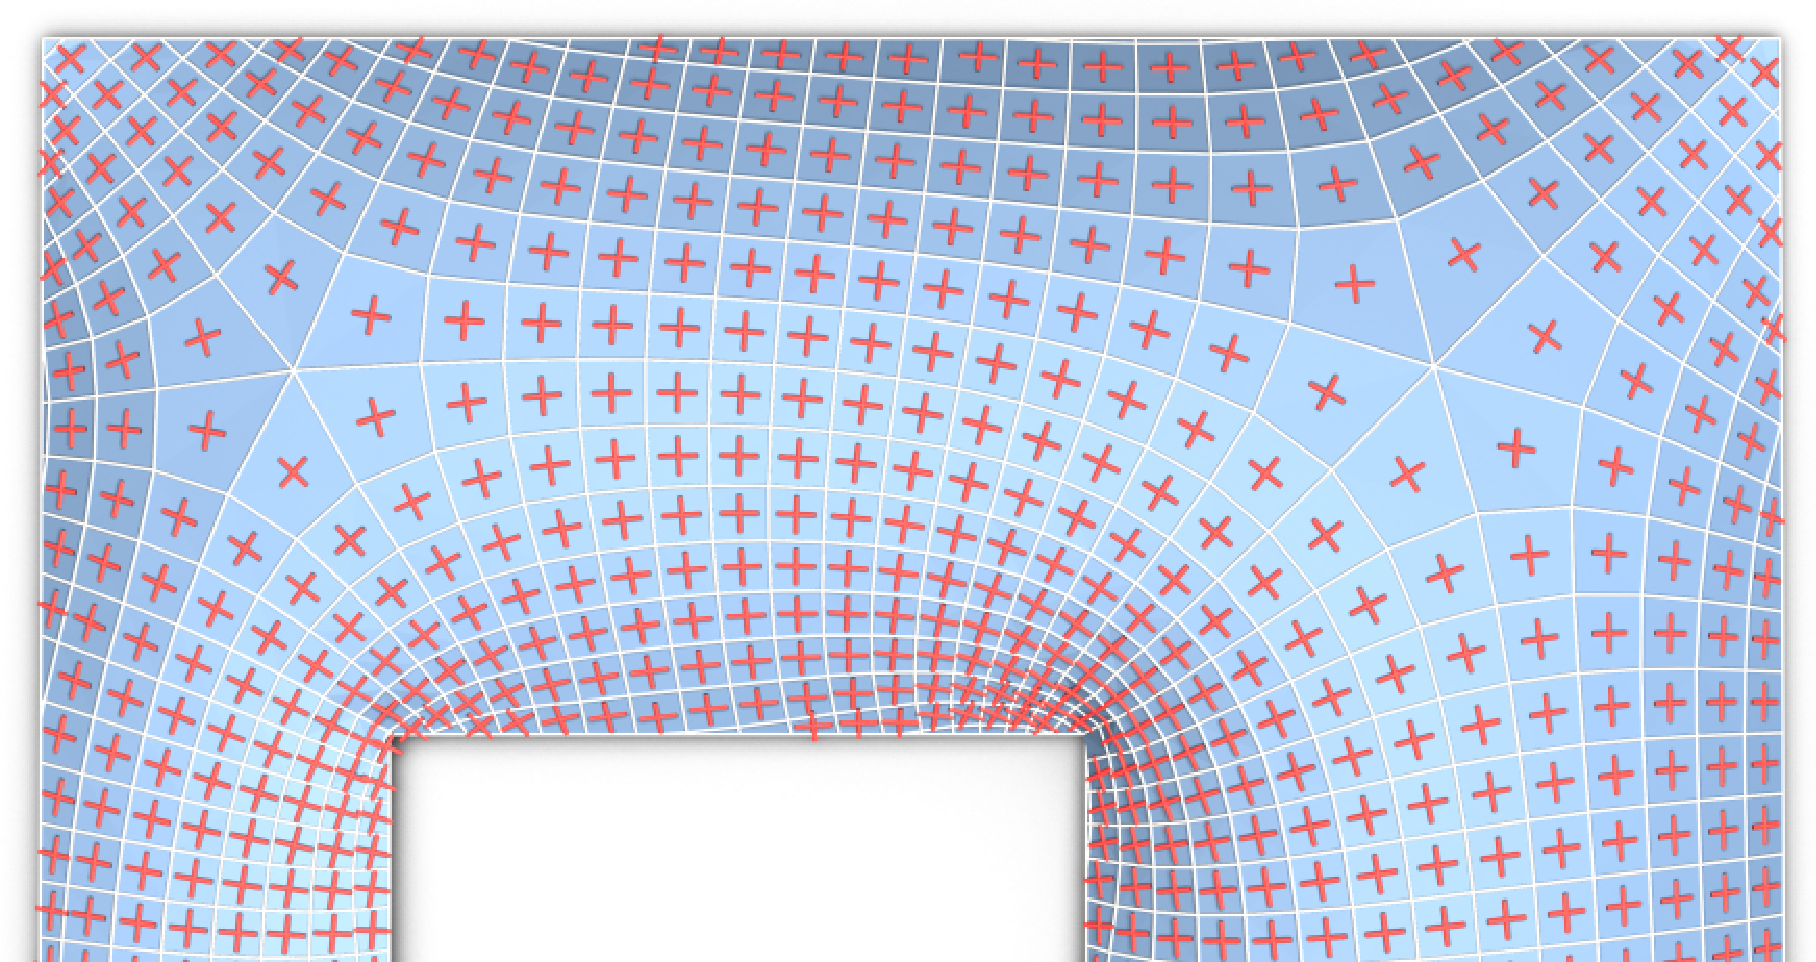
\includegraphics[width=\linewidth]{image/aag2012/dach_example01_directions.pdf}
\caption{Parameterization of the \textsc{Roof} model. The discrete 
curvature lines approximate curvature directions with high quality. See 
Section~\ref{subsub:examples_quality} for a discussion.}
\label{fig:dach01_directions}
\end{figure}

\subsubsection{Implementation}
\label{subsub:parameterization}

The algorithm to compute a quasiisothermic parameterization with vanishing modulus at the 
boundary of the domain is the following:
\begin{compactenum}[(1)]
\item Generate curvature directions and compute $\alpha$ at the boundary
\item Calculate boundary angles $\theta$ and pick singularities
\item Compute conformal parameterization with given $\theta$s
\item Perform remeshing
\item Remove cone point cuts 
\end{compactenum}

To estimate principle curvature fields we use the method of Cohen-Steiner and
Morvan \cite{CohMor03}, where the curvature tensor is averaged over a disk of a
given radius centered at edge midpoints. Together with a fixed orientation
of the surface this defines the angle function
$\alpha$. 

We deduce the angles $\theta$ for the boundary vertices as described in
Section~\ref{subsub:boundary}. These angles are the boundary curvatures we plug
into the algorithm of Springborn \emph{et al.}\ to obtain a conformal
parameterization. If necessary, we pick singularities for the curvature field at vertices
and prescribe corresponding cone angles by inspection of the curvature direction
field on the interior of the surface. A consistent singularity choice can
easily be checked using Equation~(\ref{eq:gauss-bonnet}). By construction we 
can only process curvature fields with isolated singularities.

We layout the new edges in the parameter plane such that an arbitrary 
boundary edge $\Phi(\mathrm{\it{ij}})$ intersects the $v$-axis in the desired angle 
$\alpha_{\mathrm{\it{ij}}}$. By construction
the intersection angles coincide with the prescribed $\alpha$'s for all
boundary edges. 
The domain of parameterization can contain singularities, which are
modeled as cone points with prescribed curvature. Therefore we have to 
cut along paths from the cone points to the boundary of the mesh. 
The layout overlaps if singularities with negative curvature are used. 
To create seamless parameter lines we use the rectification approach 
described by Springborn~\emph{et~al.}~\cite{Springborn2008}.

Finally, we create a new mesh based on a regular $(u,v)$-grid in $\mathbb R^2$. 
The remeshing process is carried out as a subdivision step followed by some cleanup
and regluing: We use the projective interpolation in the texture domain to 
increase the quality of the result. Previously cut paths from singularities to the 
boundary are sewed up to obtain the final remesh.

\subsubsection{Examples and quality}
\label{subsub:examples_quality}

\begin{figure}
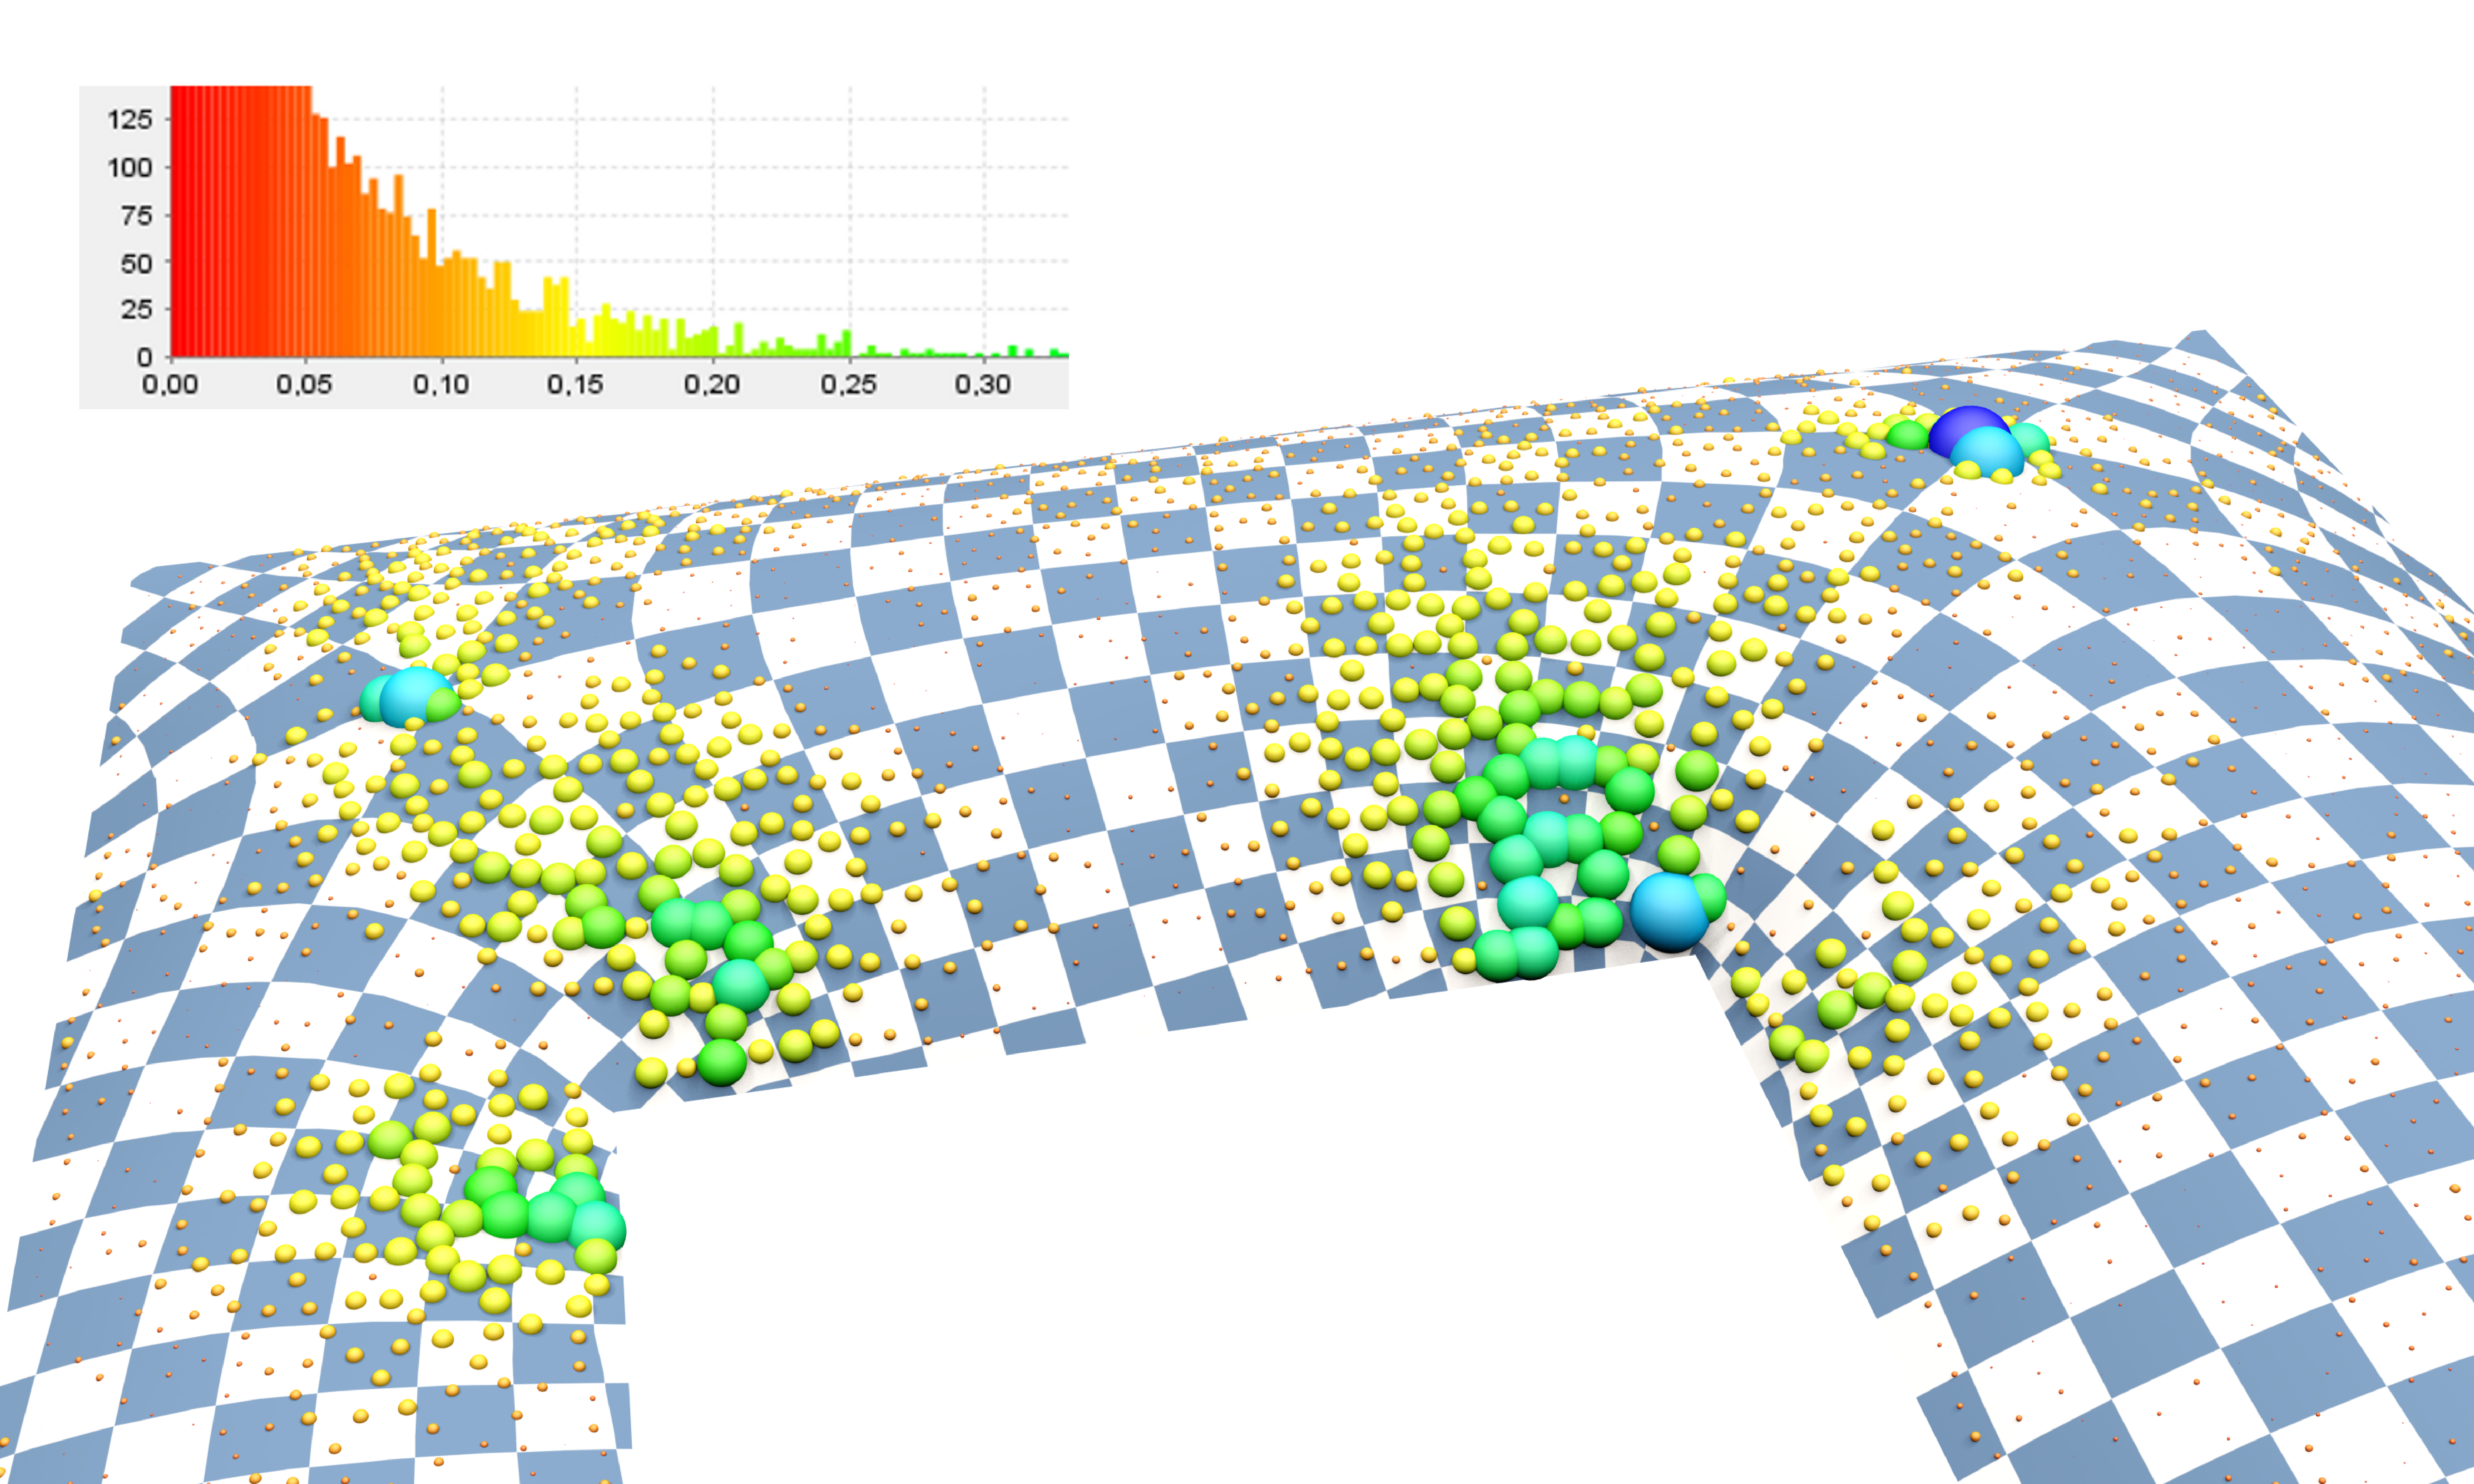
\includegraphics[width=\linewidth]{image/aag2012/dach01_quality_highres.pdf}
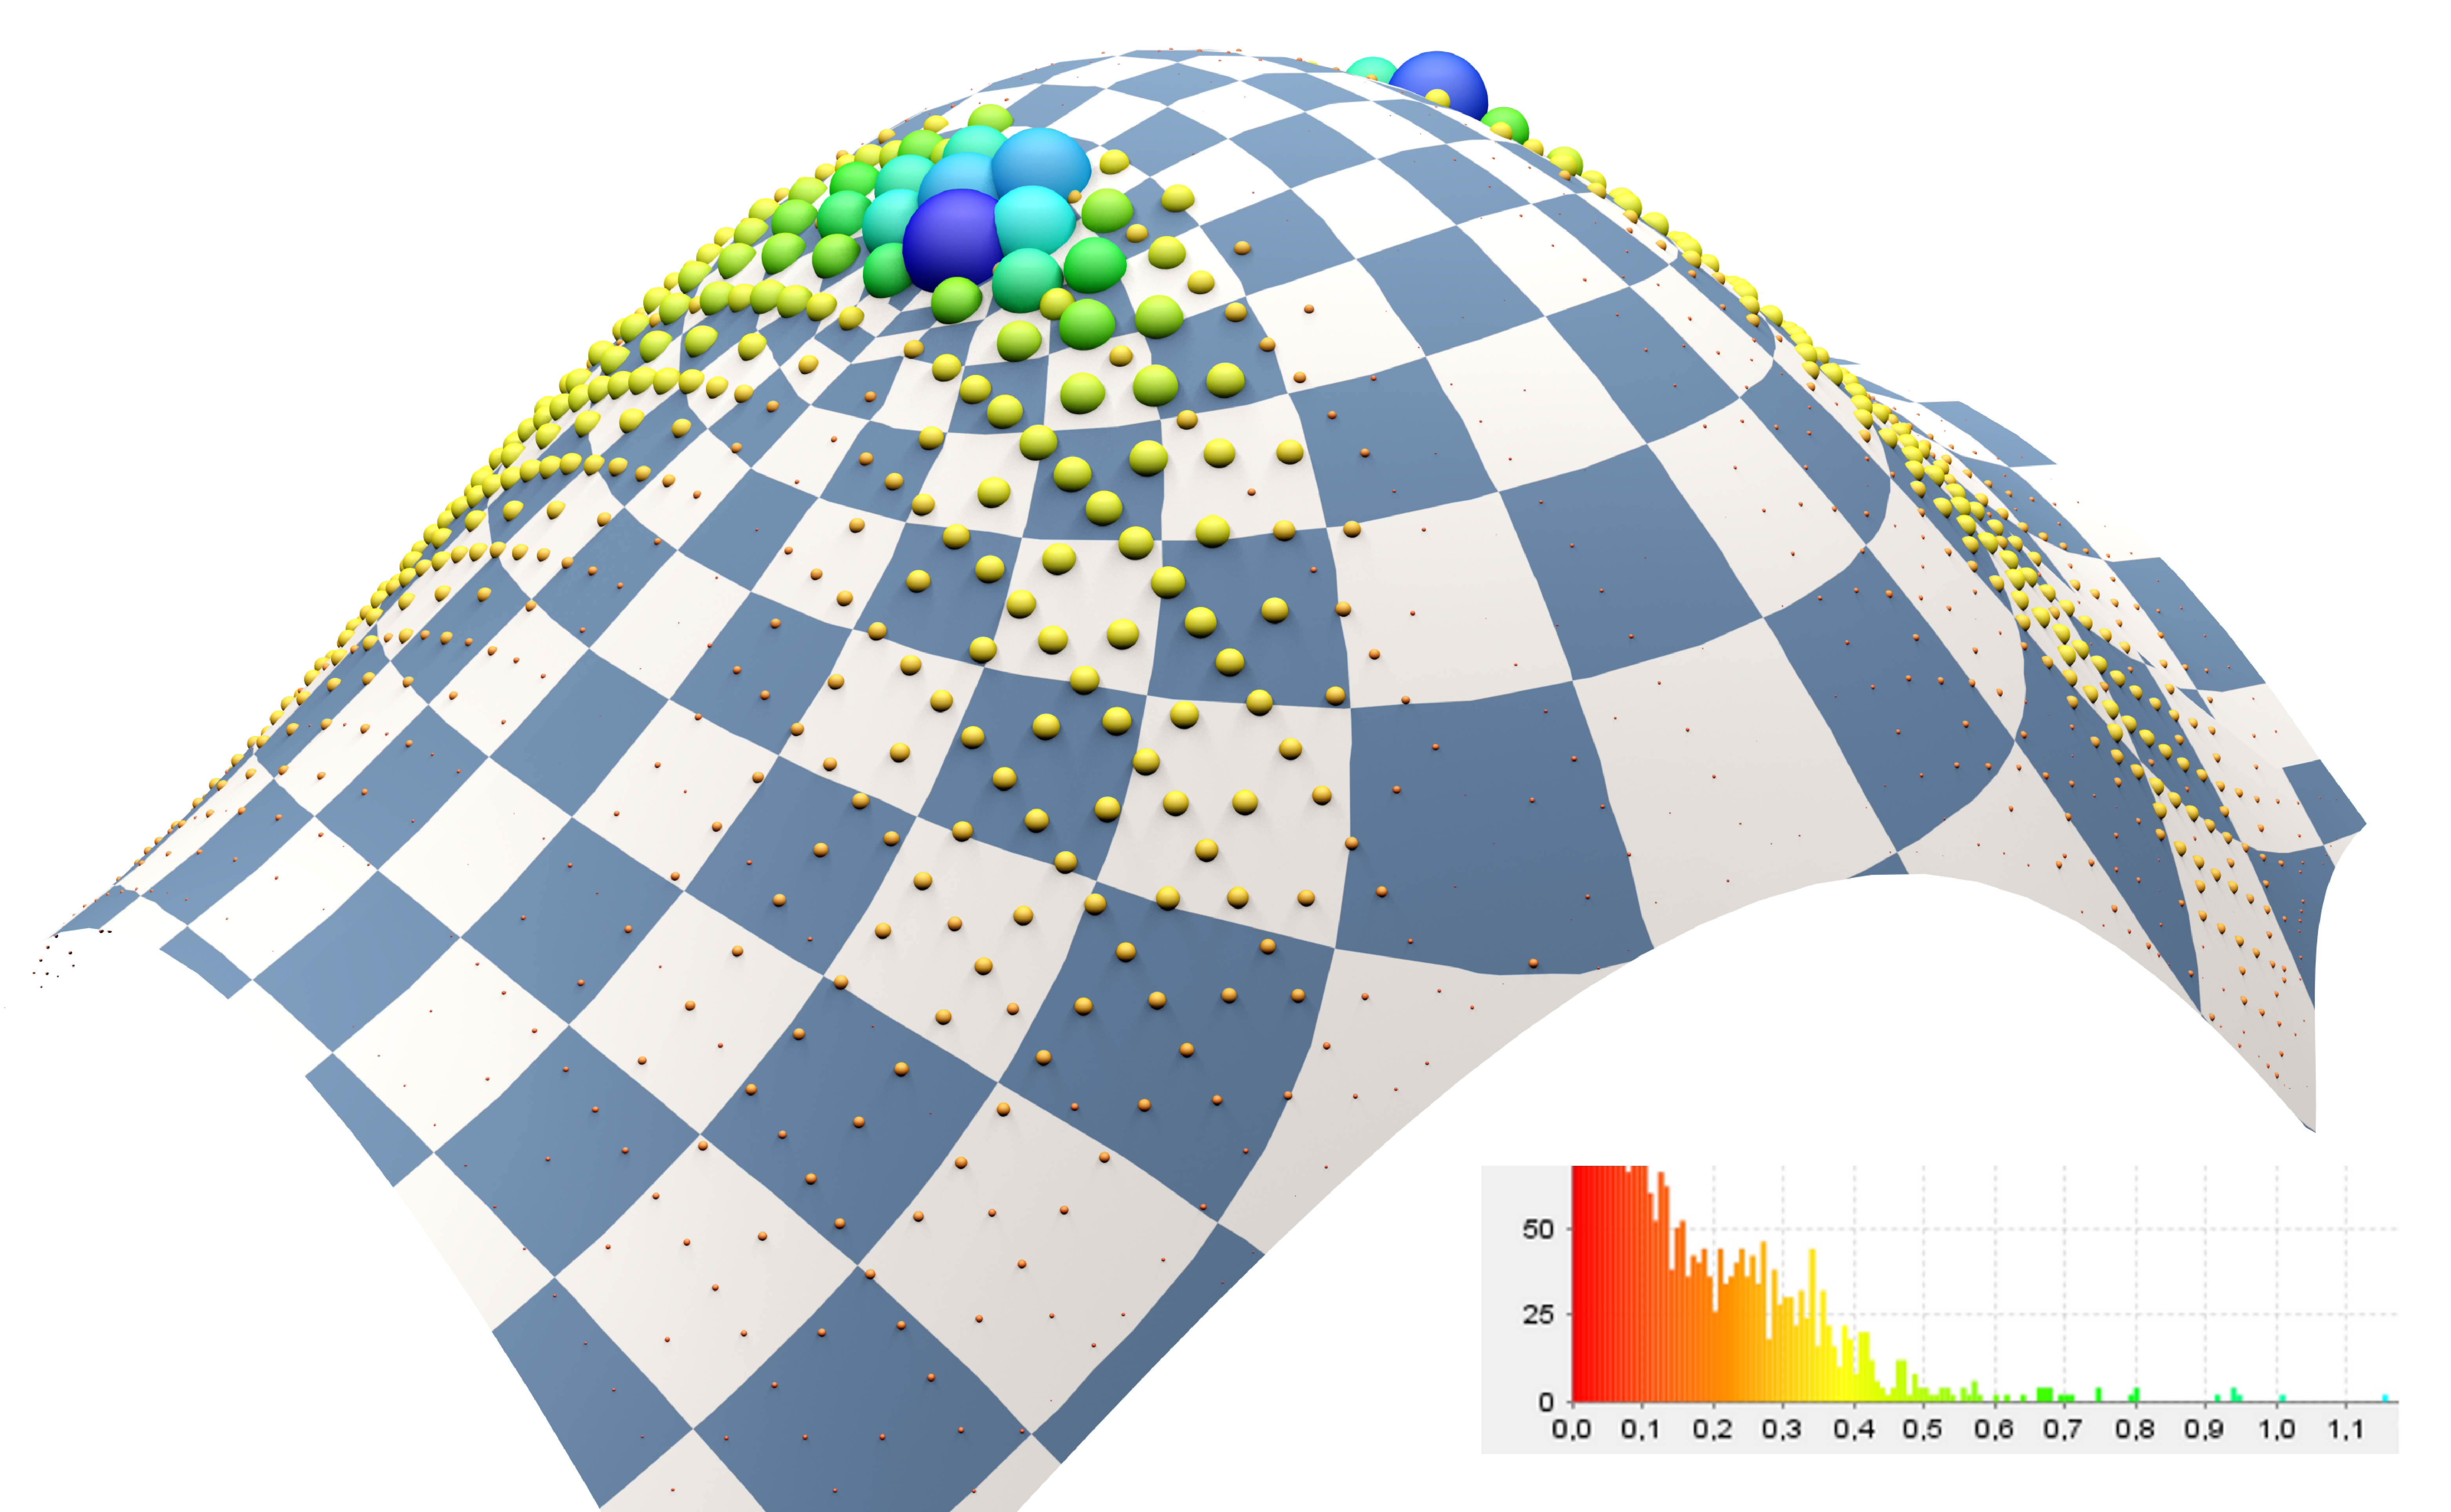
\includegraphics[width=\linewidth]{image/aag2012/dach02_quality_highres.pdf}
\caption[Parameterization quality plot]{The quality of the parameterization is measured in radians per
edge of the underlying triangulation. The checkerboard texture indicates the parameter
lines of the map. Small (red and yellow) beads represent good curvature direction quality, big
beads (green and blue) represent high deviation. The color of the histogram
corresponds to the color of the beads. Note that the mean error of the \textsc{Roof} 
surface (top) is half the error of the \textsc{Dome}. See also Table~\ref{tab:quality} 
for detailed quality measures of the other surfaces.}
\label{fig:quality}
\end{figure}
With the quasiisothermic modulus~$Q^\alpha$ on edges introduced in
Equation~(\ref{eq:quasiisothermicity}) we are now able to measure the 
quality of our parameterizations. 


There are two kinds of examples to consider: The first class of meshes stems from
smooth surfaces that admit conformal curvature line parameterizations, i.e.,
triangulations approximating isothermic surfaces. The second class consists of
arbitrary non-isothermic surfaces. For almost isothermic surfaces we expect
our parameterization to reconstruct the isothermic coordinates up to numerical
precision and hence $Q^\alpha$ to be reasonably small. For non-isothermic
surfaces we achieve the correct directions on the boundary but lack accuracy in
the interior. In Table~\ref{tab:quality} we summarize the numerical results
obtained from the surfaces of Figure~\ref{fig:all_mesh}.

\bigskip
\noindent \textbf{Isothermic surfaces.} The class of smooth isothermic
surfaces contains surfaces of constant mean curvature, surfaces of revolution,
and conic sections.  We use the \textsc{Minimal} example as an instance of an 
isothermic surface with mean curvature zero (Figure~\ref{fig:all_mesh}b). 
As expected this surface exhibits the highest curvature line quality of all tested 
meshes. The error however cannot vanish completely since the surface's curvature 
field contains singularities. In the vicinity of these points the numerical curvature 
directions contain significant amounts of noise.

\bigskip
\noindent \textbf{Non-isothermic surfaces.} Non-isothermic surfaces are
surfaces that do not admit a parameterization with conformal curvature lines. We
investigate
the properties of surfaces (a), (c), and (d) displayed in
Figure~\ref{fig:all_mesh}.

\begin{table}
\centering
\begin{tabular*}{0.7\linewidth}{l|l|l|l|l|l}
 & $\#E$ & $\#\partial E$ & $Q^\alpha_{\mathrm{mean}}$ & $Q^\alpha_{\mathrm{max}}$ &
$Q^\alpha_{\mathrm{\sigma}}$ \\ \hline
\textsc{Minimal} & 6260 & 450 & 0.036 & 0.603 & 0.033\\
\textsc{Teaser} & 17550 & 1000 & 0.057 & 1.20 & 0.066\\
\textsc{Roof} & 3766 & 470 & 0.051 & 0.610 & 0.059 \\
\textsc{Dome} & 1900 & 350 & 0.133 & 1.52 & 0.157
\end{tabular*}  
\caption{The curvature line approximation quality of the examples. $\#\partial
E$ are the number of boundary edges. $Q^\alpha_{\mathrm{\sigma}}$ is the standard
deviation of $Q^\alpha$.}
\label{tab:quality}
\end{table}

The \textsc{Teaser} surface was created as a minimizer of a spring functional
fixing the boundary and modelling interior edges as springs of rest length
zero. It is not far away from a minimal surface with the same boundary. The
curvature
line pattern however differs substantially as it contains singularities whereas
the minimal surface with this boundary curve does not. The quality of the
curvature line pattern is also very high. The mean angle error of the numerical
directions is $3.2$ degrees. Note that the deviation $Q_\sigma$ from the mean
value is also very low. For this surface the coordinates generated by our
algorithm are a globally good approximation to conformal curvature lines.

A quality plot of the \textsc{Roof} surface (Figures~\ref{fig:all_mesh}d and
\ref{fig:dach01_directions}) is shown in Figure~\ref{fig:quality}. Surprisingly, 
the quality of the curvature lines is as high as in the \textsc{Teaser} or the 
\textsc{Minimal} case. This suggests that a slight variation of the surface 
yields an isothermic surface. See also Figure~\ref{fig:dach01_directions} for 
a visual impression of the quality of the curvature lines.

The \textsc{Dome} model (Figure~\ref{fig:all_mesh}c) is created from a NURBS
surface. The quality plot (Figure~\ref{fig:quality}) reveals
areas of high angle deviation especially around the singularities. 
Other areas, in particular those near the boundary, are of high curvature line quality. 
The distance to the nearest isothermic surface is expected to be larger than in the
previous examples. More evidence for this is given in
Section~\ref{sec:s-isothermic}.

\bigskip
\noindent\textbf{Discussion.}
Our parameterization scheme works well for surfaces that are not too far away
from surfaces that possess isothermic coordinates. In the case of surfaces
stemming from minimal or constant mean curvature surfaces we get almost perfect
approximation quality of curvature lines. These are surfaces that are
particularly interesting when designing beam layouts for roof structures that
where form-found. For
other surfaces the parameterization is conformal and the parameter line pattern
captures the combinatorics of the curvature line pattern while approximating
the curvature line geometry.
There are of course surfaces for which our method is not applicable.
If the boundary is too short compared to the overall size of the surface we 
cannot expect the solution to follow curvature lines as the distance to the boundary 
increases.


\section{Discrete s-isothermic surfaces}
\label{sec:s-isothermic}

\begin{figure}
\centering
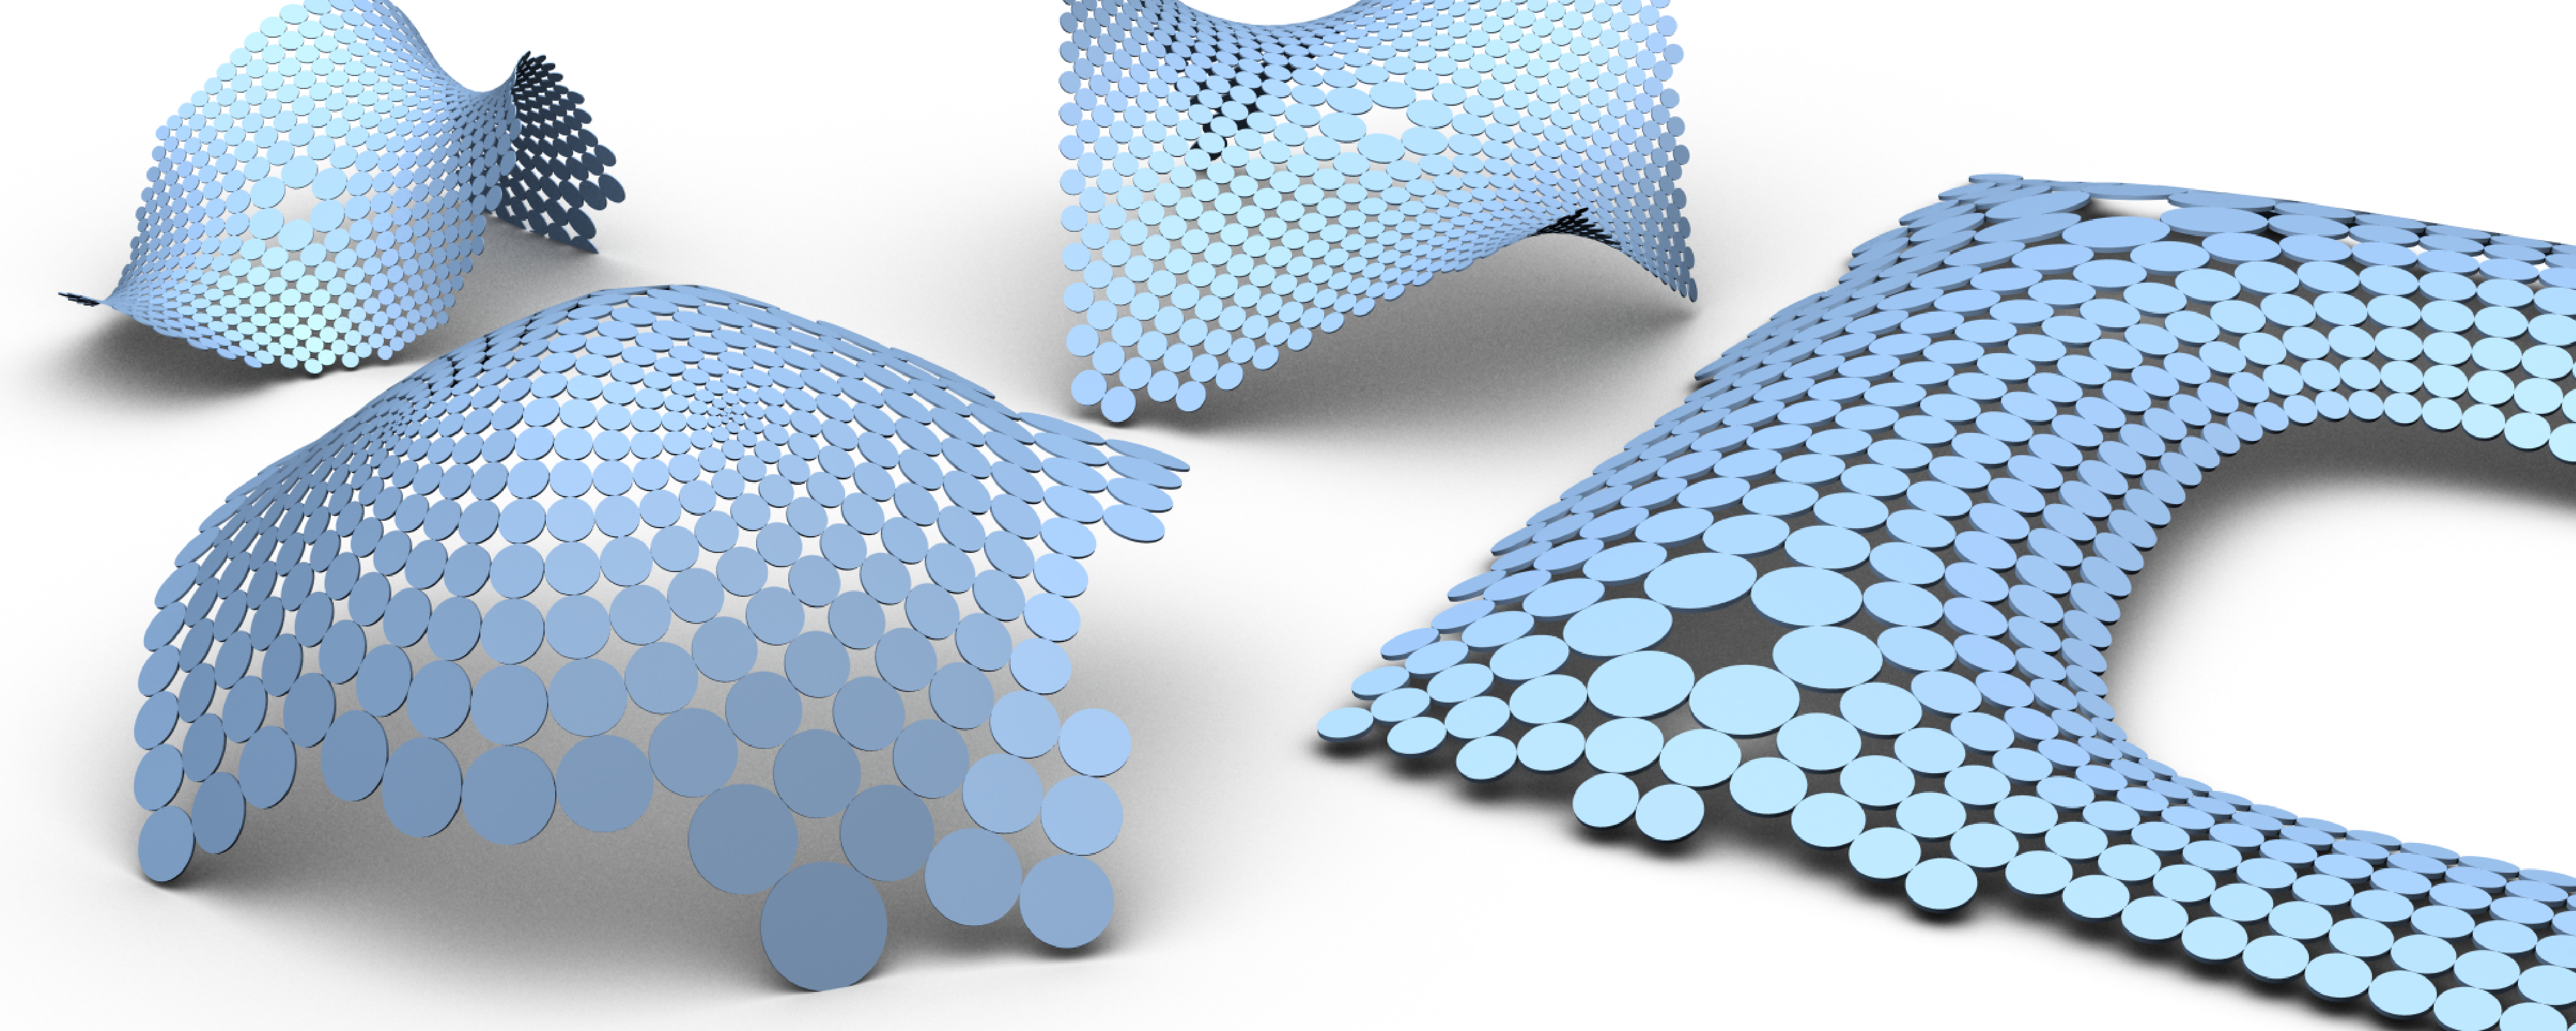
\includegraphics[width=\linewidth]{image/aag2012/all_circles.pdf}
\caption[S-isothermic meshes]{S-isothermic meshes created from the models presented in
Figure~\ref{fig:all_mesh}.
The inner quadrilaterals are optimized towards touching incircles. A series of
touching circles in a row can be interpreted as discrete curvature line.}
\label{fig:s_isothermic}
\end{figure}

Starting with a quasiisothermically parameterized mesh with low modulus 
we now aim to create discrete s-isothermic surfaces that
stay in the vicinity of the input surface. S-isothermic surfaces were
introduced by Bobenko and Pinkall~\cite{BobenkoP1996}: A quadrilateral mesh
is \mbox{\emph{s-isothermic}} if (i) all the quadrilaterals are planar, (ii)
all faces have incircles, and (iii) the incircles of adjacent quadrilaterals
touch.
Figure~\ref{fig:s_isothermic} displays s-isothermic surfaces derived from our
parametrizations shown in Figure~\ref{fig:all_mesh}.

\subsubsection{Variational Principle}

\begin{figure}
\centering
\resizebox{0.4\textwidth}{!}{\input{figures/e_touching_circles.pdf_t}}
\caption{Labels for the touching-circle
functional at an edge. The circles touch 
if the ratio $\cot\left(\beta^i/2\right)/\cot\left(\beta^j/2\right)$ is equal on both sides of the edge.}
\label{fig:functional}
\end{figure}

In this section we introduce an energy whose minimizers are s-isothermic
surfaces. We denote quadilaterals by $ijkm\in F$ where the indices are in 
cyclic order.
The s-isothermic energy $E_S$ consists of three parts:
\begin{equation}
  E_S := 
  \lambda_1 E_{\mathrm{planar}} + 
  \lambda_2 E_{\mathrm{incircle}} + 
  \lambda_3 E_{\mathrm{touch}}
\end{equation}
The planarity energy $E_{\mathrm{planar}}$ penalizes non-planar quadrilateral
faces. For each quad it can be defined either by the distance of the diagonals
(an idea attributed to Peter Schr\"oder~\cite{PottmannSBSWBW2008}) or the
volume of the tetrahedron spanned by the
four vertices. We give the formula for the former here. 
\begin{equation}
E_{\mathrm{planar}} = \sum_{\mathrm{\it{ijkm}} \in F} \frac{\left<\Delta_{\mathrm{\it{ji}}},\Delta_{\mathrm{\it{mj}}} \times \Delta_{\mathrm{\it{ki}}}\right>^2}
{\Vert\Delta_{\mathrm{\it{mj}}} \times \Delta_{\mathrm{\it{ki}}}\Vert^2}
\end{equation}
Here $\Delta_{ij}$ is the vector pointing from vertex $i$ to $j$.

For $E_{\mathrm{incircle}}$ we use the energy defined by Schiftner~\emph{et~al.}~\cite{SchiftnerHWP2009} based on the fact that the sum of opposite edge
lengths must be equal for a planar quad to possess an incircle.
\begin{equation}
E_{\mathrm{incircle}} = \sum_{\mathrm{\it{ijkm}} \in F} \left( l_{\mathrm{\it{ij}}} + 
l_{\mathrm{\it{km}}} - l_{\mathrm{\it{jk}}} - l_{\mathrm{\it{mi}}} \right)^2
\end{equation}
The energy
$E_{\mathrm{touch}}$ is a new energy that enforces touching incircles
if faces are planar and possess incircles.  It is defined per edge, see
Figure~\ref{fig:functional} for the exact labeling of the angles at one edge.
For an interior edge $ij\in E$ we define
\begin{equation}
  E_{\mathrm{touch}}(\mathrm{\it{ij}})=
  \left(\cot\frac{\beta^j_l}{2}\cot\frac{\beta^i_r}{2} - 
\cot\frac{\beta^j_r}{2}\cot\frac{\beta^i_l}{2}\right)^2.
\end{equation}
On boundary edges the energy is zero. All energies can be formulated 
in terms of the vertex coordinates and the derivatives can be calculated explicitly.

Since all energies are in general non-convex we need a good initial guess to 
find meaningful minimizers of $E_S$.
S-isothermic minimal surfaces converge to isothermic parameterizations of
smooth minimal surfaces~\cite{BobHofSpr06}. For general s-isothermic surfaces
this is an open conjecture. The parameterizations obtained in
Section~\ref{sec:parametrization} are good candidates to start from with the
optimization of the functional.
%numerics
We use the non-linear optimization package PETSc/TAO~\cite{petsc-web-page,
tao-user-ref} and its java binding~\cite{jpetsctao-web-page} to find
minimizers of $E_S$. Figure~\ref{fig:convergence} shows convergence plots of
$E_S$ for the four models that were discussed in the previous section.
\begin{figure}
\centering
\resizebox{\textwidth}{!}{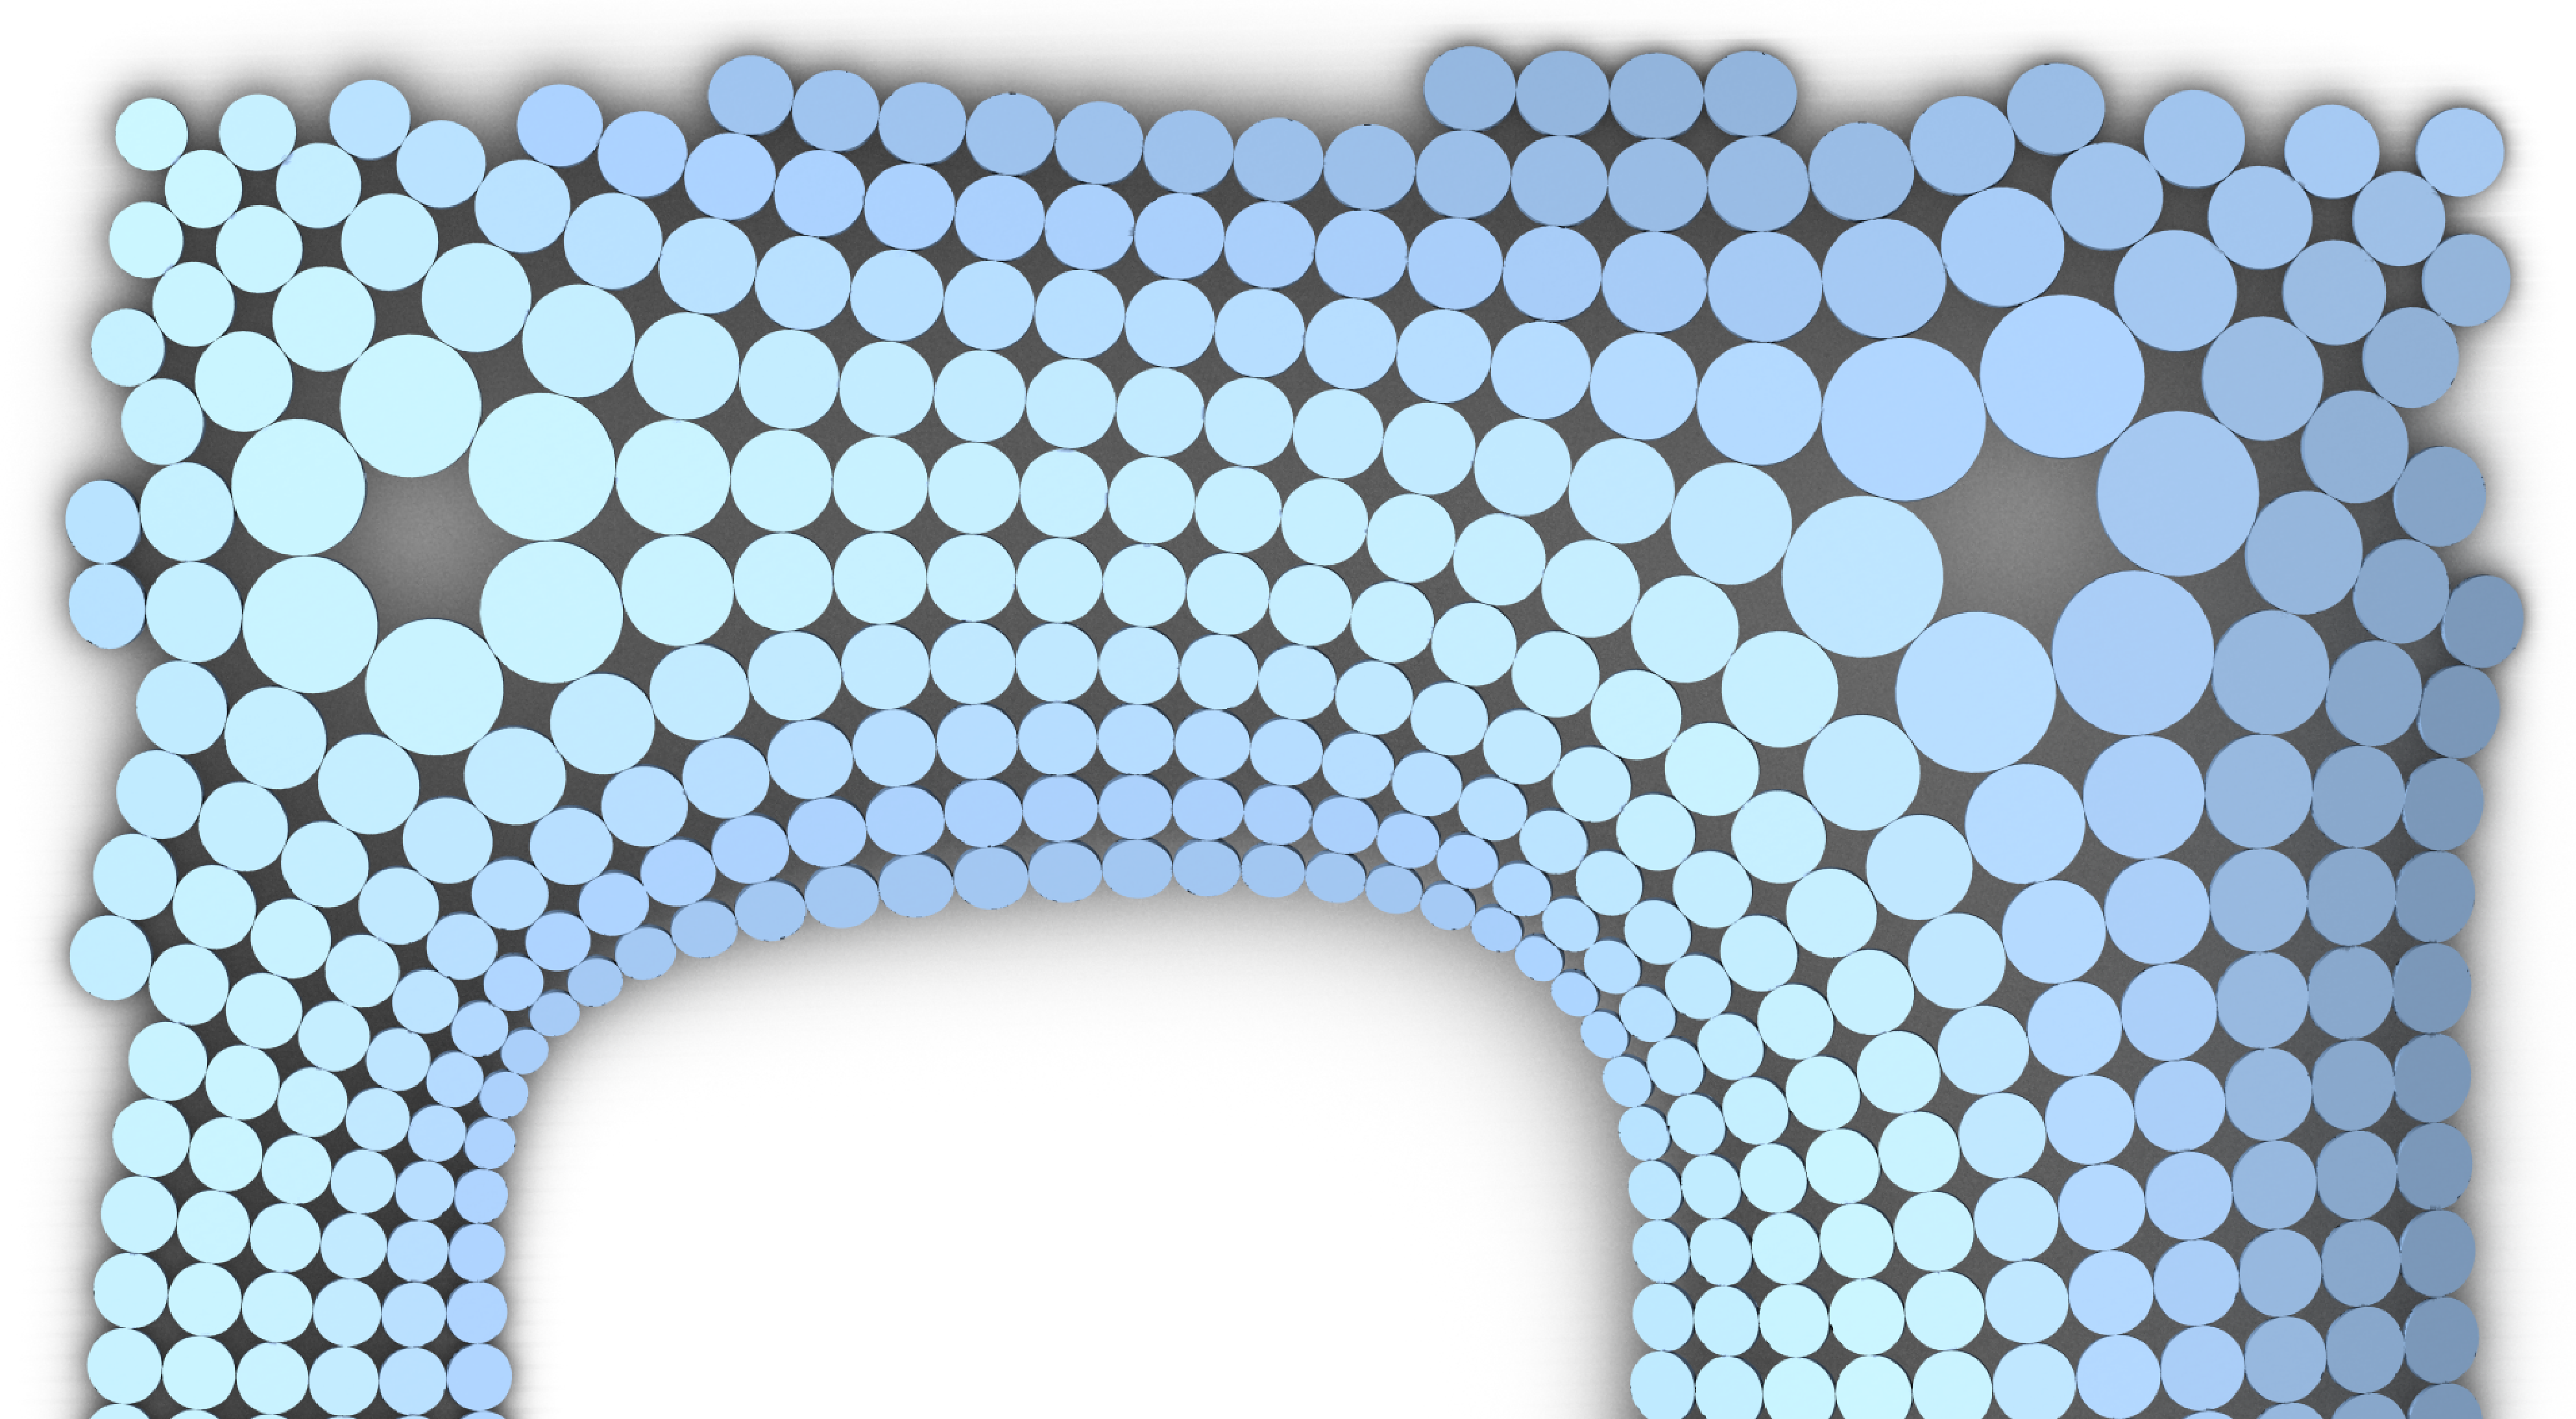
\includegraphics[width=\textwidth]{image/aag2012/dach_example01_circles.pdf}}
\caption{The s-isothermic circle packing on the \textsc{Roof} model in detail.}
\end{figure}

As seen in the quality analysis of Section~\ref{subsub:examples_quality}, the
\textsc{Teaser}, the \textsc{Minimal}, and the \textsc{Roof} models are
quasiisothermic surfaces with low modulus. For these models the corresponding s-isothermic
surface is also close to the input surface. Figure~\ref{fig:convergence} shows
the energy during the optimization. Here the three close-to-isothermic meshes
start with a lower energy than the \textsc{Dome} model. After the \textsc{Dome}
has passed some iterations it exhibits convergence properties similar to the
other models. As this surface converges against a discrete s-isothermic surface,
we observe a considerable change in shape during the first iterations
especially around the singularities.

\begin{figure}
\centering
\resizebox{0.7\textwidth}{!}{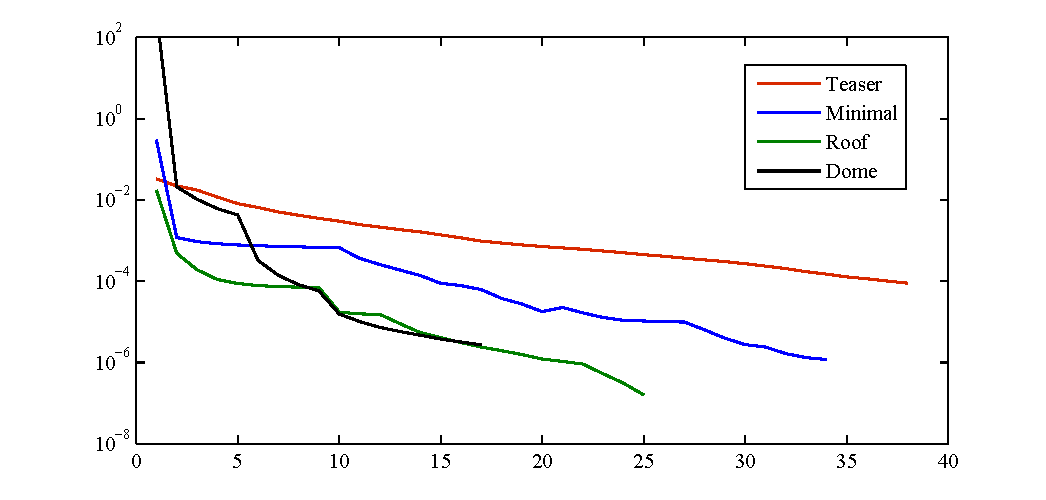
\includegraphics{image/aag2012/convergence_plots_embedded.pdf}}
\caption[Convergence behavior of $E_S$]{Convergence behavior of $E_S$ during optimization. We use the meshes 
displayed in Figure~\ref{fig:all_mesh} as initial guesses for the minimization. The
convergence of the Teaser geometry is slower due to the high complexity.}
\label{fig:convergence}
\end{figure}

\subsubsection{Isometric Deformations of Minimal Surfaces}
\label{sub:isometric}
\begin{figure*}
\centering
\resizebox{\textwidth}{!}{\input{figures/isometric.pdf_t}}
\caption{Non-trivial isometric deformations of a minimal surface. The edges of the dual
surface are rotated to create a \mbox{$1$-parameter} family of isometrically
deformed surfaces with 
period $2\pi$. The histogram shows the edge length error of the $90^\circ$ model
when compared 
with the initial surface. The mean edge length deviation of this model is $1.28\%$.}
\label{fig:isometric} 
\end{figure*}

Every smooth minimal surface possesses a $1$-parameter (associated) family of
non-trivial isometric deformations. All surfaces in this family have the same
Gau{\ss} map. For discrete s-isothermic minimal surfaces this construction is
discretized by Bobenko~\emph{et~al.}~\cite{BobHofSpr06}: Edge lengths and the conformality of the
parameterization are preserved. We need to introduce the concept of dual surface
to construct the family of isometric surfaces.

\noindent\textbf{The Dual Surface.}
In differential geometry for isothermic surfaces there is a notion of a dual
surface.  This dual or Christoffel transform is also an isothermic surface. Both
surfaces are parameterized with isothermic coordinates. This setup can be
discretized using the definition of discrete s-isothermic surfaces. The dual
surface can be constructed using the incircle structure of s-isothermic meshes.
We introduce consistent signs on edges on a discrete s-isothermic surface such
that opposite sides of the quads have the same sign and consecutive edges in a
quad have different signs. The dual mesh of a mesh $M$ will have parallel edges
calculated as follows: Let $e_{ij}=v_j-v_i$ be an edge vector of~$M$. Then the
dual edge vector $e_{ij}^*$ satisfies the following equation:
\[e_{ij}^* = \pm \frac{1}{r_i \cdot r_j} e_{ij}\]
where $r_i$ and $r_j$ are the distances from the vertex $v_i$ and $v_j$ to the
touching point of the incircles of incident faces at the edge~$e_{ij}$. For a
given
discrete s-isothermic mesh we can easily calculate the dual mesh by enumerating
the vertices along a spanning tree of edges. In Figure~\ref{fig:isometric} the
dual surface of the \textsc{Minimal} model is shown in the upper left hand
corner.  Via the dual surface we can now construct isometric deformations of
minimal surfaces.

\noindent\textbf{Deformation.}
The dual of a smooth minimal surface coincides with its Gau{\ss} map which is a
part of a sphere. This sphere may be multiply covered. For discrete s-isothermic
minimal surfaces this Gau{\ss} map is a part of a Koebe polyhedron, i.e., a
polyhedral surfaces with edges tangent to a sphere. On the Koebe polyhedron
every edge is rotated by a fixed angle in the tangent space of the sphere at the
points of tangency of the edge. The resulting edge vectors again form closed
quads and can be dualized. This dual surface has the same edge lengths as the
initial minimal surface.

For minimal quad meshes with touching incircles that were created using our
parameterization and the optimization step, the dual surface will be close to a
Koebe polyhedron. We use a least-squares-sphere to define a consistent tangent
space at the touching points of incircles with the edges. The resulting
deformation of a given minimal surface is then close to isometric. To distribute
the isometry error on the edges we average over different roots of the layout
spanning tree. Surfaces that do not possess exact isometric deformations are
deformed approximative.

We apply this procedure to the \textsc{Minimal} model
\mbox{(Figure~\ref{fig:all_mesh}a)}. Figure~\ref{fig:isometric} shows the
surface together
with its dual and isometrically deformed versions with different turning angles.

\section{A discrete s-isothermic ellipsoid and its dual surface}
\label{sec:discrete_ellipsoid}

\begin{figure*}
\centering
\resizebox{\textwidth}{!}{
$\vcenter{\hbox{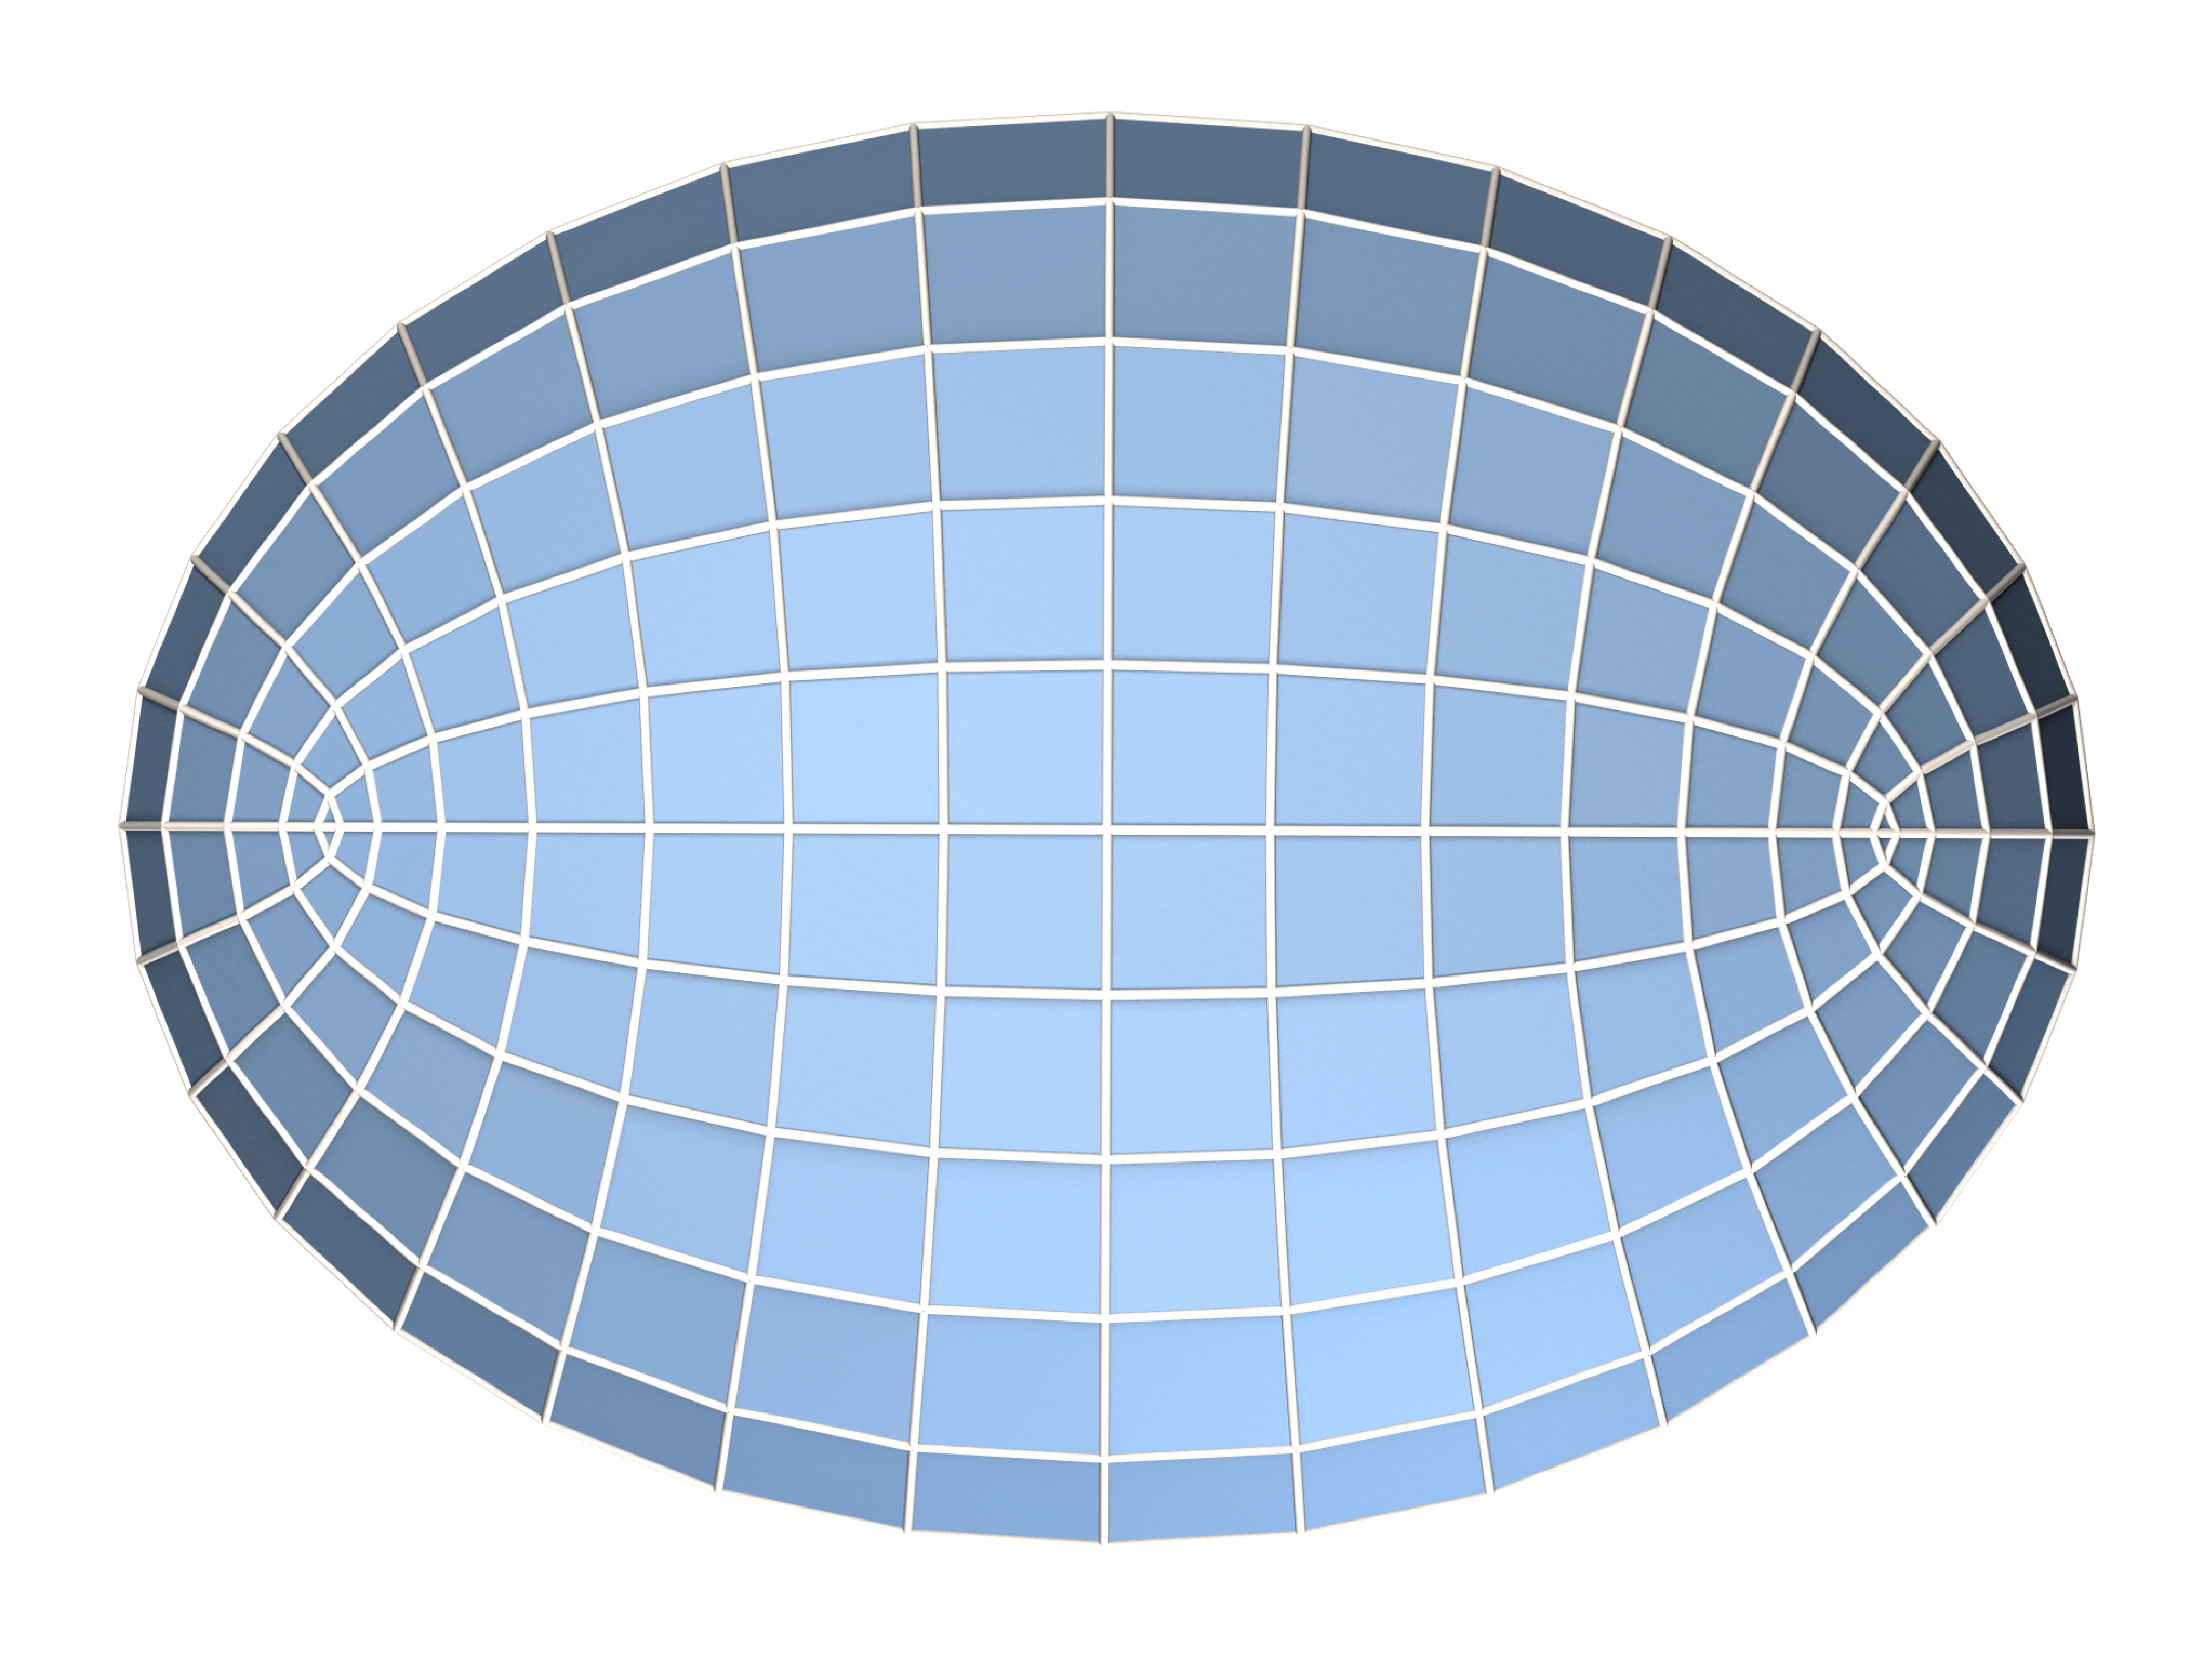
\includegraphics[width=0.5\textwidth]{image/ellipsoid01_top.pdf}}}$
$\vcenter{\hbox{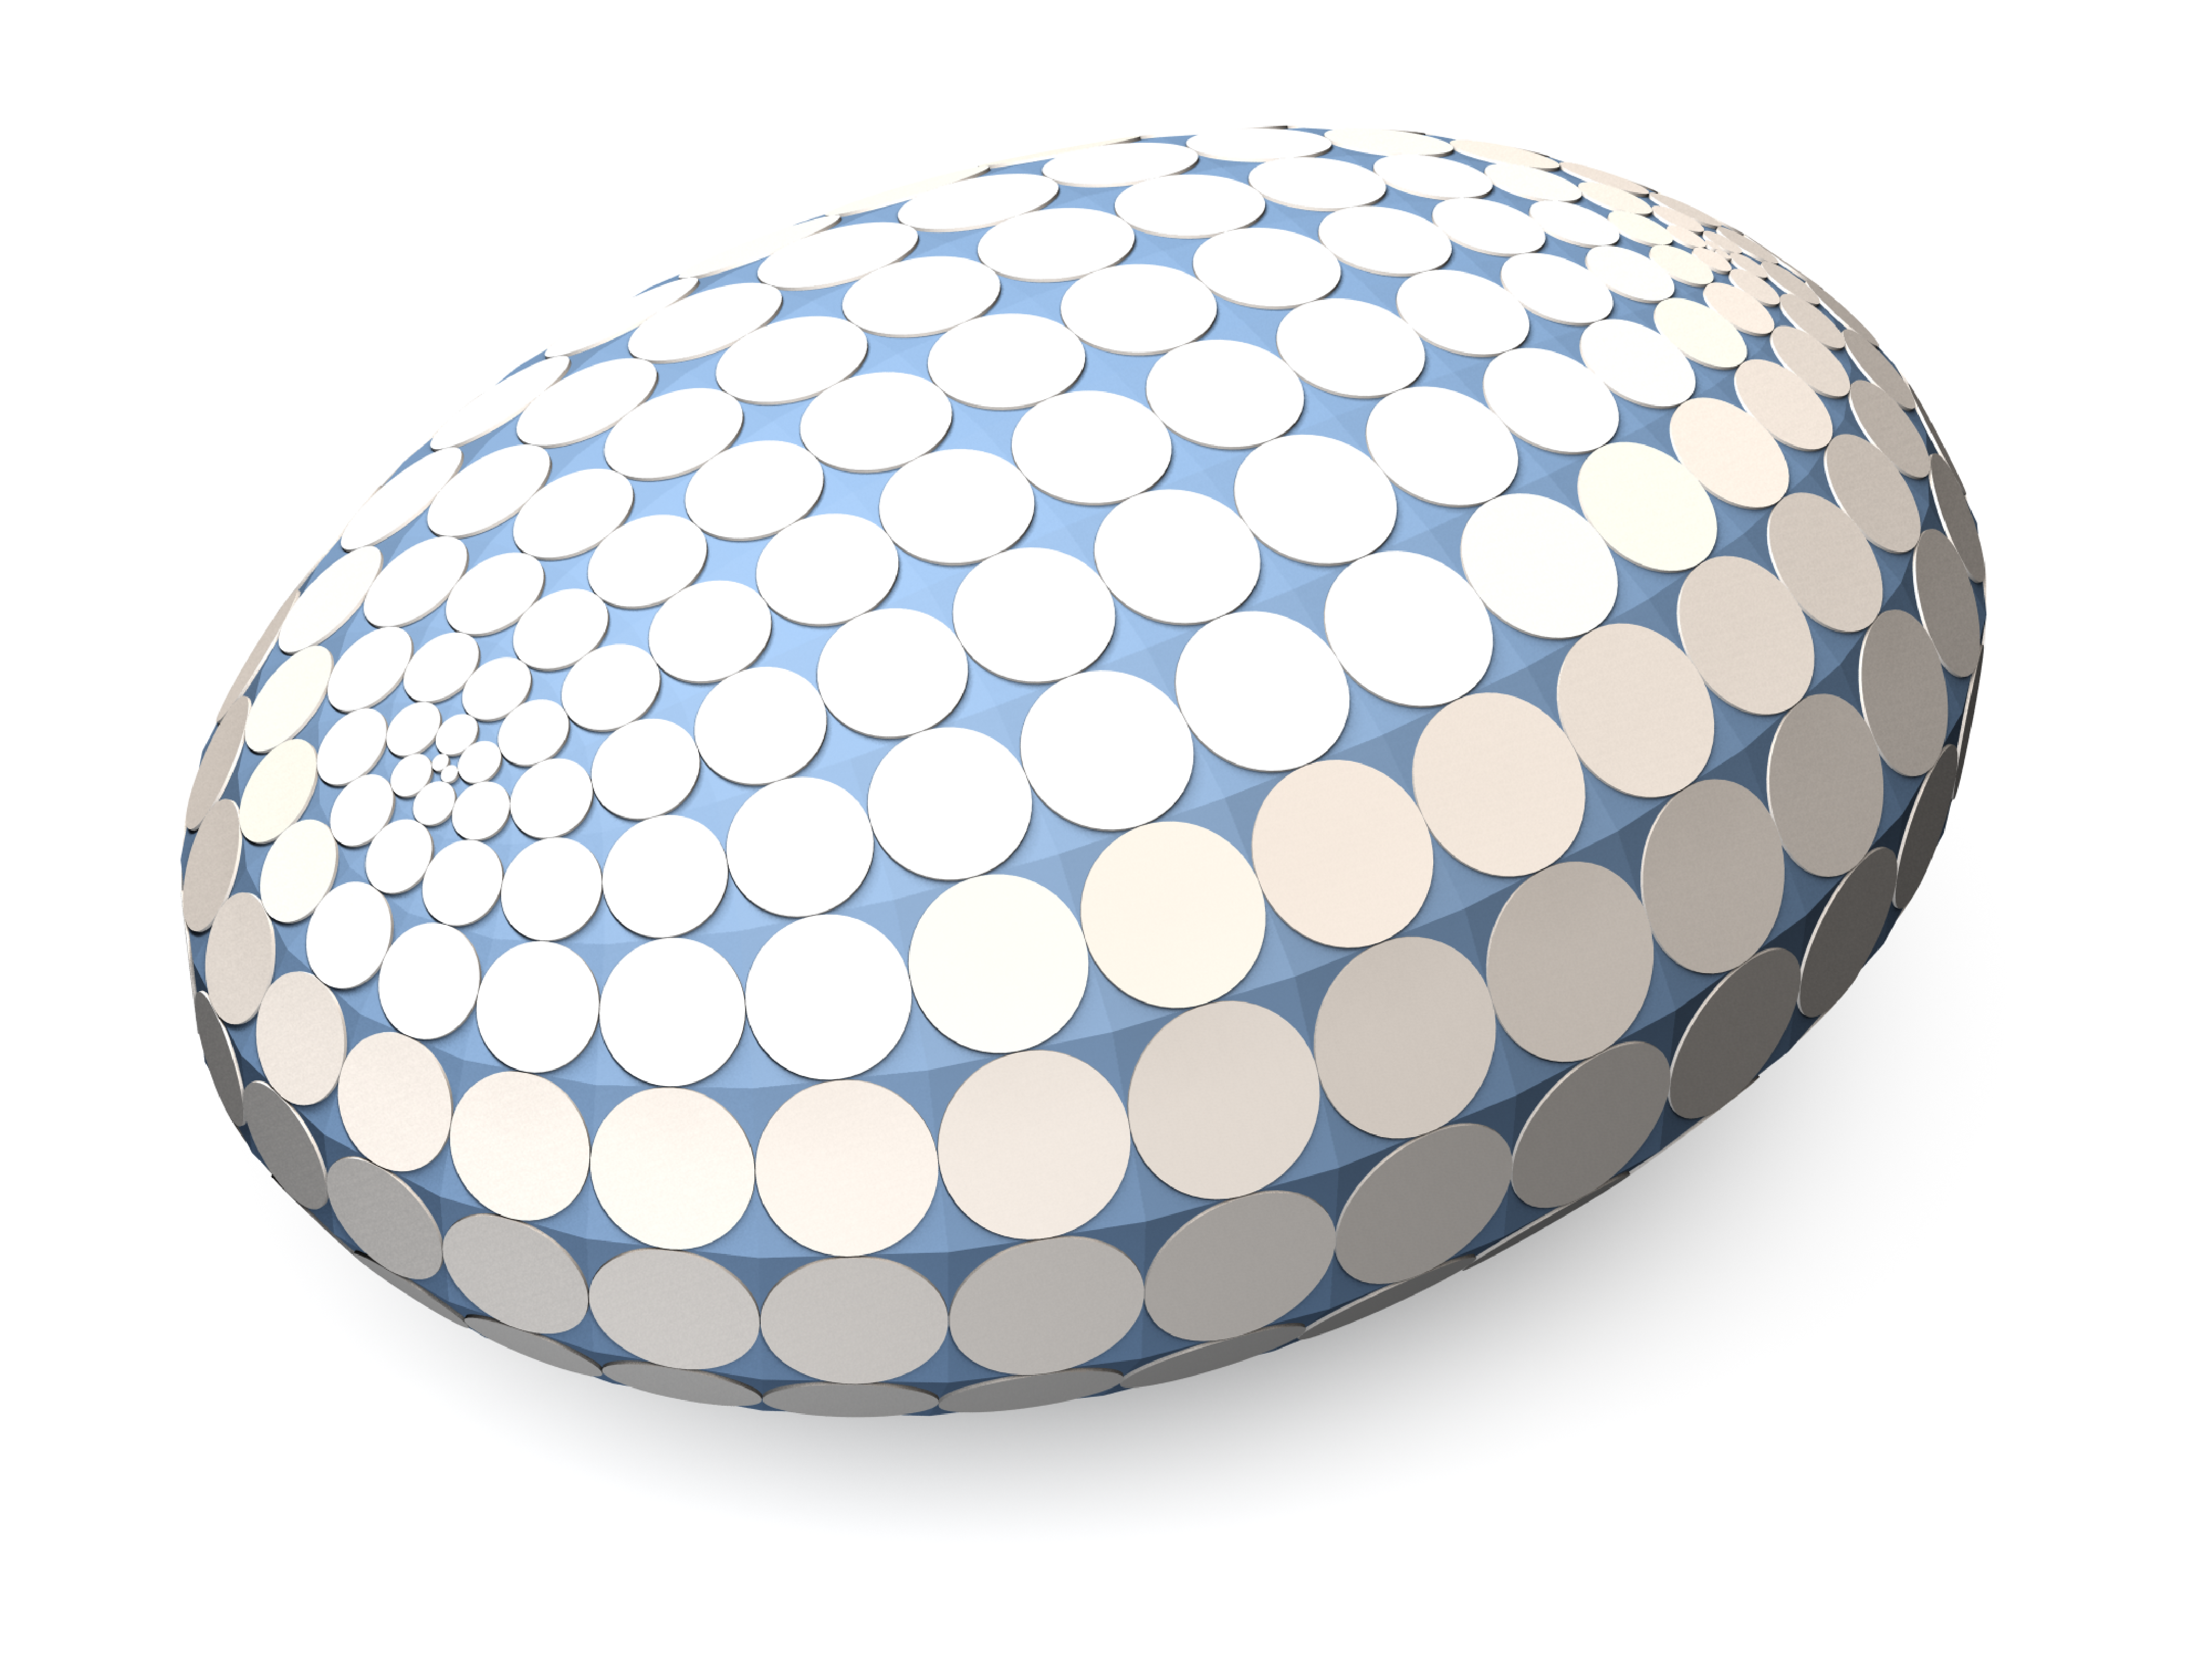
\includegraphics[width=0.5\textwidth]{image/ellipsoid01_disks.pdf}}}$
}
\caption{Discrete s-isothermic ellipsoid}
\label{fig:ellipsoid} 
\end{figure*}

\begin{figure}
\centering
\resizebox{\textwidth}{!}{
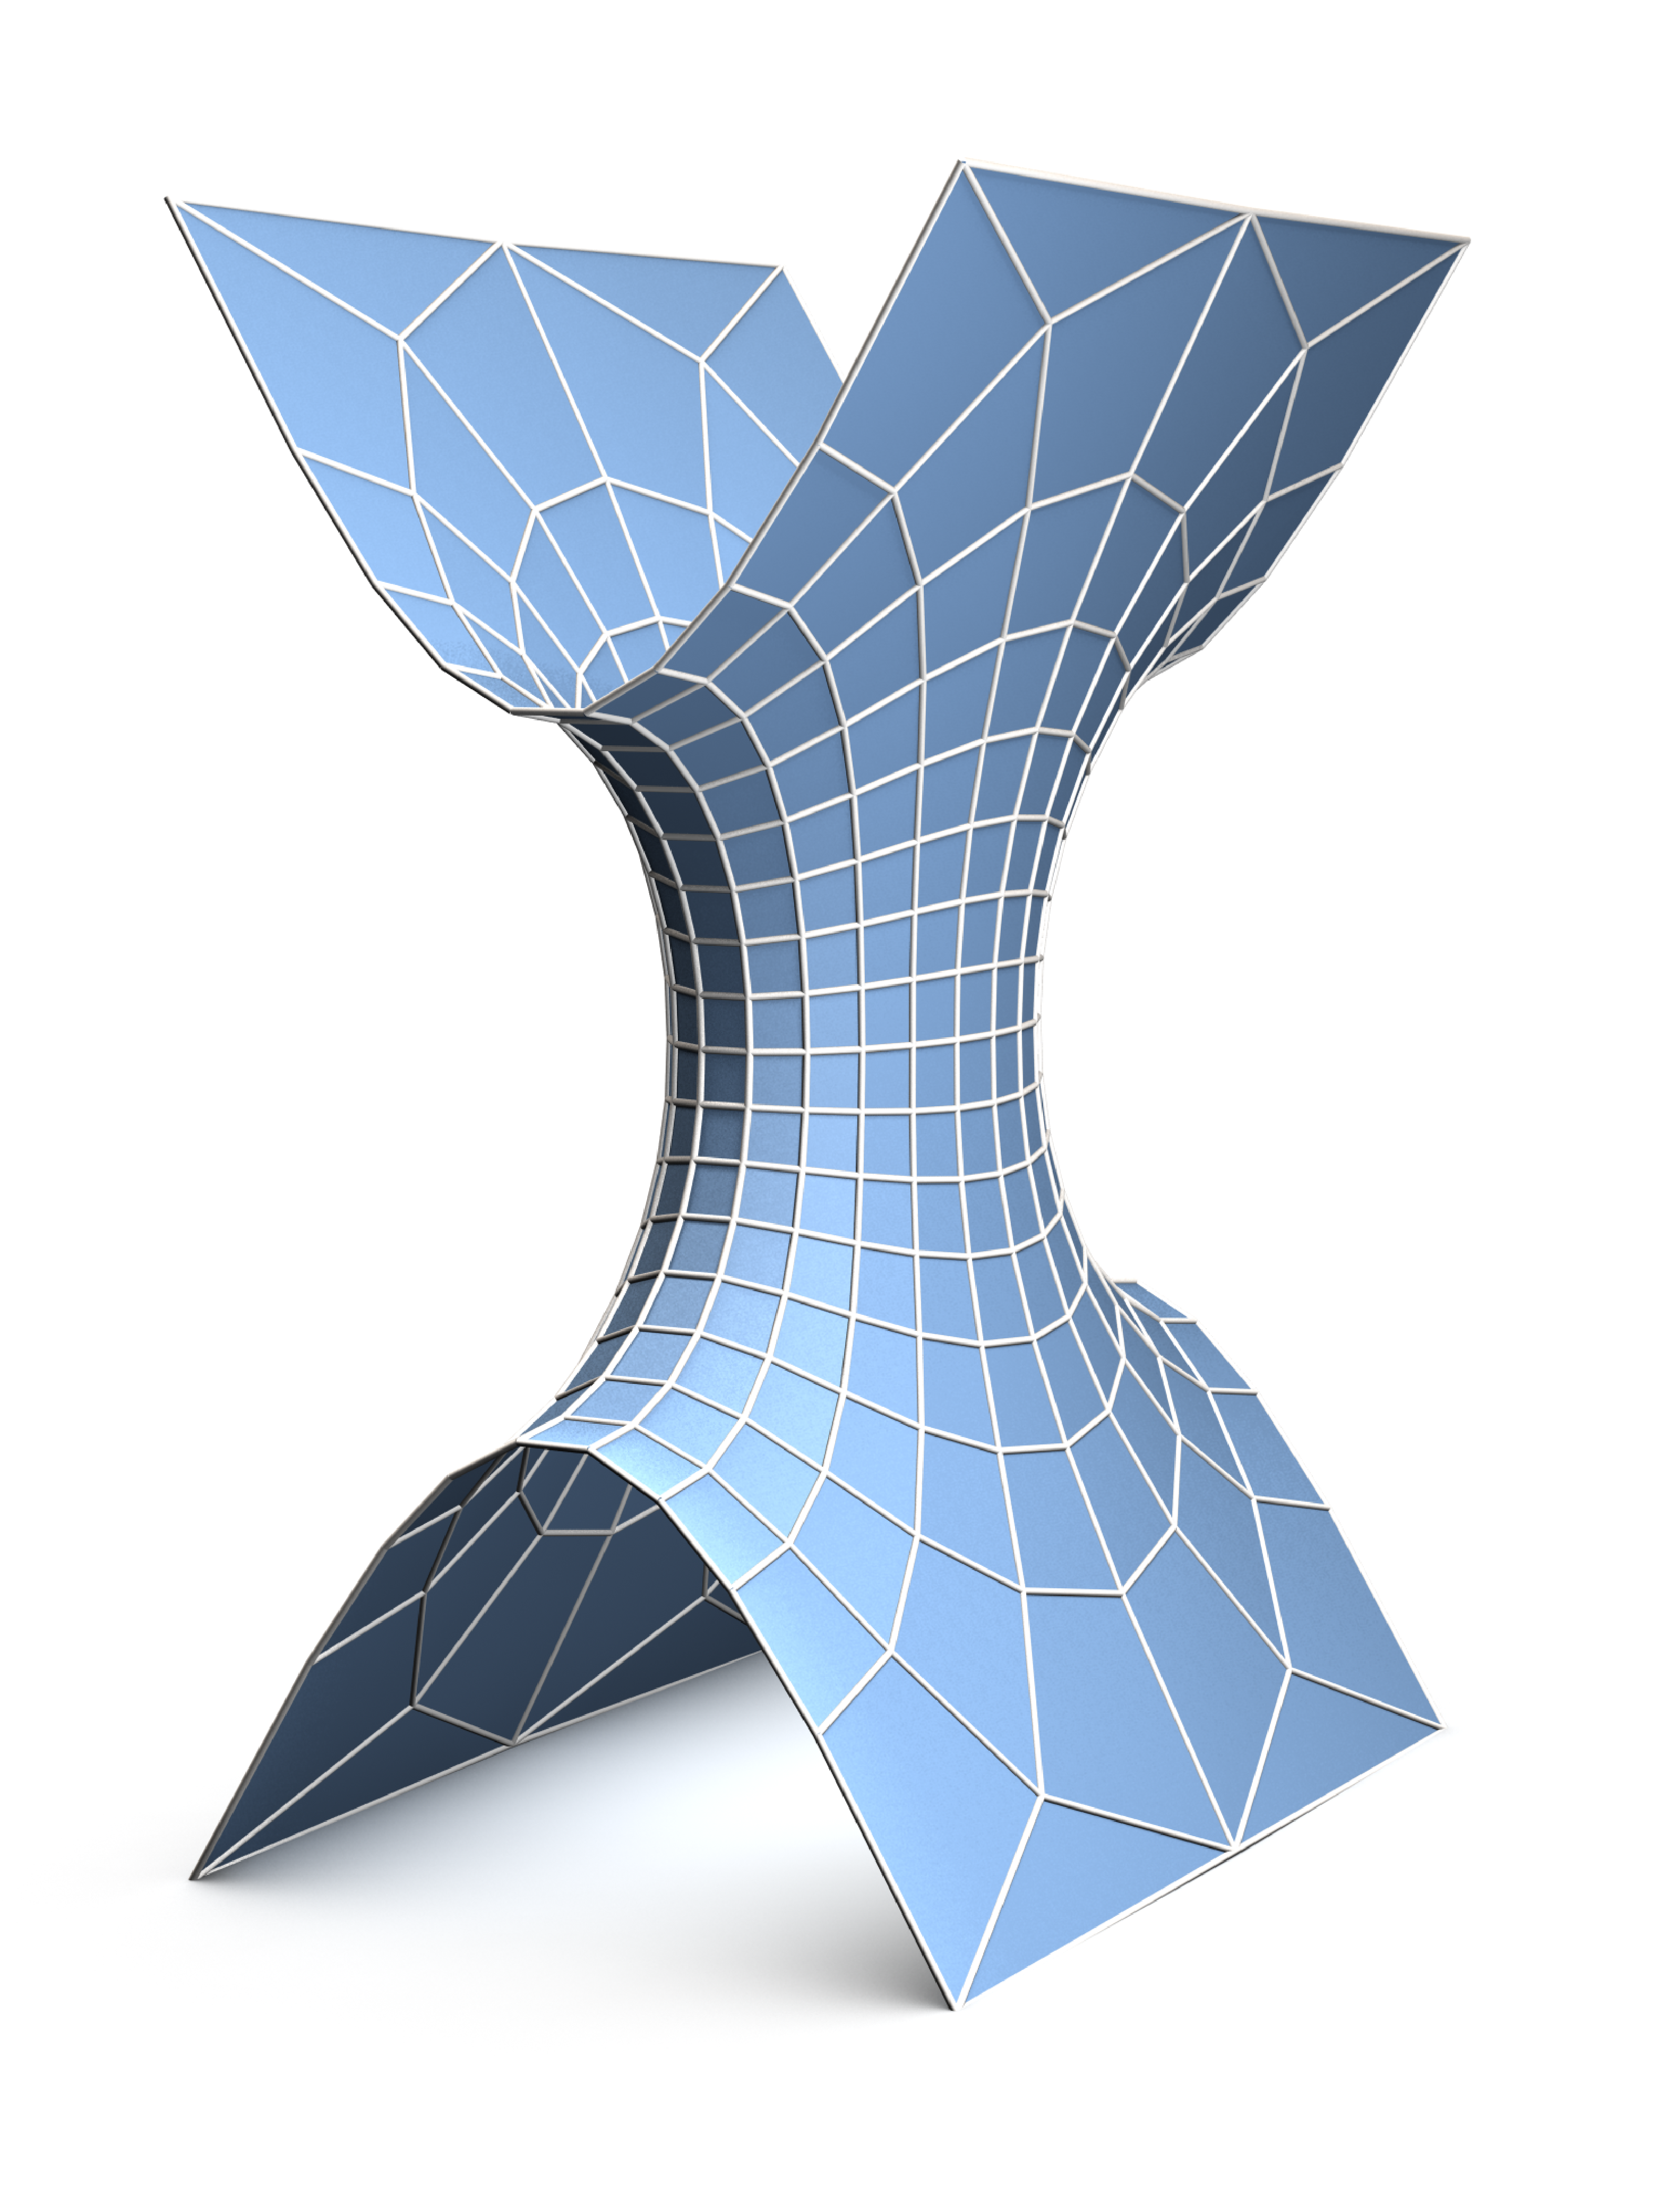
\includegraphics[height=10cm]{image/ellipsoid01_dual.pdf}
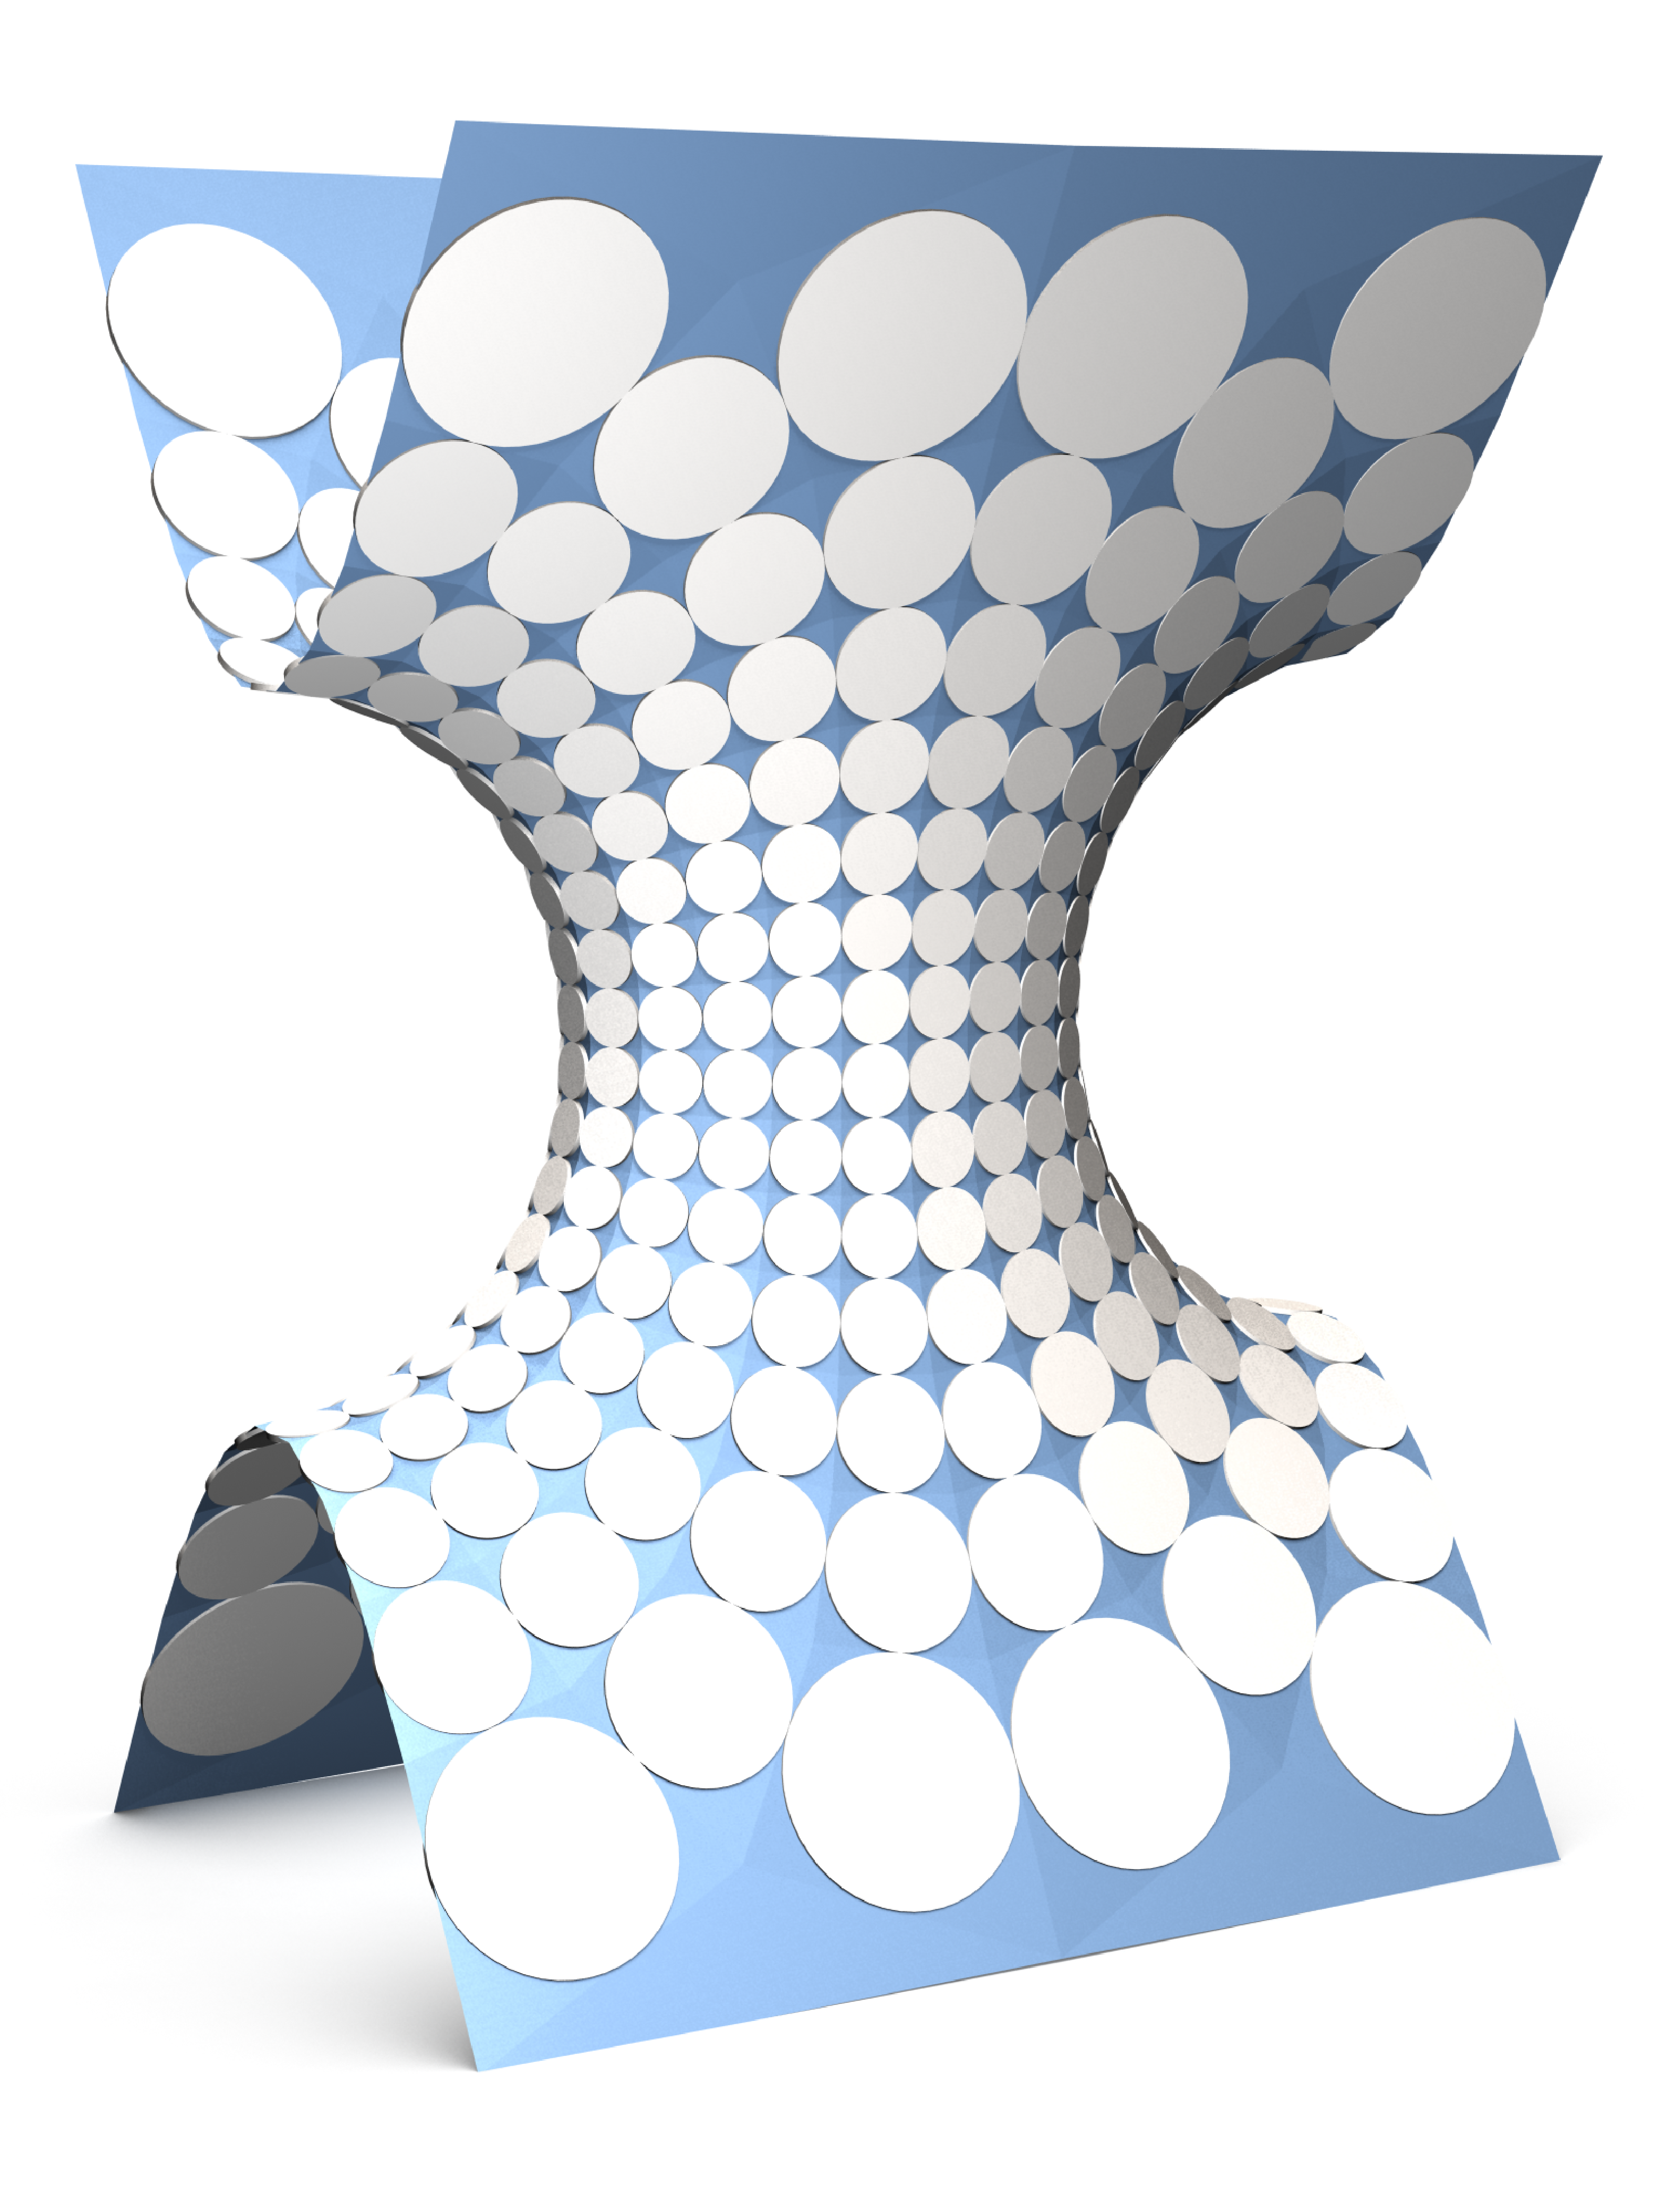
\includegraphics[height=10cm]{image/ellipsoid01_dual_disks.pdf}
}
\caption{Dual surface of discrete s-isothermic ellipsoid of Figure~\ref{fig:ellipsoid}. }
\label{fig:ellipsoid_dual} 
\end{figure}

Here we describe the construction of a discrete s-isothermic ellipsoid and 
its dual surface. (See Hertrich-Jeromin~\cite[p.~202]{Hertrich2003} for the smooth analog).
The rough construction outline is as follows. We start with a discretized version
of the smooth isothermically parameterized ellipsoid. We obtain this by calculating a 
quasiisothermic parameterization of half of a triangulated ellipsoid. After remeshing, 
the parameter lines are approximate curvature lines. We complete the surface by reflection
at the boundary. 
Optimization of the s-isothermic functional yields the final discrete ellipsoid. Its 
dual surface is constructed as in Section~\ref{sub:isometric}.

The connectivity at singularities of the discrete ellipsoid is not unique. If there is a discrete 
curvature line in the symmetry plane of the ellipsoid, we have degenerate quads that have 
vertices with angle $\approx\pi$. The singularity is located at this valence $2$ vertex. 
If there is no discrete curvature line at the symmetry plane then the singularity is located at the 
mid point of the edge connecting two valence three vertices. We have observed that 
the convergence behavior of the s-isothermic functional is considerable better in the former 
model of singularities. We therefore like to call only the discrete ellipsoid with curvature 
lines at symmetry planes a discrete ellipsoid, see Figure~\ref{fig:ellipsoid} and~\ref{fig:ellipsoid_dual}.



\section{Conclusions and future research}
\label{sec:future}
The main contributions of this article are, on the one hand, the definition of 
quasiisothermic parameterizations together with a new algorithm to
compute parameterizations of surfaces that optimizes the corresponding quality measure.
On the other hand, we have defined a new energy for meshes with touching incircles.

We see the main advantage of the algorithm presented in
Section~\ref{sec:parametrization} in its simplicity and its applicability to
shell-like roof structures which arise in architectural models. Since these
models often have almost constant mean curvature and thus allow for an almost
isothermic parameterization, our algorithm performs particularly well on these
examples.

The new energy described in Section~\ref{sec:s-isothermic} is closely related
to the work of Schiftner~\emph{et~al.}~\cite{SchiftnerHWP2009} dealing with
circle packing meshes. They explicitly do not treat quadrilateral meshes since
they are aware of the shape restrictions and focus on triangle meshes instead.
The shape restriction lies in the core of isothermic surfaces but
did not influence our results dramatically for the surfaces in our focus. How
to approximate arbitrary surfaces by isothermic surfaces is unknown and will be
subject to future research. The results of Section~\ref{sec:s-isothermic}
suggest that this might be possible using related methods.

Our new functional generates quad circle packing meshes in the sense of
Schiftner and co-authors. For surfaces arising in architectural context (in
particular for shell-like roofs) we are able to construct aesthetically
pleasing quad meshes supporting a circle packing. 

\subfilebibliography
\end{document}

%%% Local Variables:
%%% TeX-master: "Thesis.tex"
%%% End:

%%!TEX root = ./Thesis.tex
\section[Projective interpolation for arbitrary parameterizations] % for the table of contents
{Projective interpolation for arbitrary parameterizations % normal title
\sectionmark{Projective interpolation} % title on the first page header of section
}
\sectionmark{Projective interpolation} % on other page headers of the sectioin

Let $M=(V, E, F)$ be a triangulated surface consisting of vertices $i\in V$, edges $\it{ij}\in E$ and faces
$\it{ijk}\in F$.



\subsection{Approximation by conformal deformation}
\subsection{Examples}

%%% Local Variables:
%%% TeX-master: "Thesis.tex"
%%% End:
%%!TEX root = ./Thesis.tex

\section{A variational principle for discrete Tschebyshev nets}

Introduction...

\subsection{Variational principle}

Let $M=(V,E,F)$ be a quad-mesh. The vertices of $M$ are denoted by $v_i \in V$, the edges
are $e_{\mathrm{\it{ij}}} \in E$, and the quadrilaterals are denoted by $f_{\mathrm{\it{ijkm}}} \in F$.
\subsection{Energies}
We use a linear combination of energies to enforce desired properties on the optimised mesh.
Our energy consists of three parts.
\begin{equation}
	E(M) =	\lambda_1 E_{\textrm{\scriptsize{ref}}} + 
		\lambda_2 E_{\textrm{\scriptsize{len}}} +
		\lambda_3 E_{\textrm{\scriptsize{cur}}}
	\label{eq:energy_combination}
\end{equation}
The energy $E_{\textrm{\scriptsize{ref}}}$ penalises the distance of vertices from a
reference surface. This surface can be anything that gives a distance function, e.g., a
triangulated surface or a \textsc{Nurbs}-surface. The energy and its gradient are given 
by
\begin{eqnarray*}
	E_{\textrm{\scriptsize{ref}}}(M) &=& 
	\sum_{v_i \in V}\left<v_i - cp_i, v_i - cp_i\right> \\
	\frac{\partial E_\textrm{\scriptsize{ref}}}{\partial v_i} &=&
	2\left(v_i - cp_i\right)
	\label{eq:energy_reference}
\end{eqnarray*}
Here $v_i$ is a vertex of the optimised quad-mesh and $cp_i$ a closest point on the reference
surface measured from vertex $v_i$. The functional $E_{\textrm{\scriptsize{len}}}$ measures
edge length deviation from a given reference length $L$. Its derivative and energy is given as
\begin{eqnarray*}
	E_{\textrm{\scriptsize{len}}}(M) &=& 
	\sum_{e_{\mathrm{\it{ij}}} \in E} \left(\Vert v_i - v_j \Vert - L\right)^2\\
	\frac{\partial E_\textrm{\scriptsize{len}}}{\partial v_i} &=& 
	\sum_{e_{\mathrm{\it{ij}}} \in \textrm{\scriptsize{star}}(v_i)}
	\left(2 - \frac{2L}{\Vert v_i - v_k \Vert}\right)\left(v_i - v_k \right)
\end{eqnarray*}
The sum in the derivative is taken over all edges incident to vertex $v_i$, called the 
edge-star of vertex $v_i$. The third energy is a fairing term that penalises a notion of
curvature of curves on the surface. As we only deal with quad-meshes with $\mathbb Z^2$ combinatorics every interor vertex has four adjacent edges. The energy $E_{\textrm{\scriptsize{cur}}}$ and its gradient is defined as:
\begin{eqnarray*}
	E_{\textrm{\scriptsize{cur}}}(M) &=& \sum_{v_i\in V} \left(\pi - \angle(e_{\mathrm{\it{i1}}}, e_{\mathrm{\it{i3}}}) \right)^2 
	+ \left(\pi - \angle(e_{\mathrm{\it{i2}}}, e_{\mathrm{\it{i4}}}) \right)^2 \\
	\frac{\partial}{\partial v_j}\angle(e_{\mathrm{\it{ij}}},e_{\mathrm{\it{ik}}}) &=& 
	\frac{-1}{\left\Vert e_{\mathrm{\it{ij}}}\right\Vert}\left(e_{\mathrm{\it{ik}}}-e_{\mathrm{\it{ij}}}\frac{\left<e_{\mathrm{\it{ik}}},e_{\mathrm{\it{ij}}}\right>}{\left<e_{\mathrm{\it{ij}}},e_{\mathrm{\it{ij}}}\right>}\right)
	\left\Vert e_{\mathrm{\it{ik}}}-e_{\mathrm{\it{ij}}}\frac{\left<e_{\mathrm{\it{ik}}},e_{\mathrm{\it{ij}}}\right>}		
	{\left<e_{\mathrm{\it{ij}}},e_{\mathrm{\it{ij}}}\right>} \right\Vert^{-1} \\
	\frac{\partial}{\partial v_i}\angle(e_{\mathrm{\it{ij}}},e_{\mathrm{\it{ik}}}) &=& 
	- \left(\frac{\partial}{\partial v_j}\angle(e_{\mathrm{\it{ij}}},e_{\mathrm{\it{ik}}}) + 
	\frac{\partial}{\partial v_k}\angle(e_{\mathrm{\it{ij}}},e_{\mathrm{\it{ik}}})\right)
\end{eqnarray*}
Here and $e_{\mathrm{\it{i1}}}$, $e_{\mathrm{\it{i2}}}$, $e_{\mathrm{\it{i3}}}$, and $e_{\mathrm{\it{i4}}}$ are the adjacent edges of $v_i$ in cyclic order. An edge $e_{\mathrm{\it{ij}}}$ is also used in the role of a vector pointing from vertex $v_i$ to vertex $v_j$. $\angle(e_{\mathrm{\it{ij}}},e_{\mathrm{\it{ik}}})$ is the angle spaned by the vectors $e_{\mathrm{\it{ij}}}$ and $e_{\mathrm{\it{ik}}}$  From the angle derivatives with respect to the vertices the gradient can be computed efficiently.

\begin{figure}[ht]
\centering
\resizebox{\textwidth}{!}{
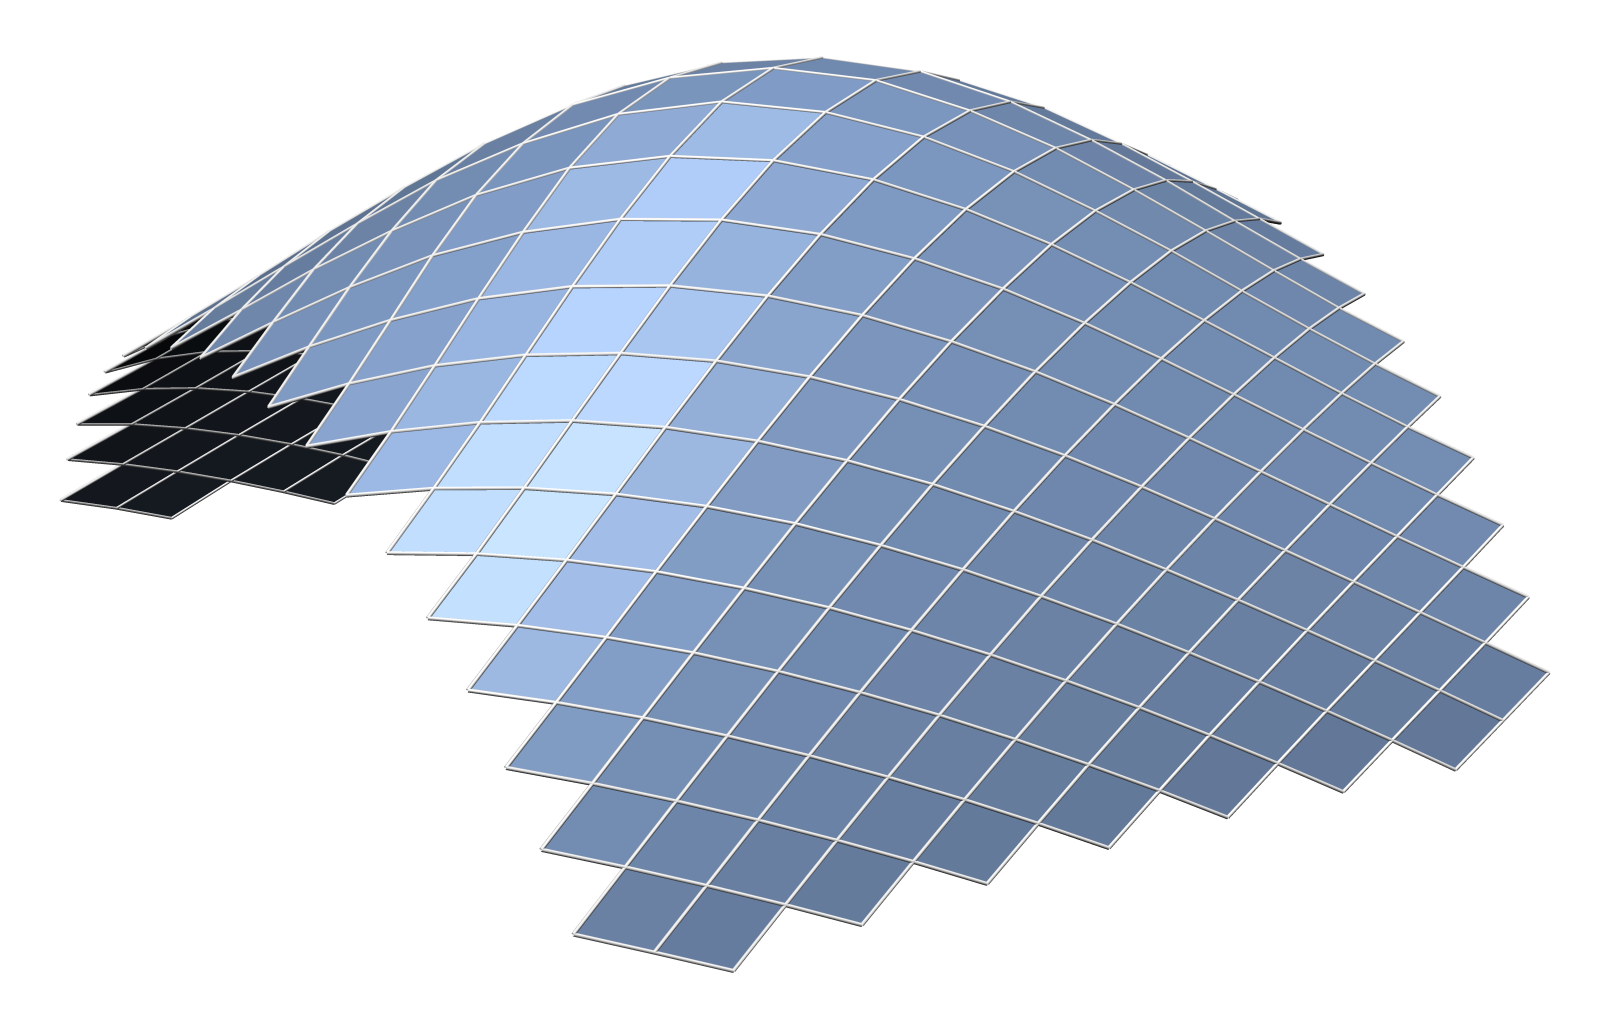
\includegraphics[width=0.33\linewidth]{image/tscheby/init60_mesh.png}
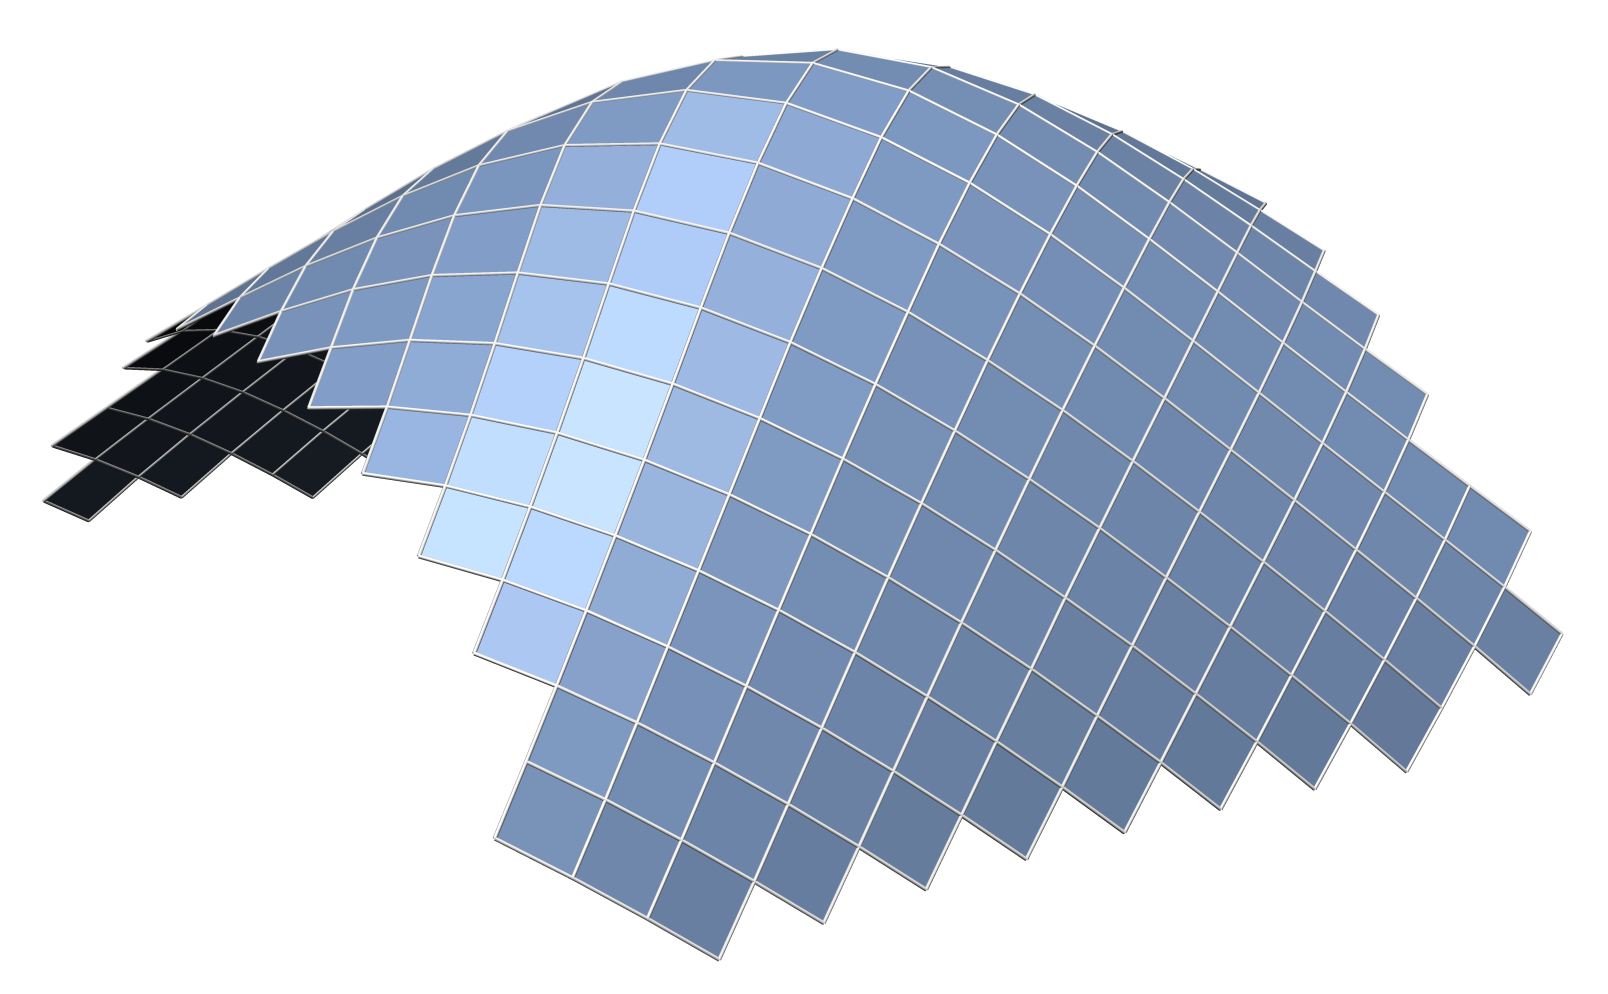
\includegraphics[width=0.33\linewidth]{image/tscheby/init90_mesh.png}
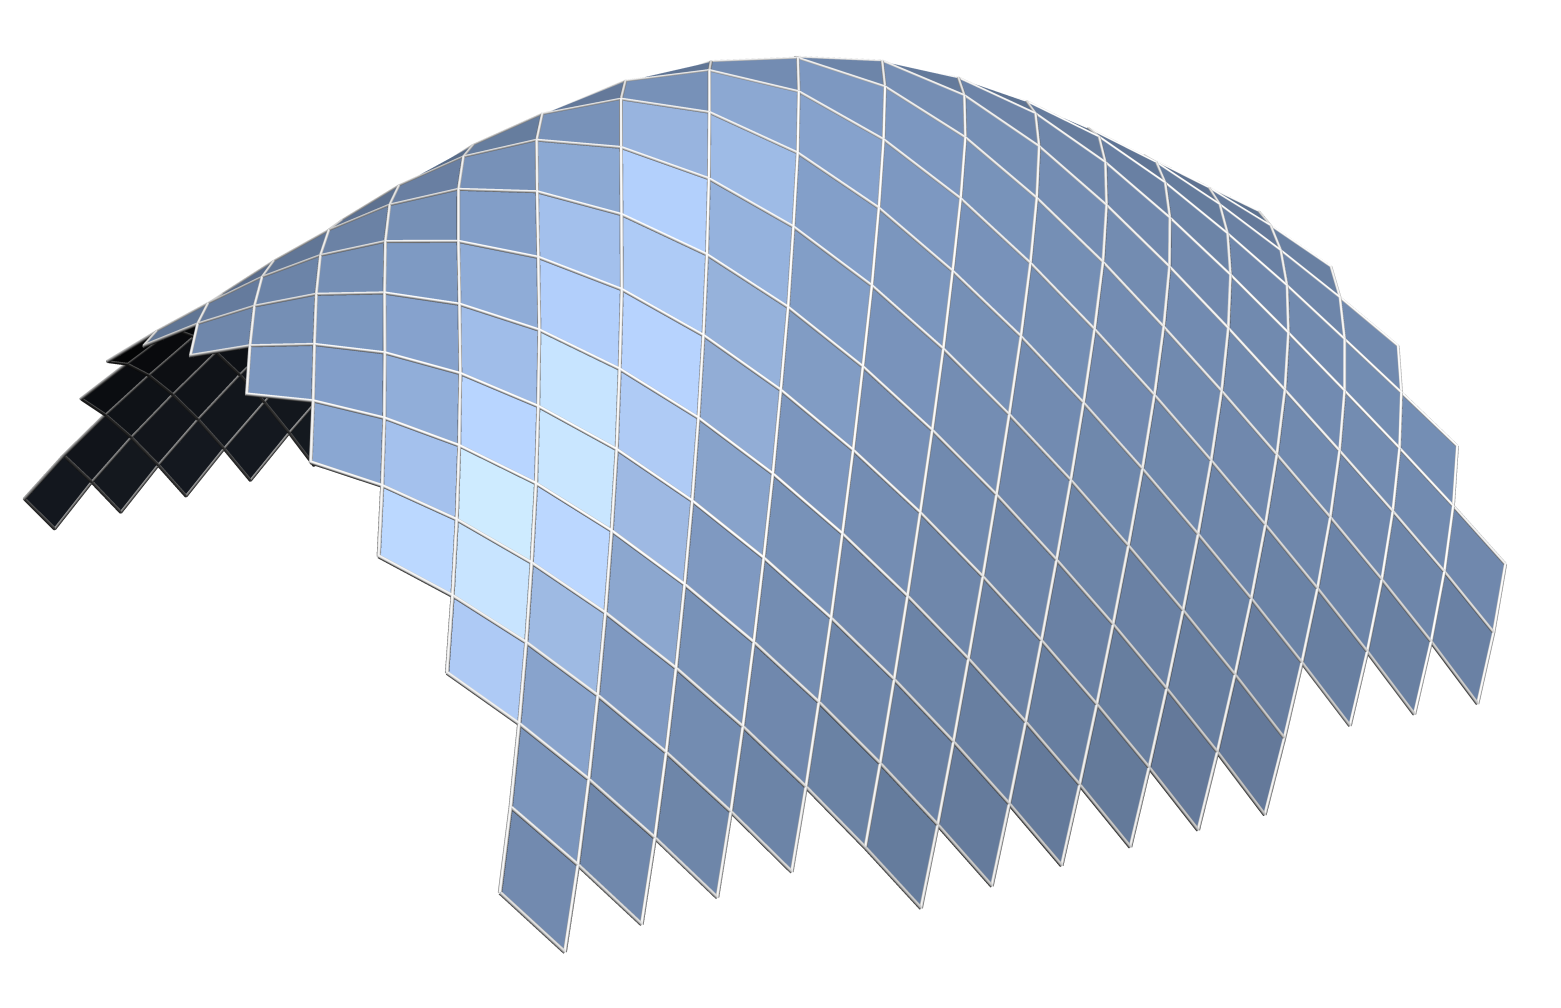
\includegraphics[width=0.33\linewidth]{image/tscheby/init120_mesh.png}
}
\caption{Different initialization shear angles for a conformal remesh. $30^\circ$ left, $0^\circ$ middle, and $-30^\circ$ right.}
\label{fig:initial_grids}
\end{figure}
\subsection{Initialization and parameters}
The energy $E(M)$ is in general non-convex. That means there can be many local optima, and the solution found by some gradient descent depends on the initialisation. We propose to use a conformal remesh of the reference surface as initialization. The conformality of the parameterisation gives us control over the angles between edges of the quadrilaterals. We can introduce shear to the parameterisation and modify this angle globally. By this we start with meshes that have almost constant edge angle (see Fig.~\ref{fig:initial_grids}).

\subsection{Implementation}
We use the conformal mapping algorithm by \cite{Springborn2008} to create the
initial mesh. To minimize the energy $E(M)$ we use the non-linear optimization package
PETSc/TAO \cite{petsc-web-page,tao-user-ref} and its java binding 
\cite{jpetsctao-web-page}. We have made good experiences with normalising the
 energies to have gradient length one before optimization. Then we start with all
$\lambda$s equal to one and modify them on the way if needed. If one encounters
degenerate configurations during optimization one can drop the length energy term for 
a few iterations.

%%% Local Variables:
%%% TeX-master: "Thesis.tex"
%%% End:
%!TEX root = ./Thesis.tex
\chapter{Discrete Differential Geometry - Software Packages}

In the field of Discrete Differential Geometry (DDG) there is a special need for experiments
conducted with the help of computer software. Especially if the methods of DDG are applied
to problems in computer graphics, geometry processing, or architecture, algorithms have 
to be implemented and convincing examples have to be presented. Additionally a suitable 
visualization of the results has to be included in a state-of-the-art publication.

There is a growing knowledge of software development in the mathematical community. This 
is partly due to the curricula of universities which started to include programming courses for undergraduate students.
This enables the students to extend their abilities of creating visualizations and mathematical software, where former generations of students solely used Mathematica and MatLab.

This Chapter is the description and getting-started manual of a set of software packages
(DDG Framework) written in Java. They are specifically designed for the creation of custom interactive software
for experiments with algorithms and geometries treated within DDG. 
Section~\ref{sec:jrworkspace} introduces the {\sc JRWorkspace} library of the {\sc Jtem} project~\cite{JtemWebsite}.
It is the foundation of any application created with the DDG Framework. It is also the user interface basis of {\sc Jreality}, a mathematical visualization library that uses {\sc JRWorkspace} as plug-in and user interface tool~\cite{JrealityWebsite}. In Section~\ref{sec:conformallab} we describe the software {\sc ConformalLab}. This package
implements the methods of the publications~\cite{Bobenko2010, OWR2012, Sechelmann2012, BobSechSpr}.
Section~\ref{sec:varylab} introduces {\sc VaryLab} the software implementation of the methods described in the publications \cite{Lafuente2011, Lafuente2012, Sechelmann2012}.
This package is also released to partners of the development group as {\sc VaryLab[Gridshells]}, {\sc VaryLab[Ultimate]}, or even online as {\sc VaryLab[Service]}.

\begin{figure}
	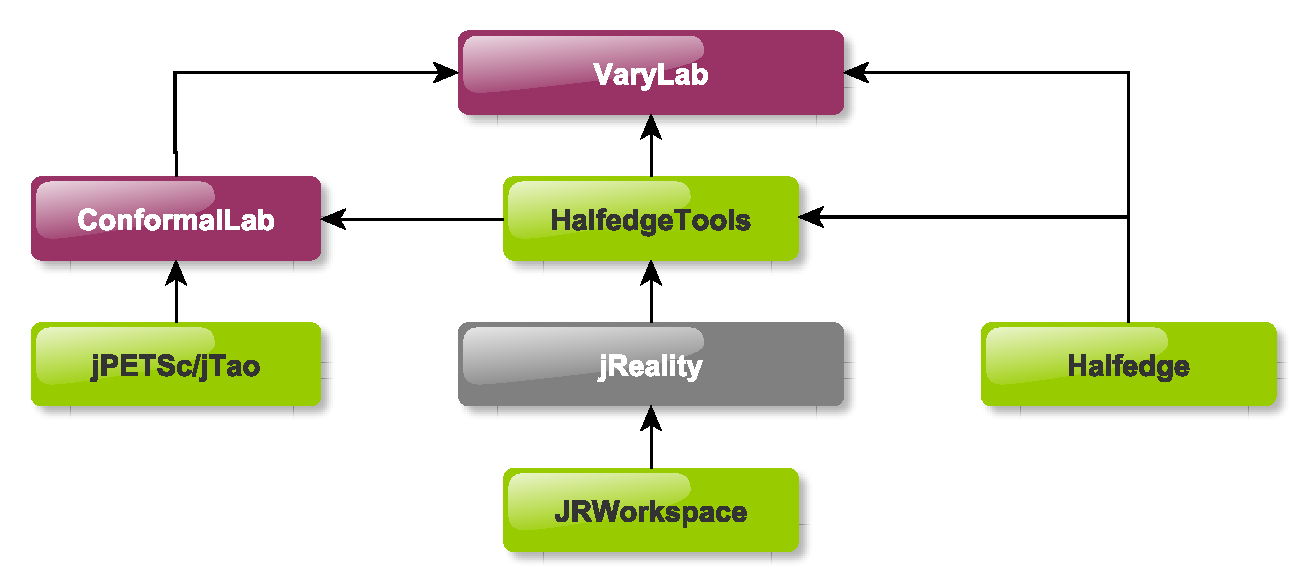
\includegraphics[width=\linewidth]{figures/software_architecture}
	\caption{Software architecture of the DDG Framework}
	\label{fig:software_architecture}
\end{figure}

\section{{\sc JRWorkspace} - A plug-in driven GUI library}

\label{sec:jrworkspace}
\subsection{Plug-ins}
\subsection{Gui elements}
\subsection{{\sc JRWorkspace} and {\sc Jreality}}
\subsection{Building a \emph{jrworkspace} application}

\section{The {\sc Jtem} libraries {\sc Halfedge} and {\sc HalfedgeTools}}
\subsection{The halfedge data structure and tools}
\subsection{Data model and algorithms}

\section{{\sc ConformalLab} - Conformal maps and uniformization}
\label{sec:conformallab}
\subsection{Embedded surfaces}
\subsection{Elliptic and hyperelliptic surfaces}
\subsection{Schottky data}
\subsection{Surfaces with boundary}

\section{{\sc VaryLab} - Variational methods for discrete surfaces}
\label{sec:varylab}
\subsection{Functional plug-ins}
\subsection{Implemented functionals and options}
\subsection{Remeshing}

\section{U3D - 3D content in presentations and online publiciations}
\label{sec:u3d}
\subsection{3D content in PDF documents}

\section{Non-linear optimization with jPETSc/jTao}
\label{sec:jpetsctao}
\subsection{A java wrapper for PETSc/Tao}

%%% Local Variables:
%%% TeX-master: "Thesis.tex"
%%% End:

\newpage
\backmatter 
\bibliographystyle{alpha}
%disable numbering 
\setcounter{secnumdepth}{-1} 
\bibliography{Thesis}

\chapter{Acknowledgements}


\end{document}